\documentclass[aspectratio=169,]{beamer}

% -------------------------------------------------------------------------
% 1. REQUIRED PACKAGES (The "Batteries" Quarto usually includes)
% -------------------------------------------------------------------------
\usepackage{graphicx}
\usepackage{booktabs}
\usepackage{longtable}
\usepackage{hyperref}
\usepackage{array}      % <--- ADD THIS LINE HERE
\usepackage[most]{tcolorbox} % REQUIRED for Quarto Callouts
\usepackage{fontawesome5}    % REQUIRED for Callout Icons
\usepackage{framed}          % REQUIRED for standard blocks
\usepackage{tikz}
\usetikzlibrary{arrows.meta}

% Fix for Pandoc's "tightlist"
\providecommand{\tightlist}{%
  \setlength{\itemsep}{0pt}\setlength{\parskip}{0pt}}

% -------------------------------------------------------------------------
% 2. CUSTOM DESIGN PACKAGES
% -------------------------------------------------------------------------
\usepackage{tikz}
\usepackage{calc}
\usepackage{xcolor}
\usepackage{xparse} 
\usepackage{etoolbox} 
\usepackage[default]{sourcesanspro} 
\usetikzlibrary{calc, positioning, shapes.geometric}

% -------------------------------------------------------------------------
% DEFINE QUARTO CALLOUT COLORS (REQUIRED)
% -------------------------------------------------------------------------
% We map these to your "Elegant Dark Mode" aesthetic.
% Note: Quarto expects these EXACT names.

% 1. Note (Blue)
\definecolor{quarto-callout-note-color}{HTML}{3498DB}        % Icon/Title Color
\definecolor{quarto-callout-note-color-frame}{HTML}{2980B9}  % Border Color

% 2. Tip (Green)
\definecolor{quarto-callout-tip-color}{HTML}{27AE60}
\definecolor{quarto-callout-tip-color-frame}{HTML}{2ECC71}

% 3. Important (Red/Crimson)
\definecolor{quarto-callout-important-color}{HTML}{C0392B}
\definecolor{quarto-callout-important-color-frame}{HTML}{E74C3C}

% 4. Warning (Orange)
\definecolor{quarto-callout-warning-color}{HTML}{F39C12}
\definecolor{quarto-callout-warning-color-frame}{HTML}{E67E22}

% 5. Caution (Yellow/Gold)
\definecolor{quarto-callout-caution-color}{HTML}{F1C40F}
\definecolor{quarto-callout-caution-color-frame}{HTML}{D4AC0D}

% Add this right before \begin{document}
\newcommand{\Est}[1]{\textcolor{quarto-callout-important-color}{\mathbf{#1}}}

\providecommand{\estc}[1]{\textcolor[HTML]{1B7837}{#1}}
\makeatletter
\@ifpackageloaded{caption}{}{\usepackage{caption}}
\AtBeginDocument{%
\ifdefined\contentsname
  \renewcommand*\contentsname{Table of contents}
\else
  \newcommand\contentsname{Table of contents}
\fi
\ifdefined\listfigurename
  \renewcommand*\listfigurename{List of Figures}
\else
  \newcommand\listfigurename{List of Figures}
\fi
\ifdefined\listtablename
  \renewcommand*\listtablename{List of Tables}
\else
  \newcommand\listtablename{List of Tables}
\fi
\ifdefined\figurename
  \renewcommand*\figurename{Figure}
\else
  \newcommand\figurename{Figure}
\fi
\ifdefined\tablename
  \renewcommand*\tablename{Table}
\else
  \newcommand\tablename{Table}
\fi
}
\@ifpackageloaded{float}{}{\usepackage{float}}
\floatstyle{ruled}
\@ifundefined{c@chapter}{\newfloat{codelisting}{h}{lop}}{\newfloat{codelisting}{h}{lop}[chapter]}
\floatname{codelisting}{Listing}
\newcommand*\listoflistings{\listof{codelisting}{List of Listings}}
\makeatother
\makeatletter
\makeatother
\makeatletter
\@ifpackageloaded{caption}{}{\usepackage{caption}}
\@ifpackageloaded{subcaption}{}{\usepackage{subcaption}}
\makeatother

% -------------------------------------------------------------------------
% NEW: COLOR THEME COMMANDS (Robust Single-Slide Overrides)
% -------------------------------------------------------------------------

% 1. Light Mode Command
\newcommand{\LightMode}{
  % 1. Draw White Background (TikZ Overlay)
  \begin{tikzpicture}[remember picture, overlay]
    \fill[white] (current page.south west) rectangle (current page.north east);
  \end{tikzpicture}
  % 2. Force Text Colors to Black
  \setbeamercolor{normal text}{fg=black}
  \setbeamercolor{frametitle}{fg=black}
  \setbeamercolor{itemize item}{fg=black}
  \setbeamercolor{structure}{fg=black}
  \usebeamercolor[fg]{normal text}
}

% 2. Black Mode Command
\newcommand{\BlackMode}{
  \begin{tikzpicture}[remember picture, overlay]
    \fill[black] (current page.south west) rectangle (current page.north east);
  \end{tikzpicture}
  \setbeamercolor{normal text}{fg=white}
  \setbeamercolor{frametitle}{fg=white}
  \setbeamercolor{itemize item}{fg=white}
  \setbeamercolor{structure}{fg=white}
  \usebeamercolor[fg]{normal text}
}

% 3. Brand Mode Command
\newcommand{\BrandMode}{
  \begin{tikzpicture}[remember picture, overlay]
    \definecolor{tempBrand}{HTML}{7D181E}
    \fill[tempBrand] (current page.south west) rectangle (current page.north east);
  \end{tikzpicture}
  \setbeamercolor{normal text}{fg=white}
  \setbeamercolor{frametitle}{fg=white}
  \setbeamercolor{itemize item}{fg=white}
  \setbeamercolor{structure}{fg=white}
  \usebeamercolor[fg]{normal text}
}

% -------------------------------------------------------------------------
% 4. UC BERKELEY THEME (Modern Matte) - FIXED SCOPE
% -------------------------------------------------------------------------

% 1. DEFINE COLORS GLOBALLY (Required for assumptionbox and modes)
\definecolor{BerkeleyBlue}{HTML}{003262}
\definecolor{CaliforniaGold}{HTML}{FDB515}
\definecolor{BerkeleyMatte}{HTML}{0D2D52} 
\definecolor{SoftWhite}{HTML}{F8F9FA}

% 4. UC Berkeley Theme (Modern Matte)
\newcommand{\BerkeleyMode}{
  % 2. Draw Background AND Title
  \begin{tikzpicture}[remember picture, overlay]
    % Background Fill (Covers old title)
    \fill[BerkeleyMatte] (current page.south west) rectangle (current page.north east);
    % Gold Accent Strip
    \fill[CaliforniaGold] (current page.south west) rectangle ($(current page.north west)+(0.15cm,0)$);
    % REDRAW TITLE ON TOP
    \node[anchor=west, white, font=\Large\bfseries] at ($(current page.north west)+(1cm,-1cm)$) {\insertframetitle};
  \end{tikzpicture}
  
  % 3. Set Text Colors
  \setbeamercolor{normal text}{fg=SoftWhite}
  \setbeamercolor{frametitle}{fg=BerkeleyMatte} % Hide original title
  \setbeamercolor{itemize item}{fg=CaliforniaGold} 
  \setbeamercolor{structure}{fg=CaliforniaGold}
  
  \usebeamercolor[fg]{normal text}
}

% 5. UC Berkeley Theme (Academic Light)
\newcommand{\BerkeleyLightMode}{
  % (Color definitions removed here as they are now global)
  
  % 2. Draw Background AND Title
  \begin{tikzpicture}[remember picture, overlay]
    % Background Fill
    \fill[white] (current page.south west) rectangle (current page.north east);
    % Blue Header Bar
    \fill[BerkeleyBlue] (current page.north west) rectangle ($(current page.north east)+(0,-1.4cm)$);
    % Gold Line
    \fill[CaliforniaGold] ($(current page.north west)+(0,-1.4cm)$) rectangle ($(current page.north east)+(0,-1.45cm)$);
    % REDRAW TITLE ON TOP
    \node[anchor=west, white, font=\Large\bfseries] at ($(current page.north west)+(1cm,-0.7cm)$) {\insertframetitle};
  \end{tikzpicture}
  
  % 3. Set Text Colors
  \setbeamercolor{normal text}{fg=black}
  \setbeamercolor{frametitle}{fg=white} 
  \setbeamercolor{itemize item}{fg=BerkeleyBlue}
  \setbeamercolor{structure}{fg=BerkeleyBlue}
  
  \usebeamercolor[fg]{normal text}
}

% -------------------------------------------------------------------------
% NEW: ACADEMIC POWER LAYOUTS
% -------------------------------------------------------------------------

% 1. Statement Layout (Big Impact Transitions)
% Usage: ::: {.layout-statement} Content :::
\newenvironment{layout-statement}{
  \vspace*{\fill}
  \centering
  \Huge \bfseries
  \setbeamercolor{normal text}{fg=CaliforniaGold} % Use Gold for impact
  \usebeamercolor[fg]{normal text}
}{
  \vspace*{\fill}
}

% 2. Dense Data Layout (Regression Tables)
% Usage: ::: {.layout-dense} Table :::
\newenvironment{layout-dense}{
  \vspace*{\fill}
  \tiny                  % Force tiny font
  \setlength\tabcolsep{2pt} % Tighten table columns
  \centering
}{
  \vspace*{\fill}
}

% 3. Split Slide Macro (Vertical Centering)
% Usage: \SplitSlide{Left Content}{Right Content}
\newcommand{\SplitSlide}[2]{
  \begin{columns}[c] % 'c' option forces vertical centering
    \begin{column}{0.48\textwidth}
      #1
    \end{column}
    \begin{column}{0.48\textwidth}
      \centering
      #2
    \end{column}
  \end{columns}
}

% -------------------------------------------------------------------------
% 3. DYNAMIC BACKGROUND & CONTRAST LOGIC
% -------------------------------------------------------------------------
  \definecolor{mainbg}{HTML}{0D2D52}

\setbeamercolor{background canvas}{bg=mainbg}

% Logic to calculate luminance and set text color automatically
\makeatletter
\newcommand{\AutoSetContrast}{
  \extractcolorspec{mainbg}{\mainbgspec}
  \expandafter\convertcolorspec\mainbgspec{rgb}\mainbgrgb
  \def\calculatebrightness##1,##2,##3;{
    \pgfmathparse{0.2126*##1 + 0.7152*##2 + 0.0722*##3}
  }
  \expandafter\calculatebrightness\mainbgrgb;
  \pgfmathparse{\pgfmathresult > 0.5 ? 1 : 0}
  \ifnum\pgfmathresult=1
    \definecolor{maintext}{HTML}{222222}
    \definecolor{dimtext}{HTML}{555555}
  \else
    \definecolor{maintext}{HTML}{FFFFFF}
    \definecolor{dimtext}{HTML}{CCCCCC}
  \fi
}
\makeatother

\AutoSetContrast

\setbeamercolor{normal text}{fg=maintext}
\setbeamercolor{frametitle}{fg=maintext}
\setbeamercolor{title}{fg=maintext}
\setbeamercolor{structure}{fg=maintext} 

% -------------------------------------------------------------------------
% 4. FOOTER CUSTOMIZATION
% -------------------------------------------------------------------------
\setbeamercolor{footline}{fg=dimtext}
\setbeamerfont{footline}{size=\tiny}

\newtoggle{hidesection}
\togglefalse{hidesection}

\setbeamertemplate{footline}{
  \begin{beamercolorbox}[wd=\paperwidth, ht=2.5ex, dp=1.125ex, leftskip=.3cm, rightskip=.3cm]{footline}
    \iftoggle{hidesection}{}{
      \insertsectionhead
    }
    \hfill
    \insertframenumber
  \end{beamercolorbox}
}
\setbeamertemplate{navigation symbols}{}

% -------------------------------------------------------------------------
% 5. CUSTOM COMMANDS & ENVIRONMENTS (FIXED FOR STABILITY)
% -------------------------------------------------------------------------
\NewDocumentCommand{\navbutton}{ O{} O{fill=gray} m }{
  \hyperlink{#1}{
    \tikz[baseline=(node.base)]{
      \node(node)[
        anchor=base,
        rounded corners=3pt,
        inner sep=5pt,
        text=white,
        font=\small\bfseries,
        #2
      ]{#3};
    }
  }
}

\newenvironment{layout-math}{
  \vspace*{\fill}
  \centering
  \begin{minipage}{\linewidth}
  \centering
}{
  \end{minipage}
  \vspace*{\fill}
}

% SAFE Layout for Tables (Removed risky \makebox)
\newenvironment{layout-table}{
  \vspace*{\fill}
  \begin{center}
}{
  \end{center}
  \vspace*{\fill}
}

% SAFE Layout for Full Figures (Uses LRBOX to capture content first)
\newsavebox{\fullfigbox}
\newenvironment{layout-full-figure}{
  \begin{lrbox}{\fullfigbox}
    \begin{minipage}{\paperwidth}
      \centering
}{
    \end{minipage}
  \end{lrbox}
  \begin{tikzpicture}[remember picture, overlay]
    \node[anchor=center, inner sep=0pt] at (current page.center) {
      \usebox{\fullfigbox}
    };
  \end{tikzpicture}
}

\newcommand{\hidefootersection}{\global\toggletrue{hidesection}}
\newcommand{\showfootersection}{\global\togglefalse{hidesection}}


% -------------------------------------------------------------------------
% CUSTOM BERKELEY CALLOUT BOX
% -------------------------------------------------------------------------
\newtcolorbox{assumptionbox}[1]{
  enhanced,
  colback=SoftWhite,       % White-ish background
  colframe=CaliforniaGold, % Gold Border
  coltitle=SoftWhite,      % White Title Text
  colbacktitle=BerkeleyMatte, % Berkeley Blue Title Background
  title={#1},
  fonttitle=\bfseries\small,
  arc=2pt,                 % Slight rounded corners
  boxrule=1pt,             % Thin elegant border
  left=5pt, right=5pt, top=5pt, bottom=5pt, % Padding
  titlerule=0pt,
  width=\linewidth
}

% -------------------------------------------------------------------------
% 6. DOCUMENT BODY
% -------------------------------------------------------------------------
\title{Internalizing Environmental Risk: Insurance Design and Firm
Behavior in Hazardous Industries}
\author{Kaleb K. Javier}

\begin{document}

\frame{\titlepage}

\begin{frame}{Strict liability is the primary instrument for
environmental harm}
\phantomsection\label{strict-liability-is-the-primary-instrument-for-environmental-harm}
\BerkeleyLightMode

\begin{itemize}
\tightlist
\item
  The firm pays for what it causes, regardless of fault --- across oil
  \& gas (OPA 1990), surface mining (SMCRA 1977), and hazardous
  substances (CERCLA 1980, RCRA 1976)
\item
  Works when firms can be held fully accountable --- breaks down when
  they cannot (Shavell 1986, 2007)
\item
  Shavell (2004): two instruments to restore accountability:

  \begin{itemize}
  \tightlist
  \item
    Minimum Asset / bonding requirements
  \item
    \textbf{Compulsory liability insurance} --- where the premium does
    the deterrence work, \emph{if} the insurer can price on
    risk-relevant attributes
  \end{itemize}
\end{itemize}

\vfill

\centering\textbf{This paper examines the design and efficacy of compulsory liability insurance as a financial responsibility instrument in environmental hazard settings.}
\end{frame}

\begin{frame}{Does insurance design change firm behavior?}
\phantomsection\label{does-insurance-design-change-firm-behavior}
\BerkeleyLightMode

\textbf{Setting}

\begin{itemize}
\tightlist
\item
  USTs --- retail petroleum storage, \(\sim\),140,000 facilities, the
  most common source of groundwater contamination in the US (EPA 2024)
\item
  Compulsory insurance the law since 1988 (RCRA Subtitle I, \$1M floor)
\item
  \textbf{Clean shock:} Texas exits its flat-fee fund December 22, 1998
  --- 26,000 facilities enter risk-rated private insurance overnight
\item
  9.8M tank-years of EPA panel data spanning both regimes
\end{itemize}

\vspace{0.2cm}

\textbf{Three questions}

\begin{itemize}
\tightlist
\item
  \textbf{Q1 --- Observability:} Is release risk predictable from
  observable tank characteristics?
\item
  \textbf{Q2 --- Behavior:} Does risk-based pricing change closure,
  replacement, and release outcomes?
\item
  \textbf{Q3 --- Welfare:} How much of the first-best welfare gain does
  risk-rated pricing capture?
\end{itemize}
\end{frame}

\begin{frame}{What is an underground storage tank?}
\phantomsection\label{what-is-an-underground-storage-tank}
\BerkeleyLightMode

{[}ADD FIGURE HERE{]}
\end{frame}

\begin{frame}{Related literature}
\phantomsection\label{related-literature}
\BerkeleyLightMode

\small

\textbf{Liability regimes, financial responsibility, and UST policy}

Shavell (1986, 2004, 2007); Yin, Kunreuther \& White (2011); Yin, Pfaff
\& Kunreuther (2011, 2007); Boomhower (2019); Ho, Hsu, Cha \& Rivera
(2018)

\emph{First firm-level panel analysis of insurance design --- risk-rated
vs.~flat-fee --- as a financial responsibility instrument; clean policy
shock; structural welfare decomposition}

\medskip

\textbf{Environmental economics and environmental risk}

Fowlie, Reguant \& Ryan (2016); Muehlenbachs (2015); Blundell,
Gowrisankaran \& Langer (2020); Kellogg \& Reguant (2021)

\emph{Dynamic structural model of firm behavior under environmental
regulation; welfare decomposition bounding gap to first-best}

\medskip

\textbf{IO of selection markets: risk-based and cost-based pricing}

Einav, Finkelstein \& Mahoney (2021); Einav, Finkelstein \& Cullen
(2010); Bundorf, Levin \& Mahoney (2012); Handel, Hendel \& Whinston
(2015); Mahoney \& Weyl (2017)

\emph{{[}PLACEHOLDER{]}}
\end{frame}

\begin{frame}{}
\phantomsection\label{section}
\BerkeleyMode

\begin{center}
\Huge \textbf{Setting, Data, and Observability}
\end{center}
\end{frame}

\begin{frame}{Who operates USTs?}
\phantomsection\label{who-operates-usts}
\BerkeleyLightMode

\vspace{0.3cm}
\begin{center}
\small
\renewcommand{\arraystretch}{1.25}
\begin{tabular}{lcc}
\hline
\textbf{Operator type} & \textbf{Share of facilities} & \textbf{Share of tanks} \\
\hline
Independent retail (gas station / c-store) & [XX]\% & [XX]\% \\
Branded / major oil company                & [XX]\% & [XX]\% \\
Fleet / non-retail (trucking, municipal)   & [XX]\% & [XX]\% \\
Government / other                         & [XX]\% & [XX]\% \\
\hline
\end{tabular}
\end{center}

\begin{itemize}
\tightlist
\item
  \textbf{{[}xyz type is dominat type in sample{]}} --- retail gas
  stations, truck stops, and fleet facilities account for {[}XX{]}\% of
  operators; branded majors are a minority
\item
  \(\sim\),140,000 active facilities at peak; \(\sim\),550,000 tanks
  nationwide
\item
  Median facility: {[}X{]} active tanks, {[}XXX{]}k gallons total
  capacity
\end{itemize}
\end{frame}

\begin{frame}{Release risk varies with observable tank traits}
\phantomsection\label{release-risk-varies-with-observable-tank-traits}
\BerkeleyLightMode

\begin{itemize}
\tightlist
\item
  Annual release probability is driven by \textbf{tank age} and
  \textbf{wall construction}
\item
  Single-walled steel: no secondary containment, corrodes gradually,
  hazard rises steeply with age
\item
  Double-walled: interstitial monitoring space, hazard flat and low
  across all ages
\item
  Key observables: age, wall type, piping, leak-detection technology ---
  exactly what an underwriter can verify
\end{itemize}

\vfill

\centering\small\textit{Whether the private market prices this heterogeneity is an empirical question --- answered after we set up the data.}
\end{frame}

\begin{frame}{The harm is silent, slow, and diffuse --- tort law cannot
reach it}
\phantomsection\label{the-harm-is-silent-slow-and-diffuse-tort-law-cannot-reach-it}
\BerkeleyLightMode

\begin{itemize}
\tightlist
\item
  No secondary containment, no visible event, no immediate victim
\item
  Benzene and petroleum migrate silently into groundwater; by detection
  the plume may have traveled hundreds of feet
\item
  Diffuse victims, delayed injury, causation hard to establish ---
  private tort law does not operate here
\item
  Health damages \(\sim\),\$17k per release (Marcus 2021) generate no
  insurance claim: contamination unobservable, victims cannot sue
\end{itemize}

\vfill

\centering\small\textit{The regulatory system --- compulsory insurance --- is the only operative instrument.}
\end{frame}

\begin{frame}{Releases are costly to cleanup budgets and human health}
\phantomsection\label{releases-are-costly-to-cleanup-budgets-and-human-health}
\BerkeleyLightMode

\vspace{0.2cm}
\begin{center}
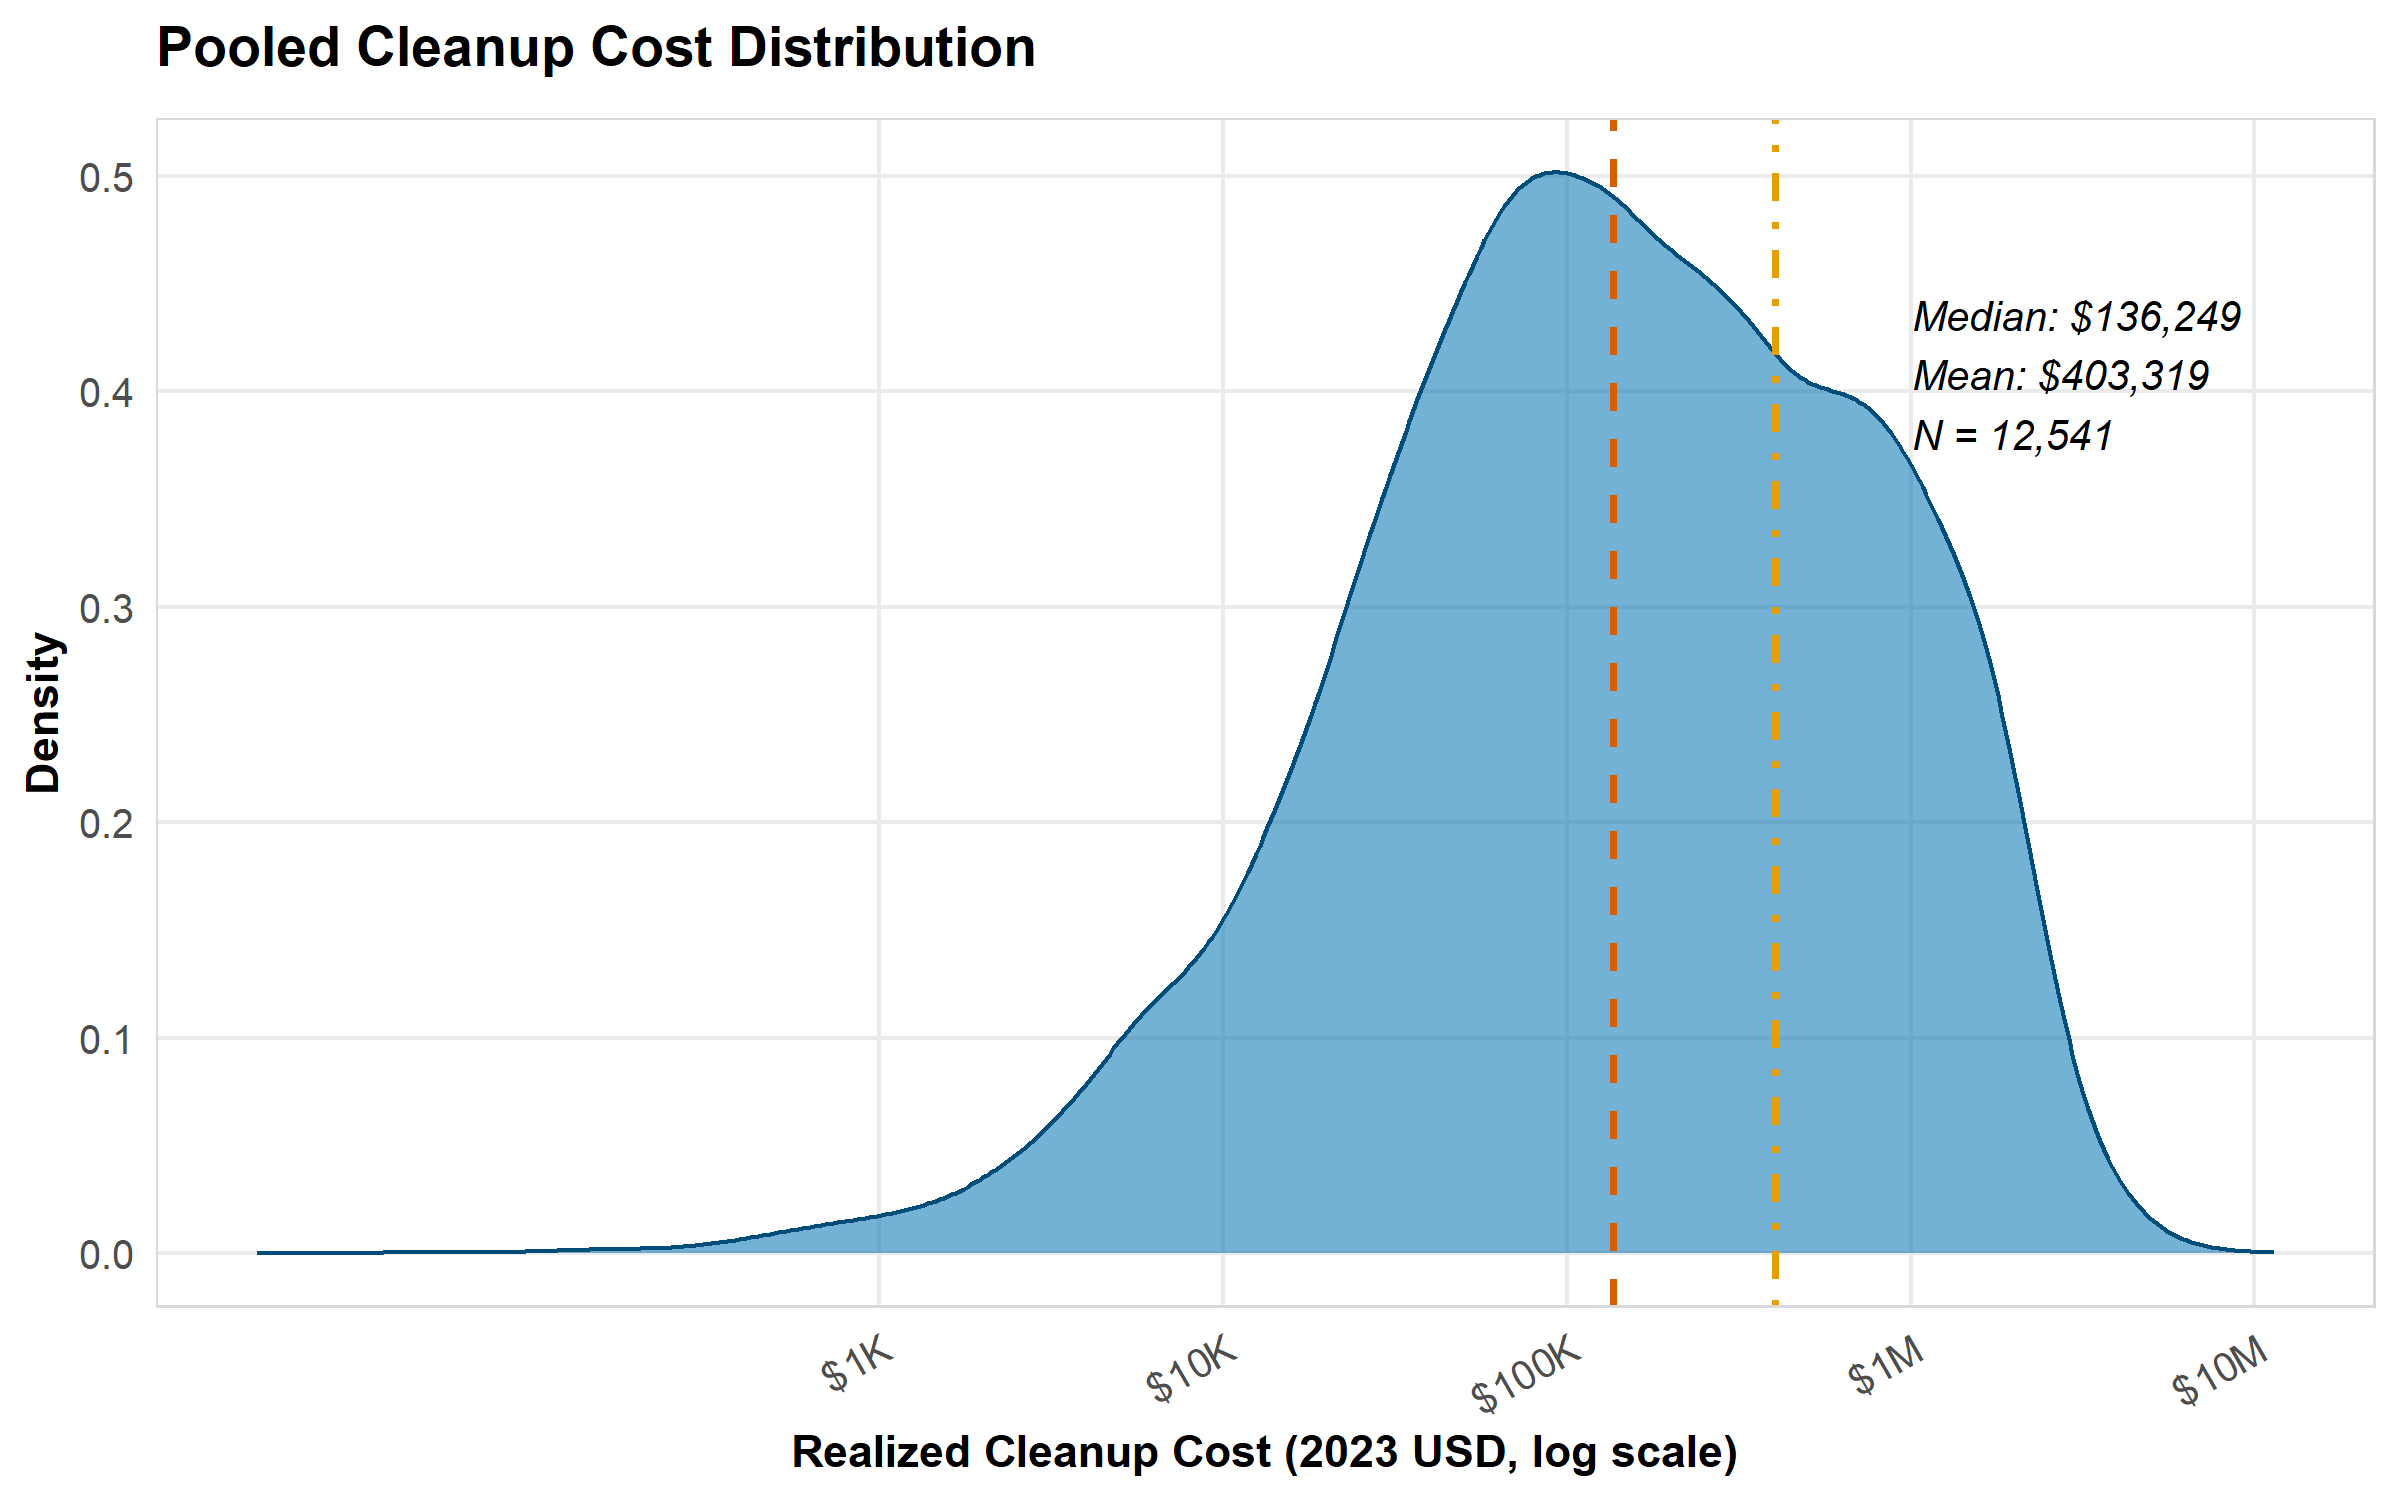
\includegraphics[height=0.72\textheight,keepaspectratio]{../../Output/Figures/Figure_cost_distribution_pooled.png}
\end{center}

\vfill

\centering\small\textit{$\sim$\,550,000 confirmed releases since 1988. Median cleanup \$136k; mean \$403k. Right tail dominates expected loss.}
\end{frame}

\begin{frame}{The choice set is effectively binary: operate or exit}
\phantomsection\label{the-choice-set-is-effectively-binary-operate-or-exit}
\BerkeleyLightMode

\vspace{0.15cm}
\begin{center}
\small
\renewcommand{\arraystretch}{1.25}
\begin{tabular}{p{2.8cm}p{3.2cm}p{5.0cm}}
\hline
\textbf{Action} & \textbf{Risk effect} & \textbf{Why it is closed off} \\
\hline
Spill / corrosion protection  & Partial reduction      & Mandated by 1998 EPA deadline; near-universal by reform \\[4pt]
Leak-detection upgrade        & Monitoring only        & Mandated by 1993 EPA deadline; near-universal by reform \\[4pt]
Partial wall upgrade          & Could reduce risk      & Triggers full facility reclassification under 40 CFR Part 280 --- cost dwarfs any premium saving \\[4pt]
Replace with new DW tank      & Large reduction        & $\sim$\$55k/tank; viable but rare \\[4pt]
\textbf{Remove / close}       & \textbf{Eliminates hazard} & \textbf{The operative margin} \\
\hline
\end{tabular}
\end{center}

\vspace{0.15cm}

Federal compliance deadlines (1988--1998) mandated spill protection,
corrosion control, and leak detection. By the time of the reform, these
margins were largely exhausted.

\centering\small Only \textbf{0.003\%} of active Texas facilities ever
retrofitted tank construction prior to terminal closure, 1998--2021.
\textbf{Removal is the only lever.}
\end{frame}

\begin{frame}{Financial responsibility: three approaches in practice}
\phantomsection\label{financial-responsibility-three-approaches-in-practice}
\BerkeleyLightMode

RCRA Subtitle I (1988) requires all UST operators to demonstrate
financial capacity to cover a confirmed release --- a federal \$1M
floor. Three approaches exist:

\vspace{0.15cm}
\begin{center}
\small
\renewcommand{\arraystretch}{1.35}
\begin{tabular}{p{3.2cm}p{2.6cm}p{5.2cm}}
\hline
\textbf{Approach} & \textbf{Examples} & \textbf{Price signal to operator} \\
\hline
\textbf{No state fund} \newline (private market only) & OR, WA & Depends on private insurer; no coordinated premium mandate \\[6pt]
\textbf{Flat-fee state fund} \newline (pooled trust) & 38 states, incl.\ TX pre-1998 & \textbf{None:} flat per-tank fee regardless of age, wall type, or leak history $\Rightarrow \partial P / \partial \text{age} = 0$ \\[6pt]
\textbf{Risk-rated private insurance} \newline (compulsory) & TX post-Dec 1998 & \textbf{Strong:} premium rises with age, wall construction, piping $\Rightarrow \partial P / \partial \text{age} > 0$ \\
\hline
\end{tabular}
\end{center}

\vfill

\centering\small\textit{Texas exits its flat-fee fund December 22, 1998 $\rightarrow$ 26,000 facilities enter risk-rated private insurance overnight.}
\end{frame}

\begin{frame}{Data: three collection efforts, 18 usable states}
\phantomsection\label{data-three-collection-efforts-18-usable-states}
\BerkeleyLightMode

\begin{itemize}
  \item \textbf{State + EPA administrative records} --- UST inventory and confirmed releases from all 50 states and EPA LUST Finder; tank-level attributes (install date, wall type, piping, leak detection) and cleanup dispositions

  \item \textbf{Texas record requests} --- TX UST registry; FR insurance contract data and carrier-level coverage composition, 1993--2021

  \item \textbf{TX insurance rate filings} --- Mid-Continent Casualty SERFF filings, 2006--2024; reconstructs the risk-based premium schedule $P(s)$ at the tank level from base rates, ILFs, and attribute credits/debits
\end{itemize}

\vspace{0.25cm}

\textbf{Why 18 states?} 20 of 38 flat-fee states dropped: missing
closure dates, install dates, or wall construction variables. The 17
controls plus Texas have complete records across all three dimensions.
\end{frame}

\begin{frame}
\LightMode

\hypertarget{baseline-table}{}
\vspace{0.1cm}
\begin{center}
\footnotesize
\setlength{\tabcolsep}{5pt}
\renewcommand{\arraystretch}{1.08}
\begin{tabular}{l rr rr cc}
\hline
 & \multicolumn{2}{c}{\textbf{Alive-at-reform}} & \multicolumn{2}{c}{\textbf{Matched (birth-CEM)}} & \multicolumn{2}{c}{\textbf{SMD}} \\
\cline{2-3}\cline{4-5}\cline{6-7}
 & Texas & Control & Texas & Control & Before & After \\
\hline
Facilities & 54,379 & 198,291 & 18,914 & 86,331 &  &  \\
Tanks at reform & 60,651 & 269,660 & 52,173 & 235,423 &  &  \\
Share single-walled & 89\% & 89\% & 89\% & 89\% & -0.011 & -0.001 \\
Share pre-1989 vintage & 75\% & 68\% & 75\% & 72\% & +0.157 & +0.071 \\
Mean tank age at reform & 15.4 & 16.8 & 15.3 & 15.2 & -0.117 & +0.015 \\
Tanks per facility (med [IQR]) & 3 [2-3] & 2 [1-3] & 3 [2-3] & 3 [2-4] &  &  \\
Total capacity, k gal (med [IQR]) & 18 [8-29] & 13 [3-25] & 22 [14-30] & 16 [4-28] &  &  \\
Mean facility tank age & 16.1 & 20.1 & 17.4 & 18.9 & -0.264 & -0.091 \\
\hline
\end{tabular}
\end{center}


\vspace{0.1cm}

\centering\scriptsize\textit{18 study states; alive-at-reform = facilities with $\geq 1$ tank active on Dec 22, 1998. Wall, vintage, and age computed over tanks active at reform; profile averages over all study facility-years. Capacity is the median (robust to large-facility outliers).}

\begin{tikzpicture}[remember picture, overlay]
\node[anchor=south west, inner sep=0pt] at ([xshift=10pt, yshift=10pt]current page.south west) {%
  \navbutton[baseline-tanks][fill=BerkeleyBlue, font=\tiny, inner sep=2pt]{Tank-size distribution $\rightarrow$}%
  \hspace{3pt}%
  \navbutton[baseline-cap][fill=BerkeleyBlue, font=\tiny, inner sep=2pt]{Capacity distribution $\rightarrow$}%
};
\end{tikzpicture}
\end{frame}

\begin{frame}{Risk is predictable: the age-hazard gradient (setup)}
\phantomsection\label{risk-is-predictable-the-age-hazard-gradient-setup}
\BerkeleyLightMode

\textbf{Estimand.} Annual first-release hazard in the never-yet-leaked
risk set:

\[
h(t \mid x) \;=\; P\bigl(\,\text{first confirmed release in year } t \mid \text{no prior release}, \; x\,\bigr)
\]

In plain words: given what an underwriter can observe at the start of a
policy year, what's the probability of a claim?

\textbf{Model.} Penalized logistic regression on the pre-treatment
panel:

\begin{itemize}
\tightlist
\item
  \(x\): 3-year age bins fully interacted with wall construction; state
  FE; fuel and portfolio controls
\item
  Lasso variable selection; inverse-frequency weights for the 0.70\%
  base rate
\item
  Out-of-sample CV (10 folds); post-hoc recalibration to the empirical
  event rate
\end{itemize}

\textbf{Sample.} 3.93M pre-treatment facility-years; \(27{,}455\)
confirmed first-release events.

\(\hat h(x)\) feeds the next figure and the structural-model hazard
\(h(a_t, W_i)\).
\end{frame}

\begin{frame}{Single-walled tanks drive the age-hazard gradient}
\phantomsection\label{single-walled-tanks-drive-the-age-hazard-gradient}
\BerkeleyLightMode

\vspace{0.2cm}
\begin{center}
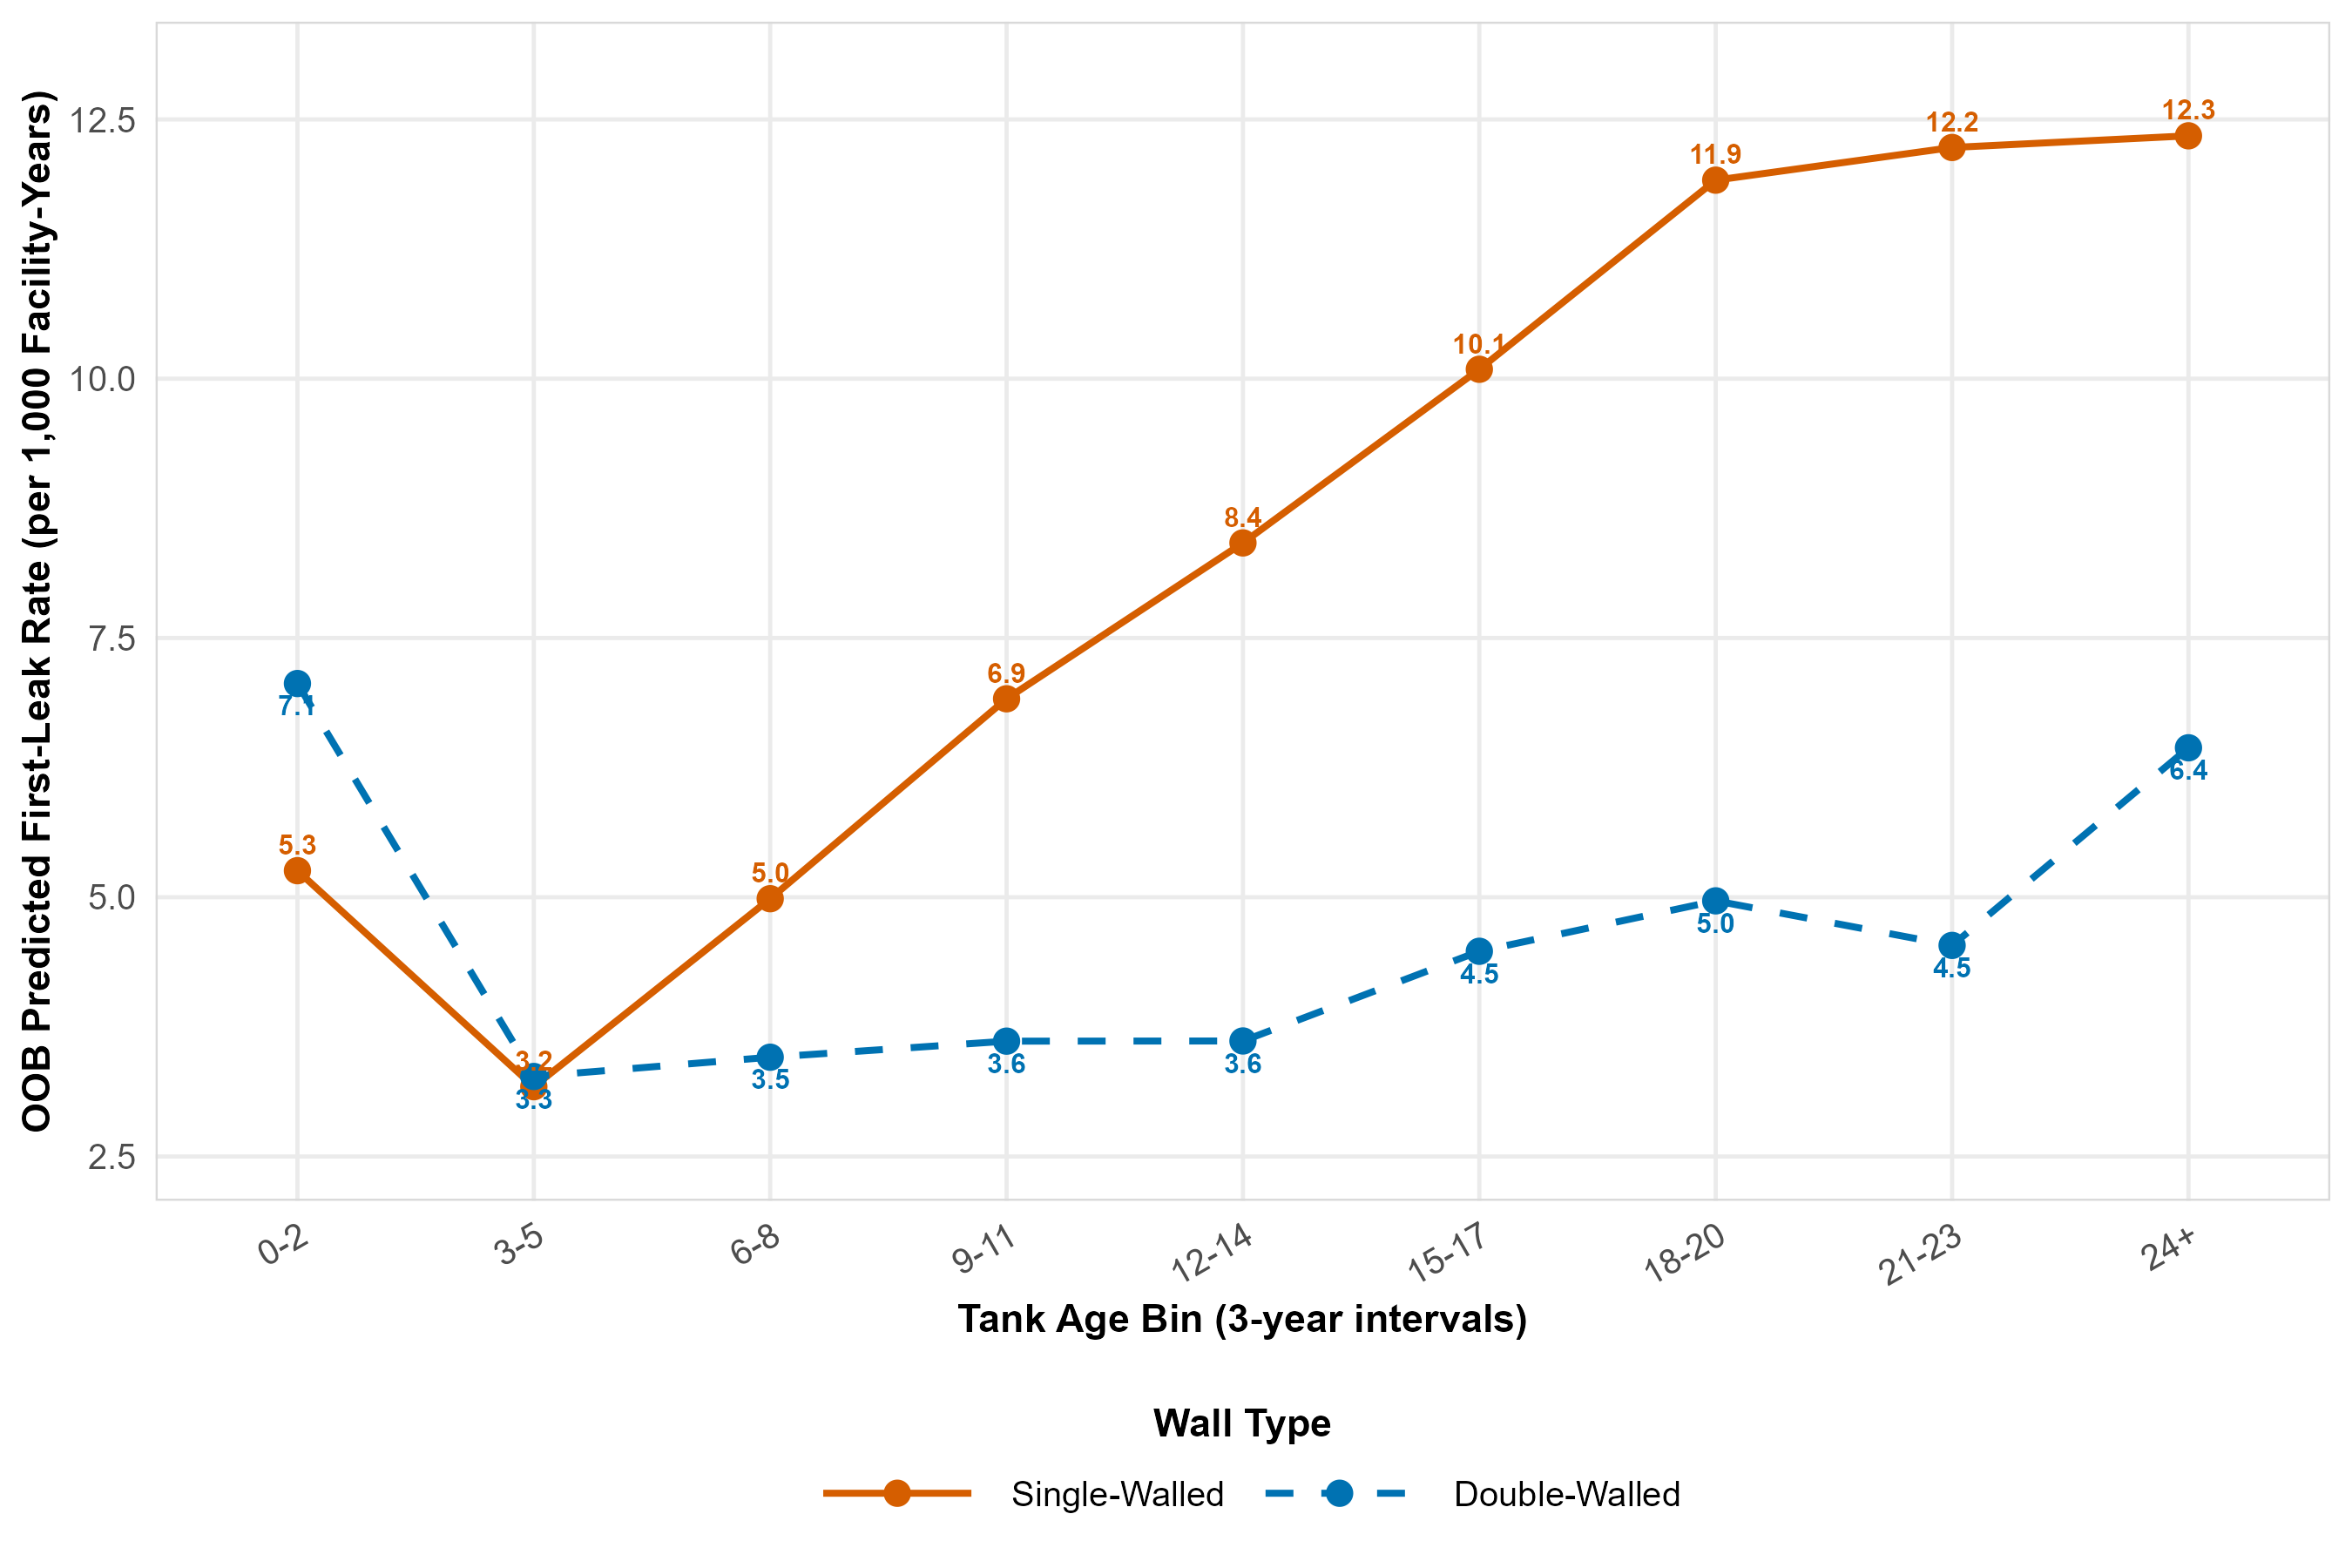
\includegraphics[width=0.92\textwidth,height=0.78\textheight,keepaspectratio]{../../Output/Figures/Figure_CV_CellRisk.png}
\end{center}

\begin{tikzpicture}[remember picture, overlay]
\node[anchor=south west, inner sep=0pt] at ([xshift=10pt, yshift=10pt]current page.south west) {%
  \navbutton[cell-gof][fill=BerkeleyBlue, font=\tiny, inner sep=2pt]{Goodness of fit $\rightarrow$}%
};
\end{tikzpicture}
\end{frame}

\begin{frame}{The insurance market: how Texas premiums are built}
\phantomsection\label{the-insurance-market-how-texas-premiums-are-built}
\BerkeleyLightMode

\textbf{Texas} --- rebuilt from marjor Texas UST Insurer's rate filings
(SERFF, 2006--2024):

\[P_{ijt} \;=\; \text{Base}_t \;\times\; \text{ILF}_{it} \;\times\; \Bigl(1 \;+\; \sum_{k} \lambda_{k,t}\, X_{ijt,k}\Bigr)\]

\begin{itemize}
\tightlist
\item
  \(\text{Base}_t\): per-tank base rate, four filing periods
\item
  \(\text{ILF}_{it}\): increased-limit factor; fix coverage at
  federal-minimum \$1M/\$1M
\item
  \(X_{ijt}\): tank age, wall, piping, leak-detection technology
\item
  \(\lambda_{k,t}\): additive credits/debits from the filed schedule
\end{itemize}

\textbf{Control states} --- state financial-responsibility fund records:
a per-tank annual assessment, largely flat across years and tank
characteristics.
\end{frame}

\begin{frame}{Premiums track the risk we can predict}
\phantomsection\label{premiums-track-the-risk-we-can-predict}
\BerkeleyLightMode

\vspace{0.1cm}
\begin{center}
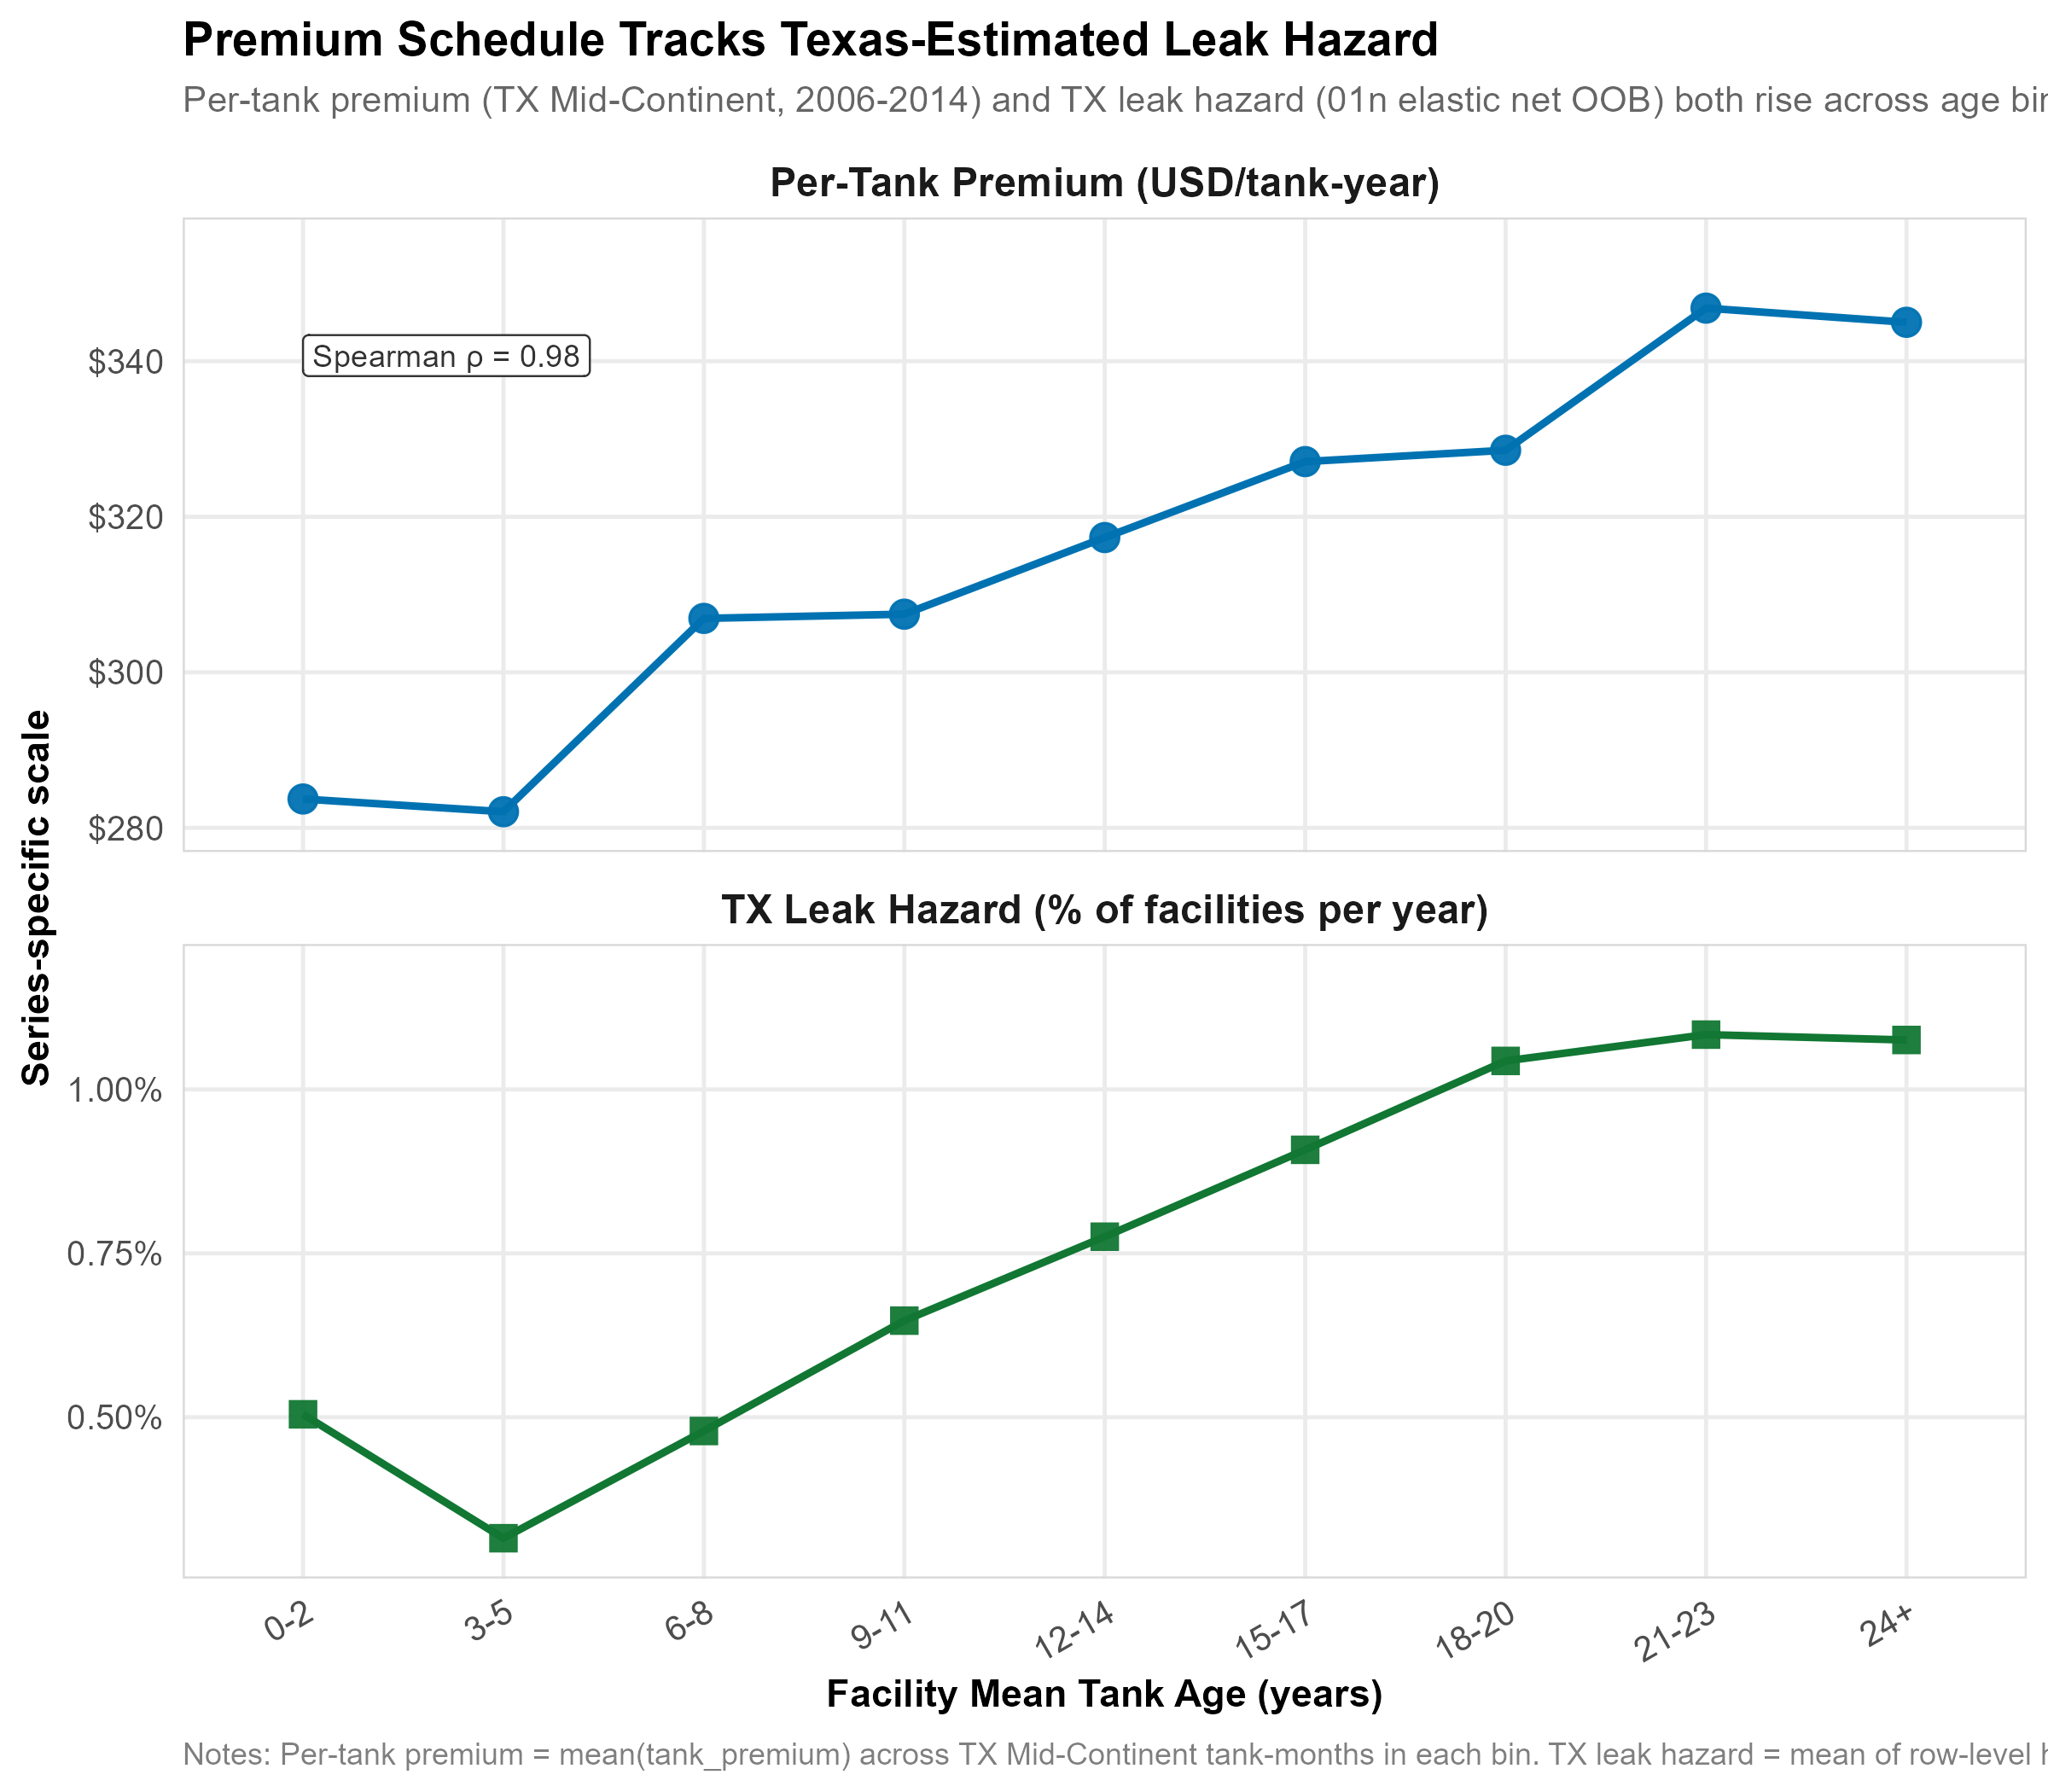
\includegraphics[height=0.80\textheight,keepaspectratio]{../../Output/Figures/Figure_Premium_vs_Hazard_Raw.png}
\end{center}

\begin{tikzpicture}[remember picture, overlay]
\node[anchor=south west, inner sep=0pt] at ([xshift=10pt, yshift=10pt]current page.south west) {%
  \navbutton[premium-vs-el][fill=BerkeleyBlue, font=\tiny, inner sep=2pt]{Predicted per-tank EL $\rightarrow$}%
};
\end{tikzpicture}
\end{frame}

\begin{frame}{Premium divergence: Texas vs.~control states (1992--2020)}
\phantomsection\label{premium-divergence-texas-vs.-control-states-19922020}
\BerkeleyLightMode

\vspace{0.2cm}
\begin{center}
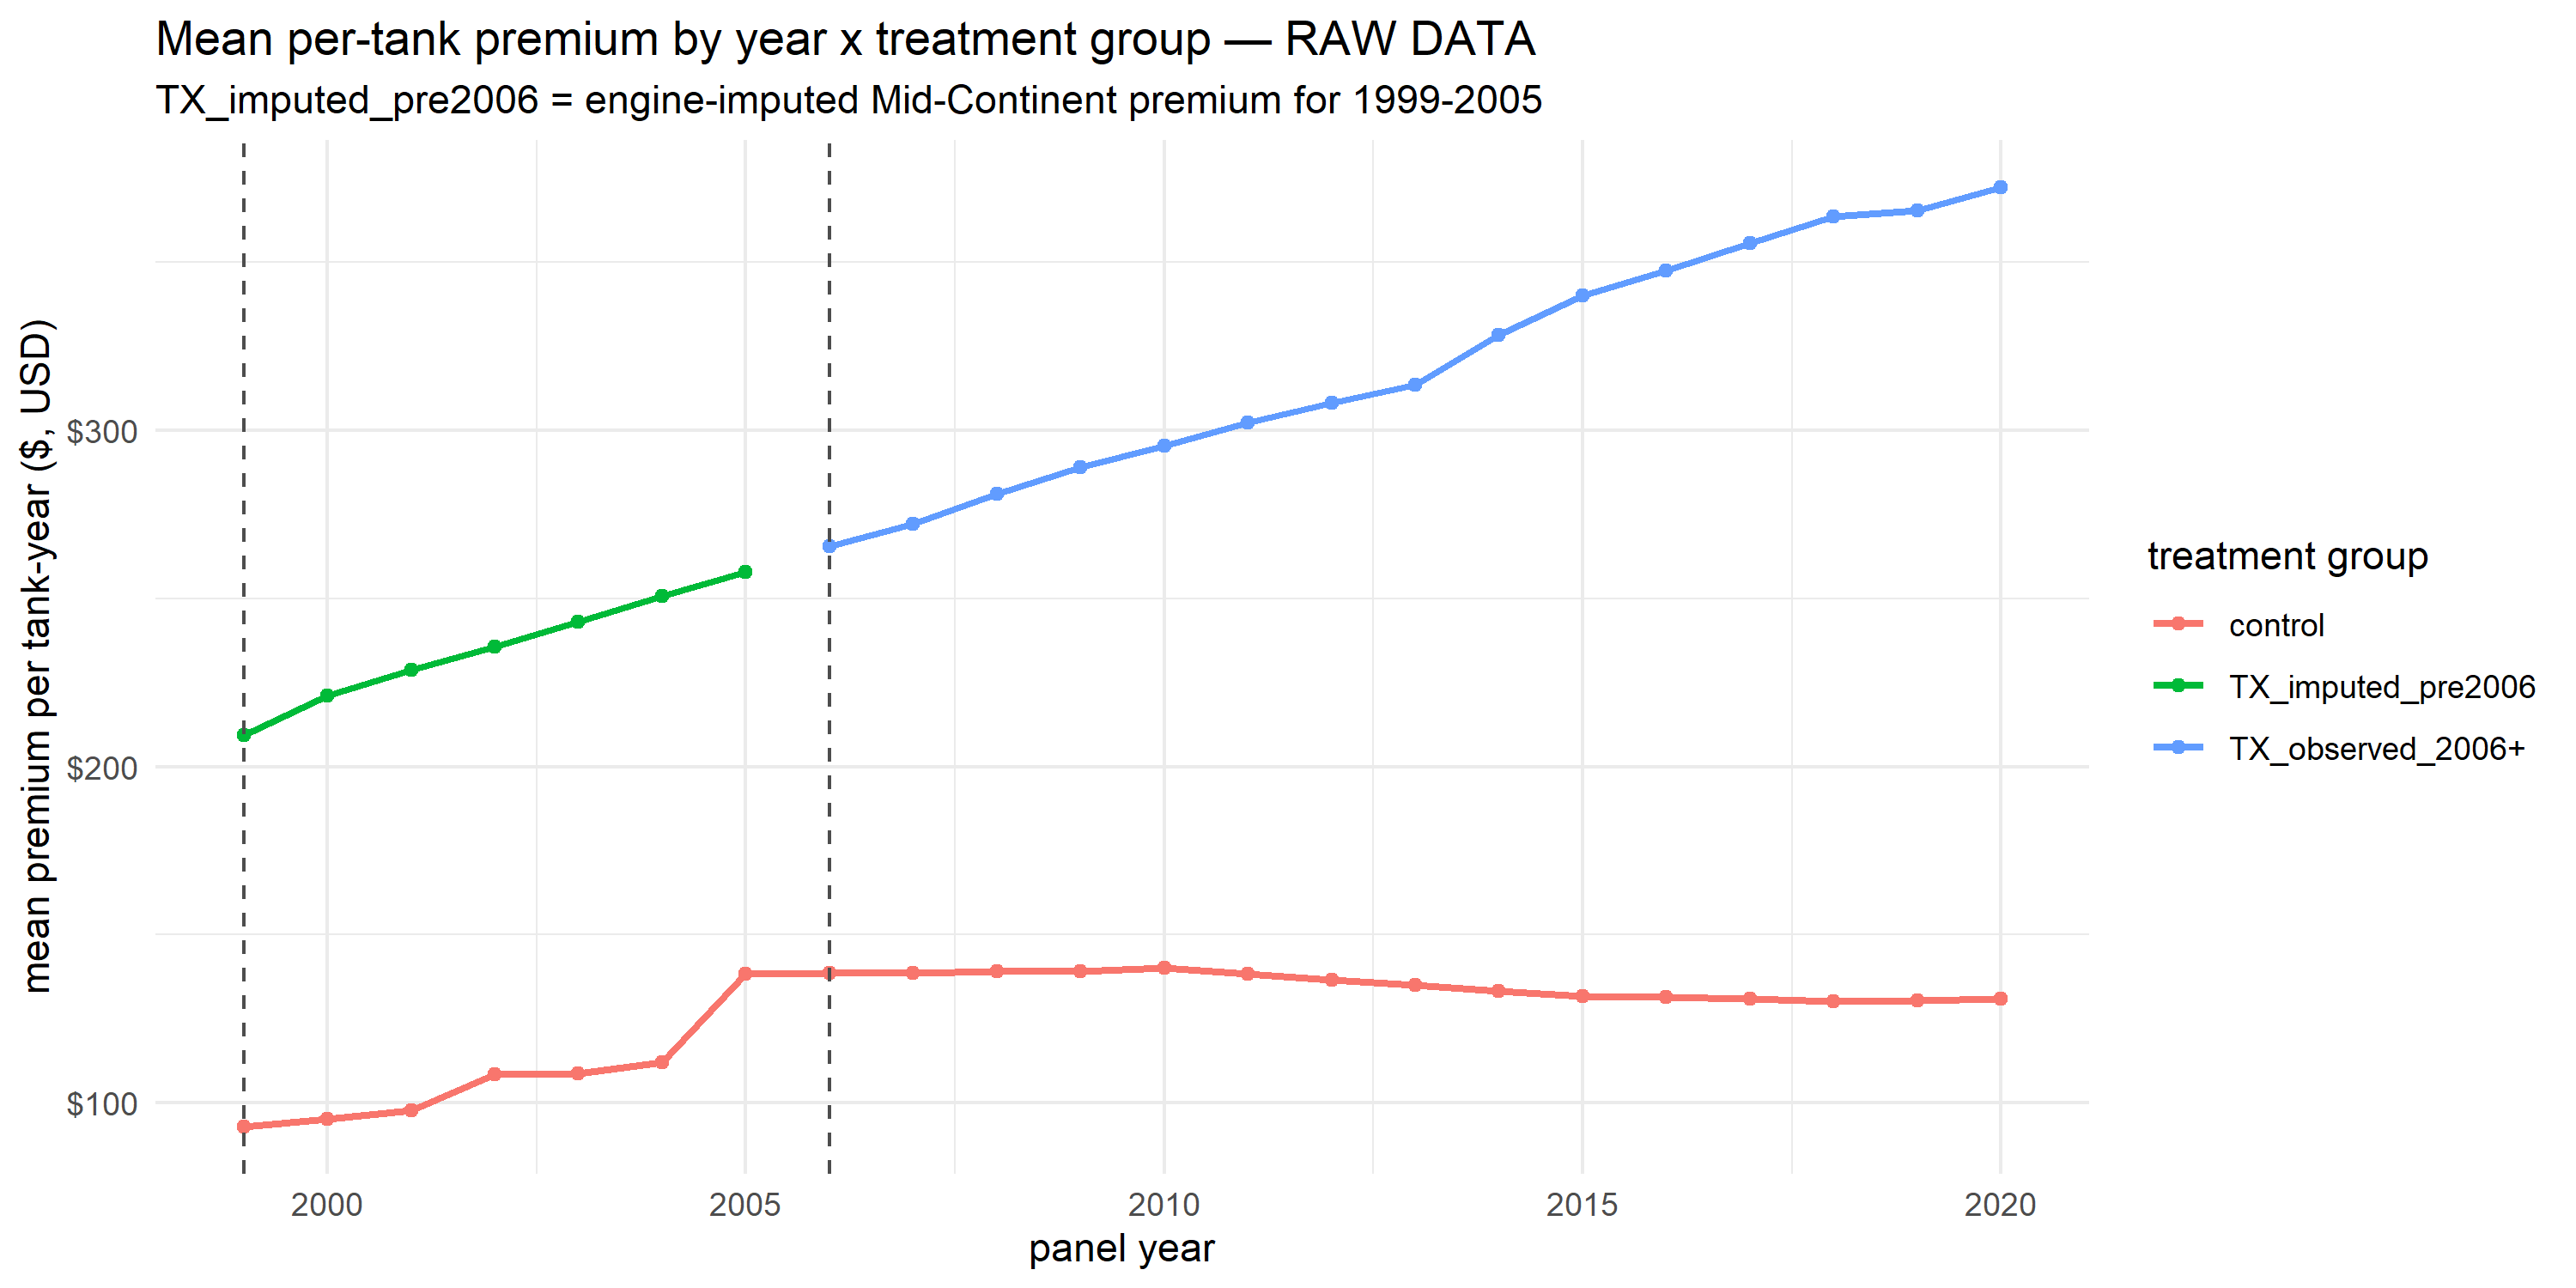
\includegraphics[width=0.92\textwidth,height=0.78\textheight,keepaspectratio]{../../Output/Figures/04e_Premium_by_Year_Treatment.png}
\end{center}

\vspace{0.1cm}

\centering\small\textit{Flat and parallel before 1998; sharp Texas divergence after the reform. Sets up the DiD without showing it.}
\end{frame}

\begin{frame}{}
\phantomsection\label{section-1}
\BerkeleyMode

\begin{center}
\Huge \textbf{Reduced Form Evidence}
\end{center}
\end{frame}

\begin{frame}{Research design: DiD with facility FE and cell-by-year FE}
\phantomsection\label{research-design-did-with-facility-fe-and-cell-by-year-fe}
\BerkeleyLightMode

\textbf{Static DiD.}

\[Y_{it} \;=\; \beta\,(\text{Texas}_{f(i)} \times \text{Post}_t) \;+\; \alpha_i \;+\; \delta_{ct} \;+\; \varepsilon_{it}\]

\textbf{Event study.}

\[Y_{it} \;=\; \sum_{\tau \neq -1} \beta_\tau \cdot \bigl(\text{Texas}_{f(i)} \times \mathbf{1}[t - 1998 = \tau]\bigr) \;+\; \alpha_i \;+\; \delta_{ct} \;+\; \varepsilon_{it}\]

\begin{itemize}
\tightlist
\item
  \(\alpha_i\): facility FE. \(\delta_{ct}\): cell\(\times\)year FE with
  \(c = \{\text{wall}\times\text{fuel}\times\text{capacity}\times\text{install cohort}\}\)
\item
  \emph{Identifying variation:} within a single tank-vintage cell, in
  the same calendar year, \(\beta\) is the change in the
  Texas-vs-control closure-rate gap before vs.~after Dec 22, 1998
\end{itemize}
\end{frame}

\begin{frame}{Event study: closure response in Texas}
\phantomsection\label{event-study-closure-response-in-texas}
\BerkeleyLightMode

\vspace{0.2cm}
\begin{center}
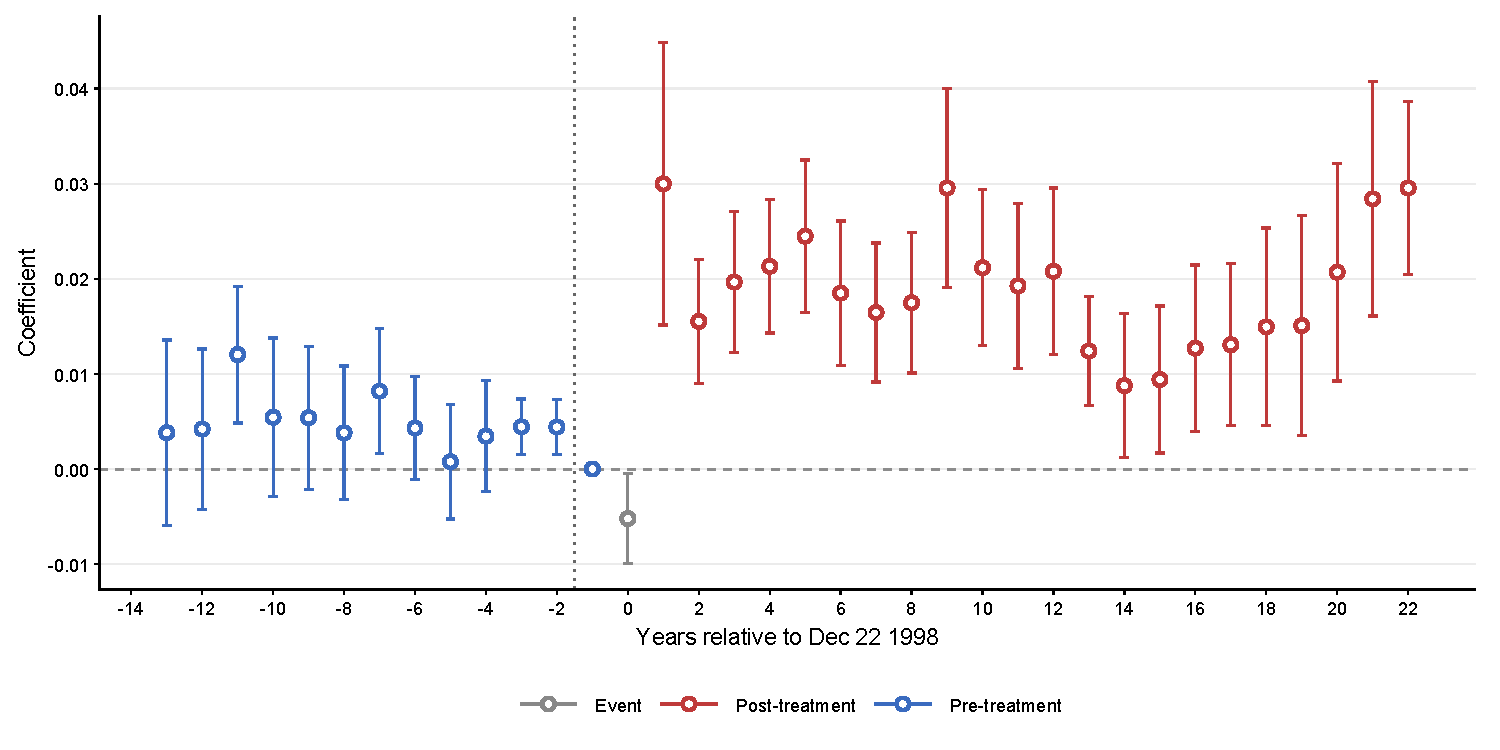
\includegraphics[width=0.92\textwidth,height=0.78\textheight,keepaspectratio]{../../Output/Figures/Fig_ES_Full.pdf}
\end{center}

\vspace{0.1cm}

\centering\small\textit{Pre-trends flat; sharp break at Dec 22, 1998; sustained post-treatment effect.}
\end{frame}

\begin{frame}{ATT on Tank Closure: \(+1.58\) pp on a \(2.0\%\) Baseline}
\phantomsection\label{att-on-tank-closure-1.58-pp-on-a-2.0-baseline}
\BerkeleyLightMode

\vspace{0.15cm}
\begin{center}
\begingroup
\scriptsize
\setlength{\tabcolsep}{5pt}
\renewcommand{\arraystretch}{0.95}

\begingroup
\centering
\begin{tabular}{lcccc}
   \toprule
                                            & (1) Raw        & (2) + Fac FE         & (3) + Controls & (4) + Cell FE \\   
                                            & (1)            & (2)                  & (3)            & (4)\\  
   \midrule 
   Constant                                 & 0.0203$^{***}$ &                      &                &   \\   
                                            & (0.0022)       &                      &                &   \\   
   did\_term                                & 0.0106$^{***}$ & 0.0338$^{***}$       & 0.0350$^{***}$ & 0.0158$^{***}$\\   
                                            & (0.0022)       & ($1\times 10^{-6}$)  & (0.0015)       & (0.0040)\\   
   mandate\_release\_det                    &                &                      & -0.0039        &   \\   
                                            &                &                      & (0.0035)       &   \\   
   mandate\_spill\_overfill                 &                &                      & 0.0048$^{*}$   &   \\   
                                            &                &                      & (0.0025)       &   \\   
   mandate\_integrity                       &                &                      & 0.0085$^{***}$ &   \\   
                                            &                &                      & (0.0026)       &   \\   
    \\
   Observations                             & 9,761,982      & 9,761,982            & 9,761,982      & 9,761,044\\  
   R$^2$                                    & 0.00047        & 0.03550              & 0.03584        & 0.07745\\  
   Within R$^2$                             &                & 0.00218              & 0.00253        & 0.00036\\  
    \\
   panel\_id fixed effects                  &                & $\checkmark$         & $\checkmark$   & $\checkmark$\\   
   cell\_vintage\_year\_fe fixed effects    &                &                      &                & $\checkmark$\\   
   \bottomrule
\end{tabular}
\par\endgroup



\endgroup
\end{center}

\vfill

\centering

\textit{Cols add facility FE, then cell$\times$year FE. Col (3) is the headline.}
\end{frame}

\begin{frame}{Heterogeneity: Pre-89 Vintage Drives the Effect}
\phantomsection\label{heterogeneity-pre-89-vintage-drives-the-effect}
\BerkeleyLightMode

\vspace{-0.1cm}
\begin{center}
\begingroup
\scriptsize
\setlength{\tabcolsep}{3pt}
\renewcommand{\arraystretch}{0.7}

\begingroup
\centering
\begin{tabular}{lcccc}
   \toprule
                                            & (1) Raw        & (2) + Fac FE   & (3) + Controls & (4) + Cell FE \\   
                                            & (1)            & (2)            & (3)            & (4)\\  
   \midrule 
   Constant                                 & 0.0103$^{***}$ &                &                &   \\   
                                            & (0.0011)       &                &                &   \\   
   did\_term                                & 0.0048$^{***}$ & 0.0117$^{***}$ & 0.0114$^{***}$ & -0.0067$^{**}$\\   
                                            & (0.0011)       & (0.0028)       & (0.0029)       & (0.0031)\\   
   pre89\_cohort                            & 0.0135$^{***}$ & 0.0671$^{***}$ & 0.0696$^{***}$ &   \\   
                                            & (0.0023)       & (0.0062)       & (0.0060)       &   \\   
   did\_term $\times$ pre89\_cohort         & 0.0094$^{***}$ & 0.0382$^{***}$ & 0.0360$^{***}$ & 0.0309$^{***}$\\   
                                            & (0.0023)       & (0.0029)       & (0.0029)       & (0.0065)\\   
   mandate\_release\_det                    &                &                & -0.0114$^{**}$ &   \\   
                                            &                &                & (0.0040)       &   \\   
   mandate\_spill\_overfill                 &                &                & 0.0009         &   \\   
                                            &                &                & (0.0028)       &   \\   
   mandate\_integrity                       &                &                & 0.0044         &   \\   
                                            &                &                & (0.0030)       &   \\   
    \\
   Observations                             & 9,761,982      & 9,761,982      & 9,761,982      & 9,761,044\\  
   R$^2$                                    & 0.00249        & 0.04685        & 0.04750        & 0.07772\\  
   Within R$^2$                             &                & 0.01392        & 0.01460        & 0.00065\\  
    \\
   panel\_id fixed effects                  &                & $\checkmark$   & $\checkmark$   & $\checkmark$\\   
   cell\_vintage\_year\_fe fixed effects    &                &                &                & $\checkmark$\\   
   \bottomrule
\end{tabular}
\par\endgroup



\endgroup
\end{center}

\centering\scriptsize

\textit{Pre-89 ATT $= \hat\beta_0 + \hat\beta_1 \approx +3.1$ pp; post-88 ATT $= \hat\beta_0 \approx +0.6$ pp.}

\begin{tikzpicture}[remember picture, overlay]
\node[anchor=south west, inner sep=0pt] at ([xshift=10pt, yshift=10pt]current page.south west) {%
  \navbutton[vintage-forest][fill=BerkeleyBlue, font=\tiny, inner sep=2pt]{ATT by install year $\rightarrow$}%
};
\end{tikzpicture}
\end{frame}

\begin{frame}{LUST discovery falls under risk-based pricing}
\phantomsection\label{lust-discovery-falls-under-risk-based-pricing}
\BerkeleyLightMode

\vspace{0.2cm}
\begin{center}
\begingroup
\footnotesize
\renewcommand{\arraystretch}{1.05}
\begin{tabular}{lcc}
\toprule
Outcome & Pre-reform ctrl mean & TX $\times$ Post \\
\midrule
Any leak found this year                       & 1.73\% & $-$1.27\,pp\textsuperscript{***} \\
                                               &        & (0.0032)                         \\
\midrule
\multicolumn{3}{l}{\textit{By how the leak was discovered:}}                                \\
\hspace{0.5em}Routine monitoring               & 1.16\% & $-$0.76\,pp\textsuperscript{***} \\
\hspace{0.5em}\textit{(no closure in $\pm$60d)}&        & (0.0021)                         \\
\hspace{0.5em}Closure-inspection finding       & 0.61\% & $-$0.51\,pp\textsuperscript{**}  \\
\hspace{0.5em}\textit{(closure within 60d)}    &        & (0.0017)                         \\
\midrule
$N$ facility-years & \multicolumn{2}{c}{4{,}650{,}240}                                                  \\
Sample             & \multicolumn{2}{c}{Incumbent (alive at Dec 22, 1998)}                             \\
FE                 & \multicolumn{2}{c}{Facility + cell $\times$ year; cluster by state}    \\
\bottomrule
\end{tabular}

\endgroup
\end{center}

\vspace{0.1cm}

\centering\small\textit{Leak discovery falls $1.27$ pp on a $1.73\%$ base; both routine-monitoring and closure-inspection findings decline.}

\begin{tikzpicture}[remember picture, overlay]
\node[anchor=south west, inner sep=0pt] at ([xshift=10pt, yshift=10pt]current page.south west) {%
  \navbutton[lust-es][fill=BerkeleyBlue, font=\tiny, inner sep=2pt]{LUST event study $\rightarrow$}%
};
\end{tikzpicture}
\end{frame}

\begin{frame}{Closure composition shifts toward replacement}
\phantomsection\label{closure-composition-shifts-toward-replacement}
\BerkeleyLightMode

\vspace{0.05cm}
\begin{center}
\begingroup
\let\small\scriptsize
\scriptsize
\renewcommand{\arraystretch}{0.85}
\small
\begin{tabular}{lcc}
\toprule
Outcome (conditional on closing) & Pre-reform ctrl mean & TX $\times$ Post \\
\midrule
Facility closes all tanks this year     & 70.9\%       & $+$6.5\,pp\textsuperscript{***} \\
                                        &              & (0.019)                          \\
Has a permanent closure (no replace)    & 88.3\%       & $-$6.2\,pp\textsuperscript{***} \\
                                        &              & (0.012)                          \\
Has a replacement closure (upgrade)     & 12.0\%       & $+$6.3\,pp\textsuperscript{***} \\
                                        &              & (0.013)                          \\
Any DW tank installed                   & 4.1\%        & $-$1.4\,pp\textsuperscript{*}   \\
                                        &              & (0.007)                          \\
Net tank change (count)                 & $-$1.905     & $+$0.020                         \\
                                        &              & (0.085)                          \\
Capacity change (gal)                   & $-$100{,}394 & $-$1{,}397                       \\
                                        &              & (5{,}715)                        \\
\midrule
$N$ closing facility-years & \multicolumn{2}{c}{59{,}107}                                                       \\
Sample                     & \multicolumn{2}{c}{Incumbent, any\_closure $=1$}                                   \\
FE                         & \multicolumn{2}{c}{Facility + make\_model\_fac $\times$ year; cluster by state}    \\
\bottomrule
\end{tabular}

\endgroup
\end{center}

\vspace{0.05cm}

\centering\scriptsize\textit{Among closing facilities, RBP raises the replacement (upgrade) share and lowers permanent closures --- the margin the structural model recovers.}
\end{frame}

\begin{frame}{What the reduced form cannot tell us}
\phantomsection\label{what-the-reduced-form-cannot-tell-us}
\BerkeleyLightMode

\textbf{The DiD identifies an average treatment effect. Three questions it cannot answer:}

\vspace{0.2cm}

\begin{enumerate}

\item \textbf{How large are the welfare effects in dollar terms?} The DiD gives us a closure-rate gap; it does not give us a present-value welfare number on which to compare policies.

\item \textbf{What would alternative policies --- subsidy, Pigouvian surcharge, age mandate --- actually do?} These policies were not implemented in Texas. Their welfare consequences are counterfactual.

\item \textbf{How far are we from first-best, and why?} RBP is a partial fix: premiums price what the insurer can claim, but health damages are structurally unpriced. Quantifying the residual wedge requires the structural primitives.

\end{enumerate}

\vfill

\textbf{Recovering the structural parameters ($\kappa$, $K$, $\gamma_p$, $\gamma_r$) is the only way to answer these. The structural model is not an add-on --- it is required.}
\end{frame}

\begin{frame}{}
\phantomsection\label{section-2}
\BerkeleyMode

\begin{center}
\Huge \textbf{Structural Model and Counterfactuals}
\end{center}
\end{frame}

\begin{frame}{A dynamic discrete-choice model of tank operations}
\phantomsection\label{a-dynamic-discrete-choice-model-of-tank-operations}
\BerkeleyLightMode

\begin{itemize}
\tightlist
\item
  Each period, a facility chooses one of three actions:
  \textbf{Maintain}, \textbf{Exit}, or \textbf{Replace}
\item
  The choice trades off current flow payoffs against the continuation
  value of future operation
\item
  Framework: optimal stopping (Rust 1987); estimated by Nested
  Pseudo-Likelihood (Aguirregabiria \& Mira 2007)
\end{itemize}

\begin{tikzpicture}[remember picture, overlay]
\node[anchor=south west, inner sep=0pt] at ([xshift=10pt, yshift=10pt]current page.south west) {%
  \navbutton[model-coding][fill=BerkeleyBlue, font=\tiny, inner sep=2pt]{How the model codes each action $\rightarrow$}%
};
\end{tikzpicture}
\end{frame}

\begin{frame}{Flow utilities: one payoff per action}
\phantomsection\label{flow-utilities-one-payoff-per-action}
\BerkeleyLightMode

\begin{align*}
u^M(s,g) &= \underbrace{1}_{\text{net rev.}} + \estc{\gamma_{\text{price}}}\,P(s) - \estc{\gamma_{\text{risk}}}\,h(s) + \alpha_g
  &&\text{\small(maintain)}\\[2pt]
u^E(s)   &= \estc{\kappa_{w(s)}} &&\text{\small(exit / scrap)}\\[2pt]
u^R(s,g) &= -\estc{K_{w(s)}} + \alpha_g &&\text{\small(replace)}
\end{align*}

\vspace{0.15cm}

\begin{itemize}
\tightlist
\item
  \(P(s)\) premium (SERFF filings), \(h(s)\) leak hazard (risk model)
  --- both vary by (age, wall, regime)
\item
  \textbf{Estimated} (in \estc{green}): \(\estc{\kappa_w}\) scrap value,
  \(\estc{K_w}\) replacement cost, \(\estc{\gamma_{\text{price}}}\)
  price sensitivity, \(\estc{\gamma_{\text{risk}}}\) risk
  internalization
\item
  \(\alpha_g\) state\(\times\)regime stay FE --- a measurement
  correction, profiled out; it does not enter the counterfactual
\end{itemize}

\vfill

\centering\small\textit{Net revenue $R$ normalized to \$10k/yr/facility; all values in this scale.}
\end{frame}

\begin{frame}{Keep, scrap, or replace: the dynamic stopping problem}
\phantomsection\label{keep-scrap-or-replace-the-dynamic-stopping-problem}
\BerkeleyLightMode

\[V(s) = \max \Bigl\{\; \underbrace{u^M(s) + \beta\,\mathbb{E}[V(s')\mid s]}_{\text{Maintain}}, \;\; \underbrace{\kappa_{w(s)}}_{\text{Exit}}, \;\; \underbrace{-K_{w(s)} + \beta\,\mathbb{E}[V(s_{\text{new}})]}_{\text{Replace}} \;\Bigr\}\]

\vspace{0.1cm}

\begin{itemize}
\tightlist
\item
  \textbf{Maintain} --- flow payoff today, keep the option to operate
  next year
\item
  \textbf{Exit} --- take \(\kappa_w\) and leave (absorbing)
\item
  \textbf{Replace} --- pay \(K_w\), restart with a new DW tank at age 0
\end{itemize}

\vspace{0.15cm}

\textbf{Regime.} Flat fees: premium flat in age \(\Rightarrow\) aging
carries no price penalty. Risk-based: premium rises with age
\(\Rightarrow\) continuation value falls \(\Rightarrow\) firms
exit/replace sooner.

\vfill

\centering\small\textit{Stopping rule: close once scrap value exceeds the value of continuing; RBP lowers the age at which that binds.}
\end{frame}

\begin{frame}{The same tank in two worlds}
\phantomsection\label{the-same-tank-in-two-worlds}
\BerkeleyLightMode

\textbf{A thought experiment.} Take one tank --- 28 years old,
single-walled, same leak risk in either world --- and drop it into each
pricing regime:

\vspace{0.3cm}

\begin{center}
\large
\renewcommand{\arraystretch}{1.3}
\begin{tabular}{lcc}
\toprule
 & \textbf{Flat-fee world} & \textbf{Risk-based world} \\
 & \small (control state) & \small (Texas) \\
\midrule
Annual premium       & \$130 (flat)  & \alert{\$380} (rises with age) \\
Leak risk $h(s)$     & high          & high \emph{(same)} \\
\midrule
$\Rightarrow$ closes the tank & sometimes & \alert{much more often} \\
\bottomrule
\end{tabular}
\end{center}

\vspace{0.3cm}

\begin{itemize}
\tightlist
\item
  It already closes \emph{sometimes} under flat fees --- that response
  to \textbf{risk alone} is \(\gamma_{\text{risk}}\)
\item
  The \alert{extra} closing once the premium jumps, risk unchanged, is
  \(\gamma_{\text{price}}\)
\end{itemize}

\vfill

\centering\small\textit{Same tank, same risk --- only the premium differs. The within-regime response gives risk; the across-regime gap gives price.}
\end{frame}

\begin{frame}{D \(\times\) hazard: the variation that identifies the
\(\gamma\)'s}
\phantomsection\label{d-times-hazard-the-variation-that-identifies-the-gammas}
\BerkeleyLightMode

\vspace{0.1cm}
\begin{center}
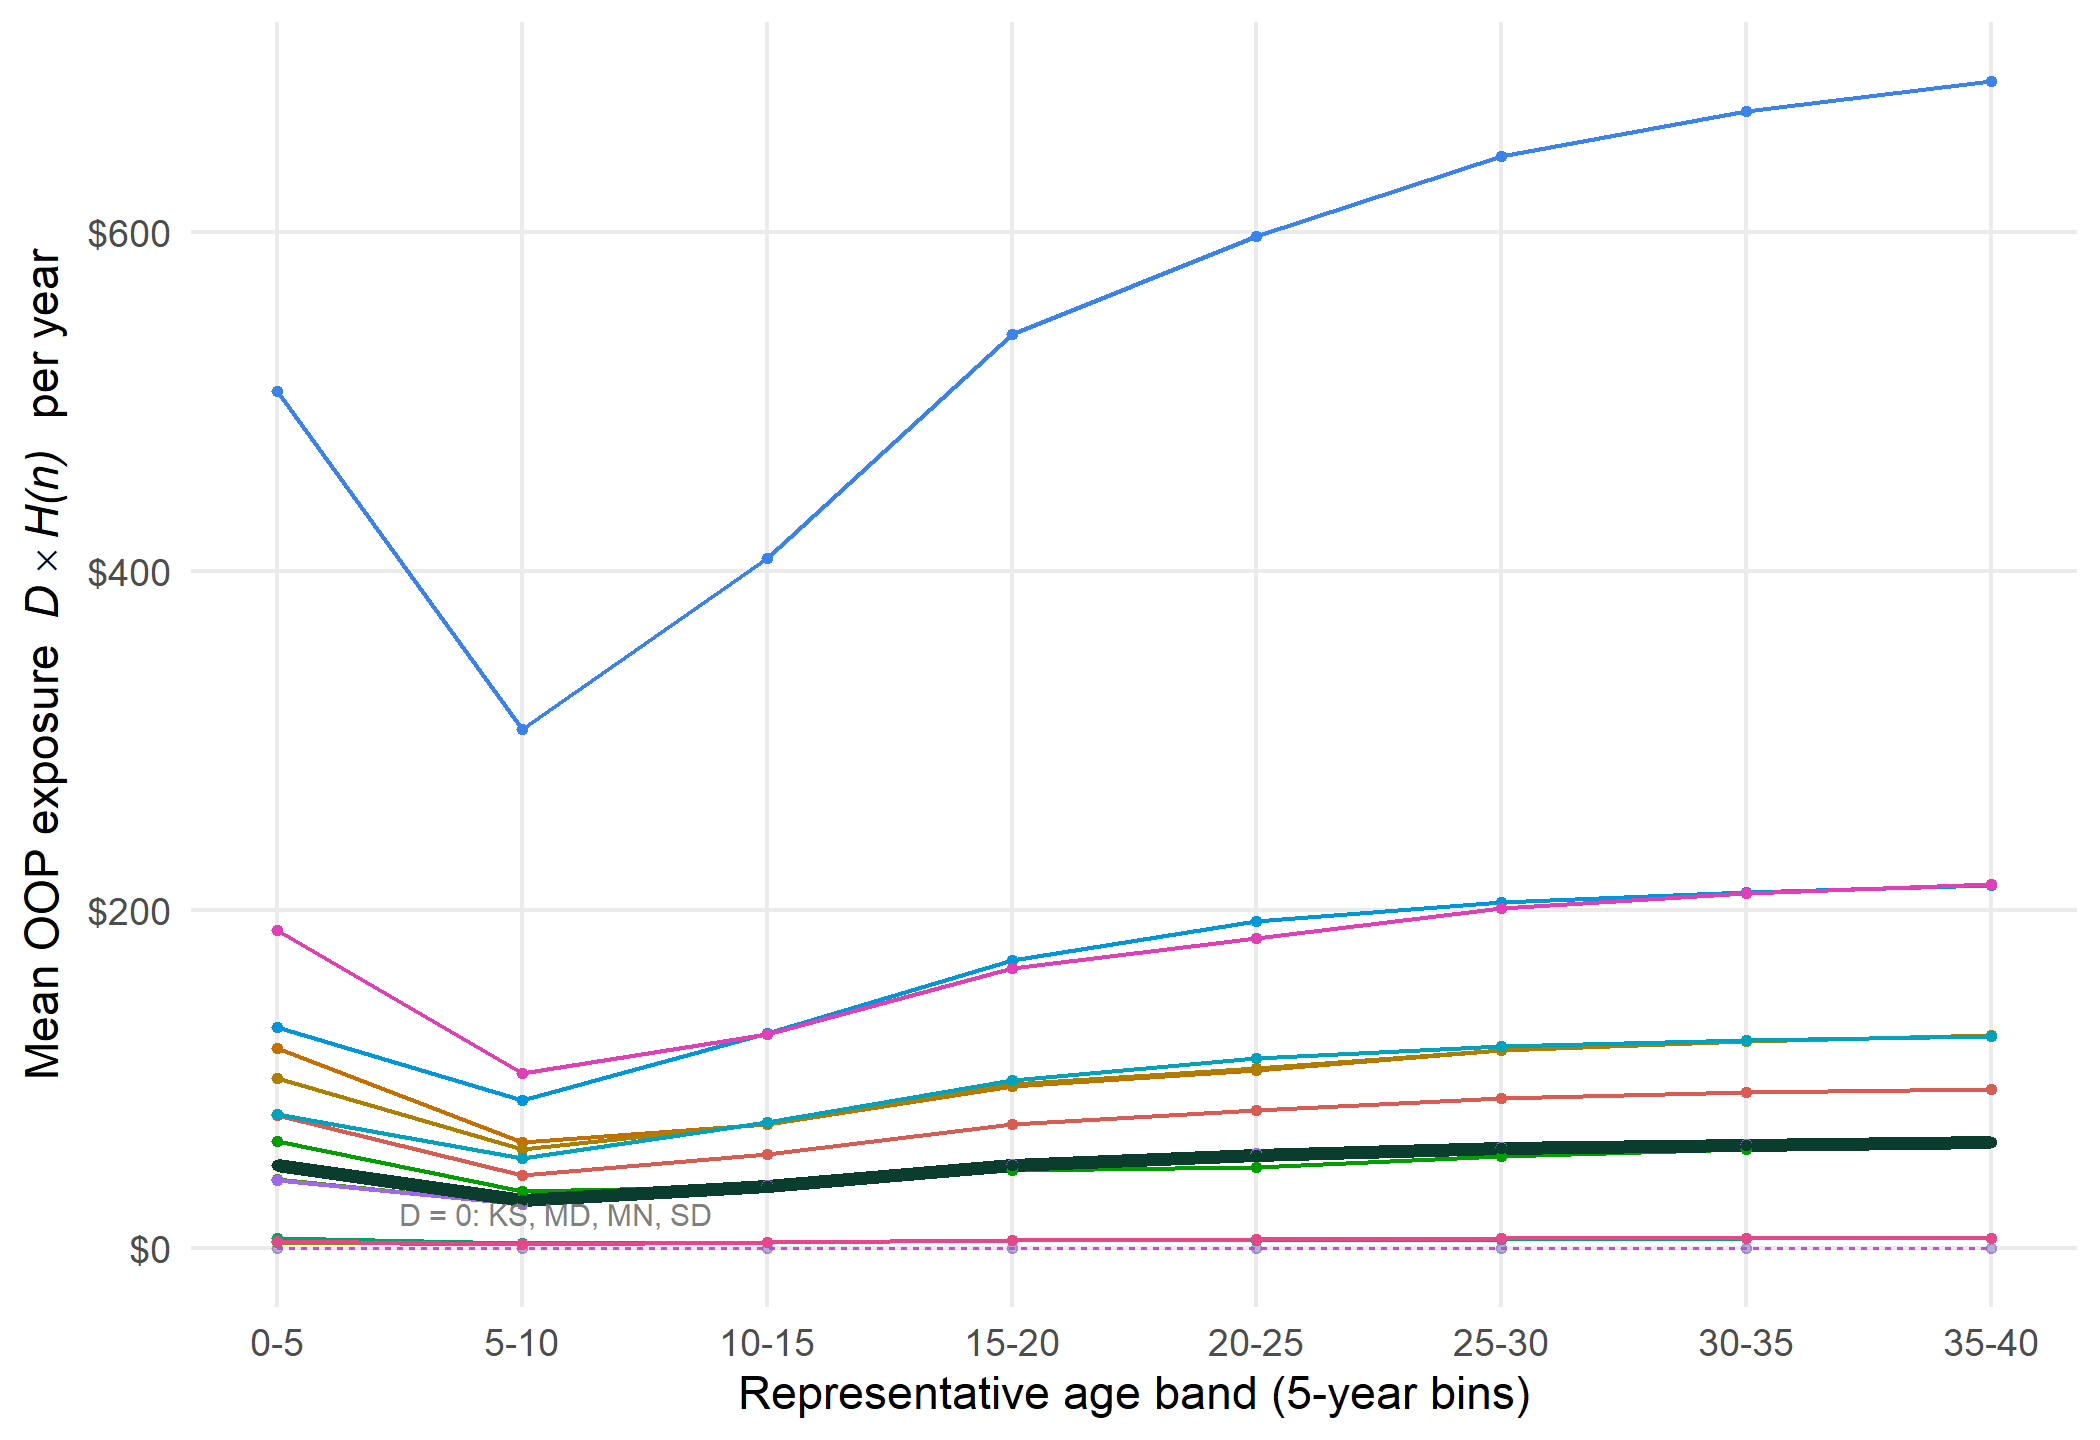
\includegraphics[width=0.92\textwidth,height=0.74\textheight,keepaspectratio]{../../Output/Figures/AE09_OOP_by_Age_Pooled.png}
\end{center}

\vspace{0.05cm}

\centering\small\textit{Flat-fee cells (orange) sit at low deductibles across the hazard range; risk-based cells (teal) price the hazard. Deductible variation at given hazard pins $\gamma_{\text{price}}$; the hazard spread pins $\gamma_{\text{risk}}$.}
\end{frame}

\begin{frame}{What identifies each parameter}
\phantomsection\label{what-identifies-each-parameter}
\BerkeleyLightMode

\hypertarget{identif-main}{}

\vspace{0.2cm}

\begin{center}
\normalsize
\renewcommand{\arraystretch}{1.5}
\begin{tabular}{p{2.8cm}p{8.5cm}}
\hline
\textbf{Parameter} & \textbf{Moment in the data} \\
\hline
$\kappa_{SW},\,\kappa_{DW}$ & Exit rate by wall type --- higher scrap value $\Rightarrow$ more exit \\
$K_{SW},\,K_{DW}$ & Replace-vs-exit share among closing facilities, by wall \\
$\gamma_{\text{price}}$ & Choice-share response to premium variation across cells \\
$\gamma_{\text{risk}}$ & Residual age--exit gradient once premium is accounted for \\
$\alpha_g$ & Group-level stay rate (profiled out --- measurement only) \\
\hline
\end{tabular}
\end{center}

\vfill

\centering\small\textit{The cross-regime contrast (FF: only hazard varies; RB: both vary) is what separates $\gamma_{\text{price}}$ from $\gamma_{\text{risk}}$.}

\begin{tikzpicture}[remember picture, overlay]
\node[anchor=south west, inner sep=0pt] at ([xshift=10pt, yshift=10pt]current page.south west) {%
  \navbutton[identif-exit][fill=BerkeleyBlue, font=\tiny, inner sep=2pt]{$\kappa$ exit share $\rightarrow$}%
  \hspace{3pt}%
  \navbutton[identif-replace][fill=BerkeleyBlue, font=\tiny, inner sep=2pt]{$K$ replace share $\rightarrow$}%
};
\end{tikzpicture}
\end{frame}

\begin{frame}{Structural estimating sample}
\phantomsection\label{structural-estimating-sample}
\BerkeleyLightMode

\textbf{Unit of observation.} Facility-year. One row per facility per
year, 1999--2018.

\textbf{Sample.} Texas 2006+ (post-RB implementation) plus 17 control
states 1999+. The structural model fits the \emph{equilibrium} of the
risk-based regime --- TX is the regime that's actually priced.

\begin{itemize}
\tightlist
\item
  N \(\approx\) 2.28M facility-years after data cleaning
\item
  Choices observed: maintain / exit / replace; mapped onto 32 state
  cells \((a, W, R)\)
\item
  Premiums \(p_t\) from Mid-Continent rate-filing reconstruction;
  hazards \(h(a_t)\) from the first-release-prediction model
\end{itemize}
\end{frame}

\begin{frame}{Parameter estimates: 6-parameter NPL with profiled state
FE}
\phantomsection\label{parameter-estimates-6-parameter-npl-with-profiled-state-fe}
\BerkeleyLightMode

\vspace{0.05cm}
\begin{center}
\footnotesize
\setlength{\tabcolsep}{10pt}
\renewcommand{\arraystretch}{0.88}
\begin{tabular}{lc}
\toprule
 & \textbf{Estimate} \\
\midrule
$\hat{\kappa}_{SW}$ \;\, scrap value, single-walled   & \$252{,}349 \\
                                                      & (\$1{,}213) \\
$\hat{\kappa}_{DW}$ \;\, scrap value, double-walled   & \$243{,}800 \\
                                                      & (\$1{,}239) \\
$\hat{K}_{SW}$ \;\, replacement cost, single-walled   & \$51{,}383 \\
                                                      & (\$176) \\
$\hat{K}_{DW}$ \;\, replacement cost, double-walled   & \$51{,}162 \\
                                                      & (\$372) \\
$\hat{\gamma}_{\text{price}}$ \;\, price sensitivity   & $-2.163$ \\
                                                      & $(0.205)$ \\
$\hat{\gamma}_{\text{risk}}$ \;\, risk internalization & $+0.114$ \\
                                                      & $(0.005)$ \\
\midrule
Log-likelihood            & $-227{,}240$ \\
Facility-years            & $2{,}282{,}735$ \\
State stay fixed effects  & $18$ \\
\bottomrule
\end{tabular}
\end{center}

\vspace{0.05cm}

\centering\scriptsize\textit{Standard errors in parentheses (Aguirregabiria--Mira 2002 profile likelihood). $\kappa$ and $K$ in dollars; $K$ standard errors via the delta method on the log scale. Both $\gamma$ are highly significant ($t=-10.6$ and $21.6$).}
\end{frame}

\begin{frame}{What the estimates say}
\phantomsection\label{what-the-estimates-say}
\BerkeleyLightMode

\vspace{0.2cm}

\begin{itemize}
\item
  \textbf{\(\hat\kappa_{SW}\approx\$252\)k,
  \(\hat\kappa_{DW}\approx\$244\)k.} Scrap value on exit --- close
  across wall types after the cleanup.
\item
  \textbf{\(\hat K_{SW}\approx\hat K_{DW}\approx\$51\)k.} New-tank cost
  barely moves with wall type --- wall matters through hazard and
  premium, not installation.
\item
  \textbf{\(\hat\gamma_{\text{price}}=-2.16\).} Firms respond strongly
  to the premium signal: higher premiums push toward exit and
  replacement.
\item
  \textbf{\(\hat\gamma_{\text{risk}}=+0.114\), small.} Firms act on only
  a sliver of expected leak damage --- most is externalized.
  \textbf{That wedge is what the counterfactuals quantify.}
\end{itemize}

\begin{tikzpicture}[remember picture, overlay]
\node[anchor=south west, inner sep=0pt] at ([xshift=10pt, yshift=10pt]current page.south west) {%
  \navbutton[fit-sw][fill=BerkeleyBlue, font=\tiny, inner sep=2pt]{Model fit $\rightarrow$}%
};
\end{tikzpicture}
\end{frame}

\begin{frame}{Each policy changes one term in the payoff}
\phantomsection\label{each-policy-changes-one-term-in-the-payoff}
\BerkeleyLightMode

\small

\textbf{Baseline (risk-based):}\quad \(u^M(s) = 1 + \gamma_{\text{price}}\,P(s) - \gamma_{\text{risk}}\,h(s) + \alpha_g\)

\vspace{0.18cm}

\textbf{CF1 --- Flat-fee:}\quad \(u^M(s) = 1 + \gamma_{\text{price}}\,\alert{\bar{P}} - \gamma_{\text{risk}}\,h(s)\)

\vspace{0.18cm}

\textbf{CF2 --- Replacement subsidy:}\quad \(u^R(s) = -\,\alert{(1 - s^*)}\,K_w,\quad \alert{s^* = 0.50}\)

\vspace{0.18cm}

\textbf{CF3 --- Pigouvian:}\quad \(u^M(s) = 1 + \gamma_{\text{price}}\,P(s) - \gamma_{\text{risk}}\,h(s) \;\alert{-\; h(s)\,E}\)

\vspace{0.18cm}

\textbf{CF4 --- Age mandate:}\quad \(u^M(s) = \alert{-\infty}\) ;, for
tanks \(25+\) years old

\vfill

\centering\small\textit{Each policy re-solves $V$ and the stationary fleet; only the \alert{highlighted} term moves.}
\end{frame}

\begin{frame}{Welfare accounting}
\phantomsection\label{welfare-accounting}
\BerkeleyLightMode

\vspace{0.4cm}

\[\Delta W = \underbrace{\sum_s \pi(s)\,\Delta V(s)}_{\Delta\text{ Firm surplus}} \;-\; \underbrace{\sum_s \pi(s)\sum_t \beta^t h(s_t)\,(L+E)}_{\Delta\text{ External damage}} \;-\; \underbrace{\Delta\text{Govt outlay}}_{\text{subsidy only}}\]

\vspace{0.4cm}

\begin{itemize}
\tightlist
\item
  \textbf{Firm surplus} --- change in the discounted value to operators
\item
  \textbf{External damage} --- unpriced cleanup \(+\) health harm,
  \(L+E\) per expected release
\item
  \textbf{Govt outlay} --- subsidy cost (CF2 only)
\end{itemize}

\vfill

\centering\small\textit{$E=\$17$k (health) or \$50k (with unmeasured damages). State fixed effects do not enter the counterfactual re-solve.}

\begin{tikzpicture}[remember picture, overlay]
\node[anchor=south west, inner sep=0pt] at ([xshift=10pt, yshift=10pt]current page.south west) {%
  \navbutton[portfolio-summary][fill=BerkeleyBlue, font=\tiny, inner sep=2pt]{Model vs.\ data: the limitation $\rightarrow$}%
};
\end{tikzpicture}
\end{frame}

\begin{frame}{Counterfactual welfare: change in firm surplus, external
damage, and outlay}
\phantomsection\label{counterfactual-welfare-change-in-firm-surplus-external-damage-and-outlay}
\BerkeleyLightMode

\vspace{0.1cm}
\begin{center}
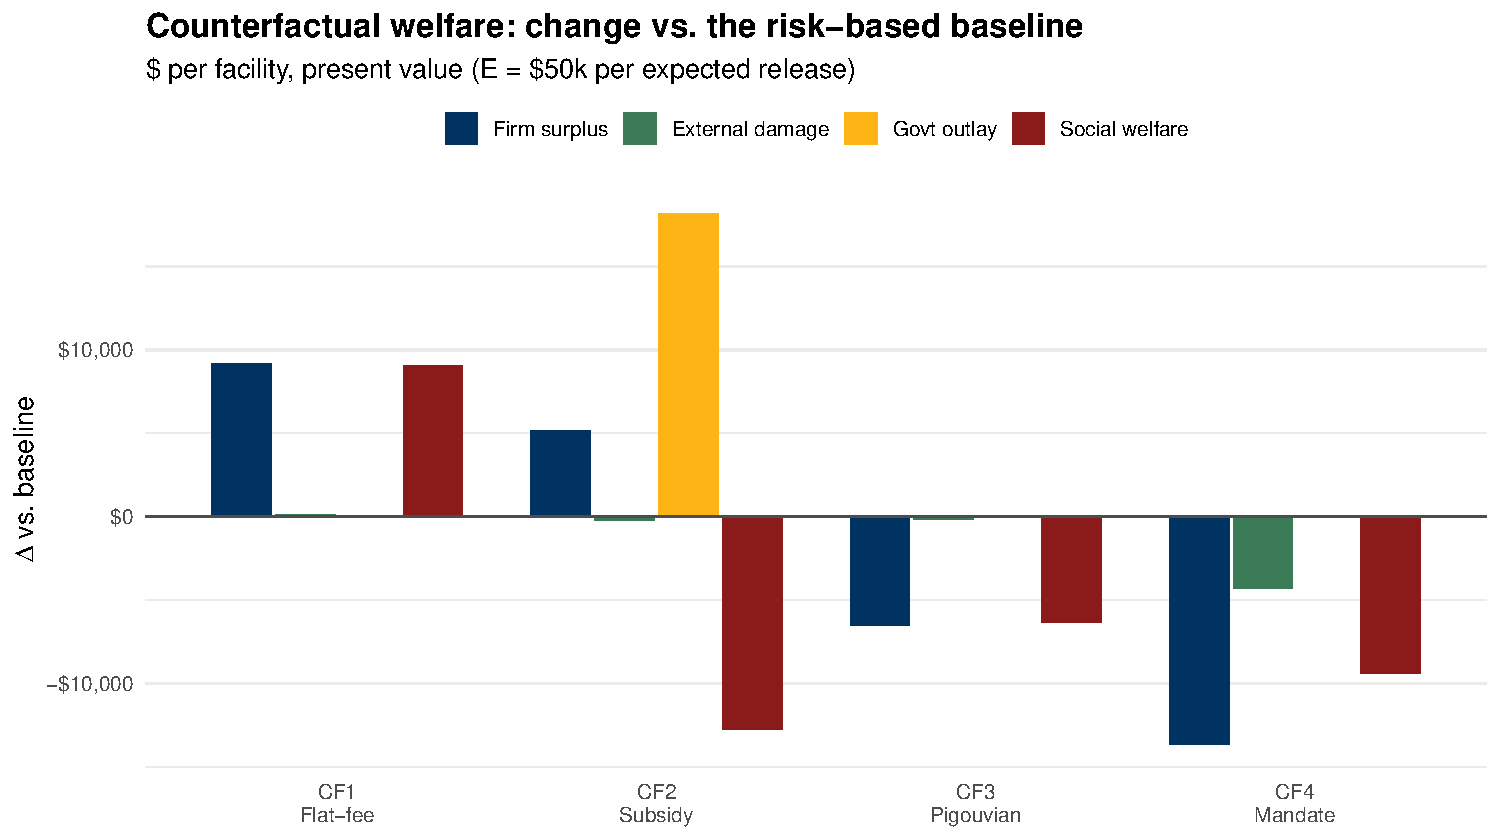
\includegraphics[width=0.95\textwidth,height=0.72\textheight,keepaspectratio]{../../Output/Figures/04v_Welfare_BarChart_Clean.pdf}
\end{center}

\vspace{0.1cm}

\centering\small\textit{Change in each welfare component relative to the risk-based baseline, by counterfactual ($\$$/facility, present value, $E=\$50$k). Bars above zero improve on the baseline.}
\end{frame}

\begin{frame}{Counterfactual welfare summary}
\phantomsection\label{counterfactual-welfare-summary}
\BerkeleyLightMode

\vspace{0.3cm}
\begin{center}
\small
\renewcommand{\arraystretch}{1.25}
\begin{tabular}{lrrrr}
\toprule
\textbf{Counterfactual} & \textbf{$\Delta$Firm} & \textbf{$\Delta$External} & \textbf{$\Delta$Govt} & \textbf{$\Delta$Social} \\
                        & \textbf{surplus}      & \textbf{damage}          & \textbf{outlay}        & \textbf{welfare}        \\
\midrule
CF1 --- Flat-fee        & $+9{,}213$  & $+120$     & $0$         & $+9{,}092$  \\
CF2 --- Replace subsidy & $+5{,}148$  & $-261$     & $+18{,}170$ & $-12{,}761$ \\
CF3 --- Pigouvian       & $-6{,}521$  & $-194$     & $0$         & $-6{,}327$  \\
CF4 --- Age mandate     & $-13{,}686$ & $-4{,}297$ & $0$         & $-9{,}389$  \\
\bottomrule
\end{tabular}
\end{center}

\vfill

\centering\small\textit{$\Delta$ vs. the risk-based baseline; $\$$/facility present value, $E=\$50$k. Positive = improvement over the baseline.}
\end{frame}

\begin{frame}{Takeaways}
\phantomsection\label{takeaways}
\BerkeleyLightMode

\begin{enumerate}
\item
  \textbf{Risk is observable.} The age-hazard gradient is steep for
  single-walled tanks and flat for double-walled. Shavell's
  observability condition is satisfied in this market.
\item
  \textbf{Risk-based pricing shifts behavior.} \(+1.58\) pp annual
  closure ATT; \(\sim\),4× larger in the pre-1989 SW-heavy stock that
  the premium schedule actually prices. Composition shifts toward the
  replacement margin (12\% → 18\%). LUST discovery falls through both
  background and inspection-triggered channels.
\item
  \textbf{Welfare gap to first-best persists.} {[}PLACEHOLDER:
  directional claim about the four counterfactuals at \(E = \$17\)k,
  pending 6p re-run. Even after the reform, the health-externality
  component remains structurally unpriced --- actuarial premiums cannot
  price what no claimant recovers.{]}
\end{enumerate}
\end{frame}

\begin{frame}{Appendix: The Agent's Decision (toy model)}
\phantomsection\label{appendix-the-agents-decision-toy-model}
\BerkeleyLightMode

\hypertarget{toy-agent}{}

\textbf{The Choice.} Each period \(t\), the facility chooses
\(d_t \in \{\text{Maintain}, \text{Close}\}\).

\textbf{The Trade-off.}

\begin{itemize}
\tightlist
\item
  \textbf{Maintain:} Earn net revenue, pay insurance premiums.
\item
  \textbf{Close:} Exit and recover scrap value \(\kappa\) (liquidity of
  land).
\end{itemize}

\textbf{Flow Utility (Maintain).}

\[
u(a) = \underbrace{R}_{\text{Net Revenue}} - \underbrace{C_j(a)}_{\text{Insurance Premium}}
\]

\emph{Simplifying assumption (full coverage):} environmental risk enters
as an \emph{ex-ante} premium cost, not an \emph{ex-post} shock.

\vspace{0.2cm}

\centering\small\textit{Two-action stopping model used in early presentations --- included for completeness; superseded by the three-action DCC in the main deck.}
\end{frame}

\begin{frame}{Appendix: The Dynamic Problem (toy model)}
\phantomsection\label{appendix-the-dynamic-problem-toy-model}
\BerkeleyLightMode

\hypertarget{toy-dynproblem}{}

\textbf{Bellman equation.}

\[
V(a) = \max \Bigl\{\, \underbrace{u(a) + \beta\, \mathbb{E}[V(a') \mid a]}_{\text{value of maintaining}}, \;\; \underbrace{\kappa}_{\text{scrap value}}\,\Bigr\}
\]

\textbf{Continuation value.} The value of keeping the tank active today
to preserve the option of operating tomorrow:

\[
V_{\text{cont}}(a) = u(a) + \beta\, \mathbb{E}[V(a') \mid a]
\]

\textbf{Optimal stopping rule.} Close if
\(V_{\text{cont}}(a) < \kappa\).
\end{frame}

\begin{frame}{Appendix: The Policy Lever: Insurance Regimes (toy model)}
\phantomsection\label{appendix-the-policy-lever-insurance-regimes-toy-model}
\BerkeleyLightMode

\hypertarget{toy-policylever}{}

\textbf{1. Uniform Premium Pooling (\(F\)) --- 38 states.}

\begin{itemize}
\tightlist
\item
  Premium: constant \(\bar P\), regardless of age or risk.
\item
  Marginal cost of aging: \(\;\partial C / \partial a = 0\). No
  incentive to close aging tanks.
\end{itemize}

\textbf{2. Risk-Based Pricing (\(RB\)) --- Texas post-1999.}

\begin{itemize}
\tightlist
\item
  Premium: rises with the leak hazard,
  \(C(a) = \lambda \cdot h(a) \cdot L\).
\item
  Marginal cost of aging: \(\;\partial C / \partial a > 0\). Aging tanks
  become increasingly costly.
\end{itemize}
\end{frame}

\begin{frame}{Appendix: What's the First Best? (toy model)}
\phantomsection\label{appendix-whats-the-first-best-toy-model}
\BerkeleyLightMode

\hypertarget{toy-firstbest}{}

\textbf{Social planner's objective.} Internalize remediation costs
(\(L\)) \emph{and} health externalities (\(E\)):

\[
u_{\text{SOC}}(a) = R - h(a) \cdot (\underbrace{L}_{\text{Remediation}} + \underbrace{E}_{\text{Health}})
\]

\textbf{Why risk-based pricing falls short.}

\begin{itemize}
\tightlist
\item
  Actuarial premiums reflect insurer claims data \(\rightarrow\) only
  remediation costs (\(L\))
\item
  Health damages (\(E\)) generate no third-party claims: contamination
  is unobservable (Marcus, 2021)
\item
  \(\Rightarrow\) Even fair risk-based pricing leaves \(E\) externalized
\end{itemize}

\textbf{Implication.} \(V_{\text{RB}}(a) > V_{\text{SOC}}(a)\) --- RBP
induces \emph{some} closures, but not enough.
\end{frame}

\begin{frame}{Appendix: Three Facts to Keep in Mind (toy model)}
\phantomsection\label{appendix-three-facts-to-keep-in-mind-toy-model}
\BerkeleyLightMode

\hypertarget{toy-threefacts}{}

\textbf{1. Asset depreciation.} Rising leak risk drives tank value
strictly down in age (\(V'(a) < 0\)). The regime determines whether
private incentives align with this social decay.

\textbf{2. Inefficient retention (Uniform Premium).} Static costs
\(\bar P\) imply zero marginal cost of aging. Firms ignore risk and
retain assets longest: \(a^*_{\text{UP}}\).

\textbf{3. Partial correction (Risk-Based).} Rising premiums \(h(a)\,L\)
imply positive marginal cost of aging. Closure accelerates to
\(a^*_{\text{RB}}\), but still \(> a^*_{\text{SOC}}\) due to unpriced
health damages.

\begin{center}
\Large
$a^*_{\text{SOC}} \;<\; a^*_{\text{RB}} \;<\; a^*_{\text{UP}}$
\end{center}
\end{frame}

\begin{frame}{Appendix: Social Optimum Exit Threshold (toy model)}
\phantomsection\label{appendix-social-optimum-exit-threshold-toy-model}
\BerkeleyLightMode

\hypertarget{toy-socexit}{}

\vspace{0.2cm}
\begin{center}
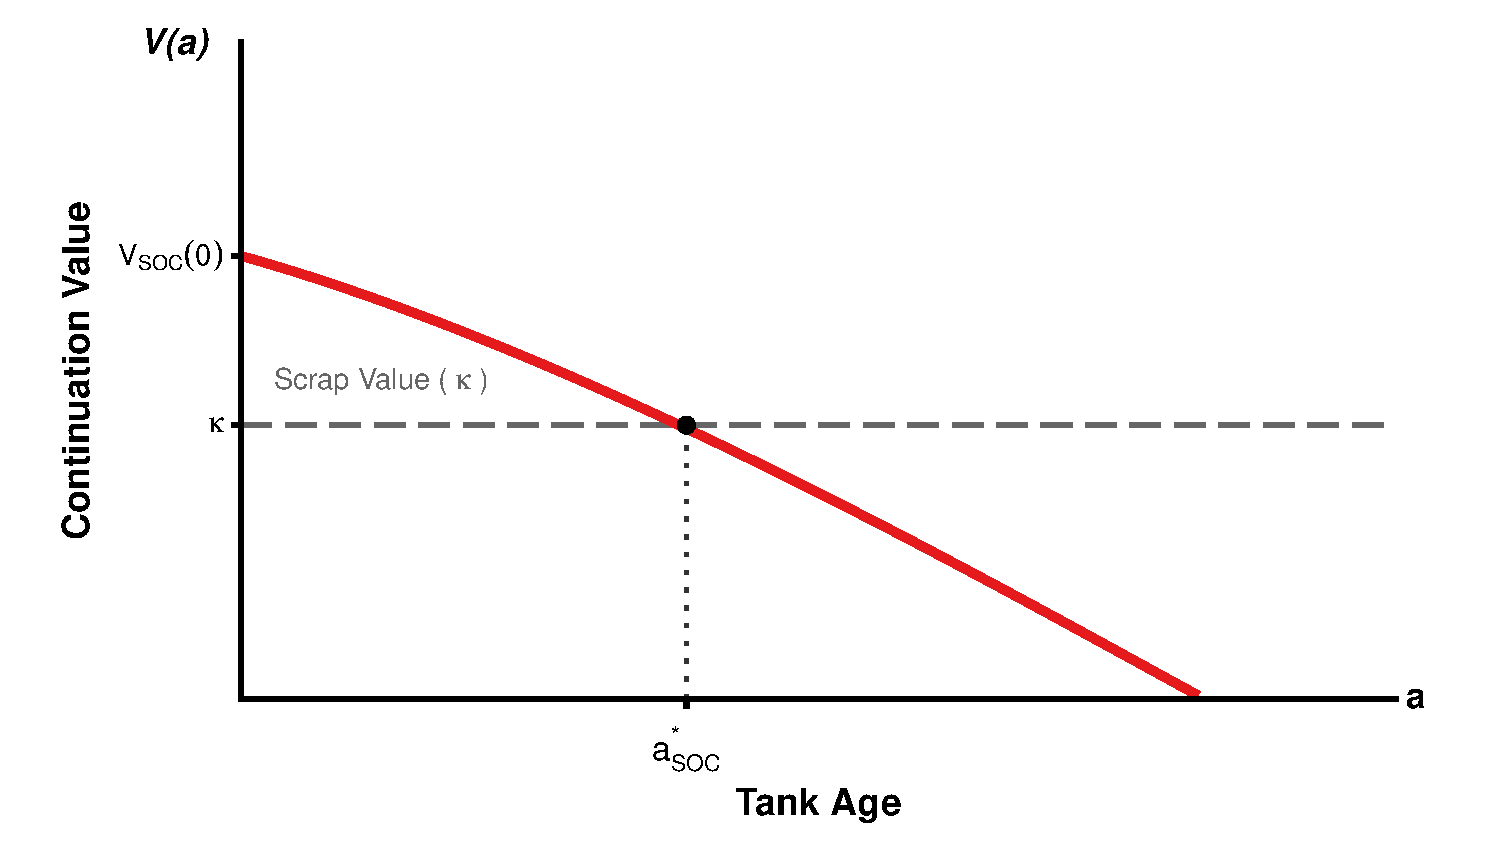
\includegraphics[width=0.92\textwidth,height=0.78\textheight,keepaspectratio]{../../Output/Figures/Slide_Fig_2_SOC_Exit.pdf}
\end{center}
\end{frame}

\begin{frame}{Appendix: Risk-Based vs.~Social Optimum (toy model)}
\phantomsection\label{appendix-risk-based-vs.-social-optimum-toy-model}
\BerkeleyLightMode

\hypertarget{toy-rbvssoc}{}

\vspace{0.2cm}
\begin{center}
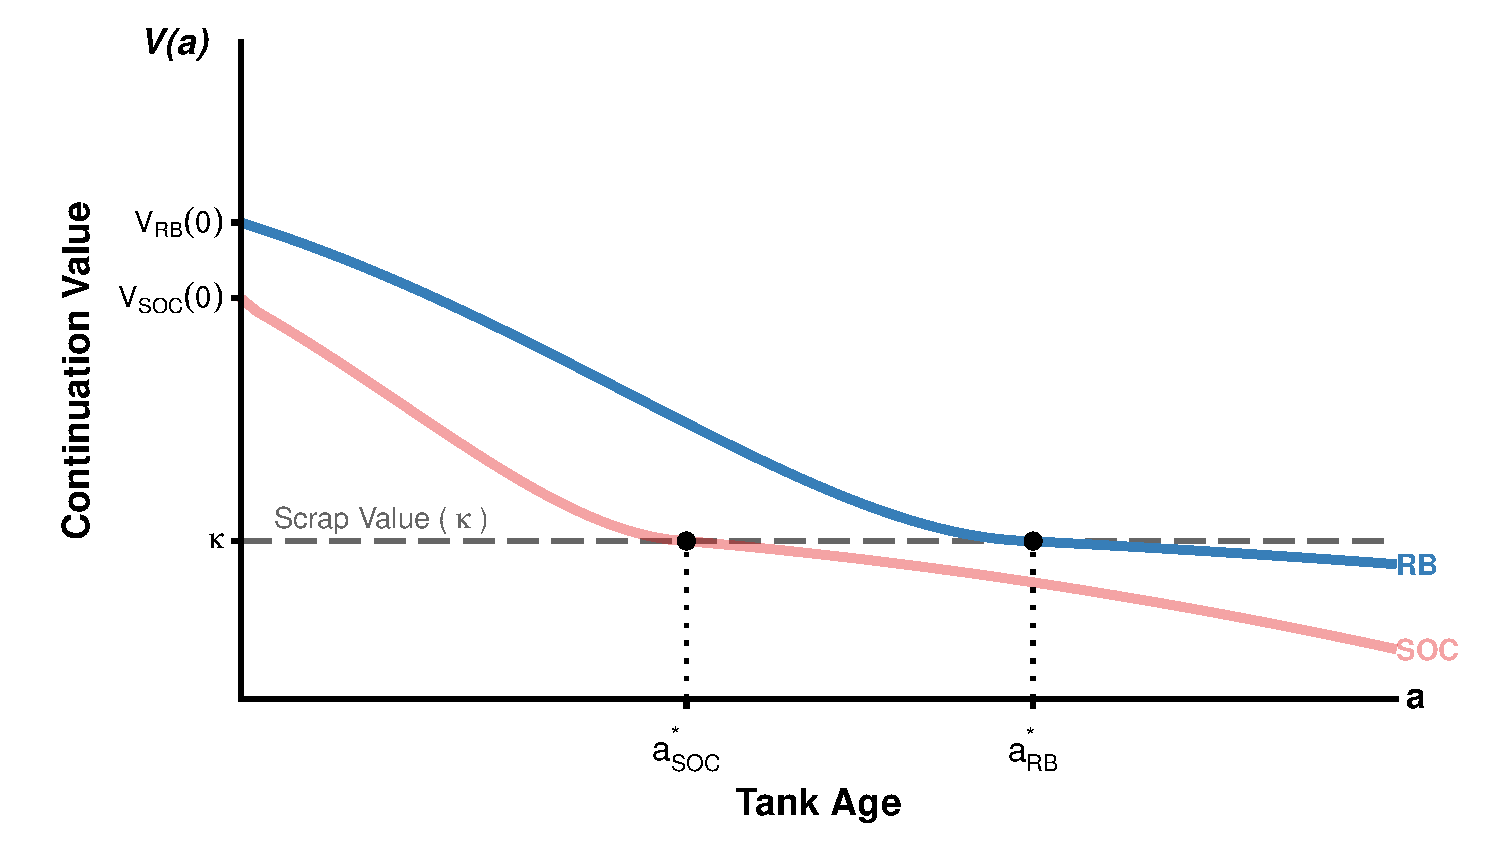
\includegraphics[width=0.92\textwidth,height=0.78\textheight,keepaspectratio]{../../Output/Figures/Slide_Fig_3_SOC_RB_Comparison.pdf}
\end{center}
\end{frame}

\begin{frame}{Appendix: Uniform Premium vs.~Social Optimum (toy model)}
\phantomsection\label{appendix-uniform-premium-vs.-social-optimum-toy-model}
\BerkeleyLightMode

\hypertarget{toy-ffvssoc}{}

\vspace{0.2cm}
\begin{center}
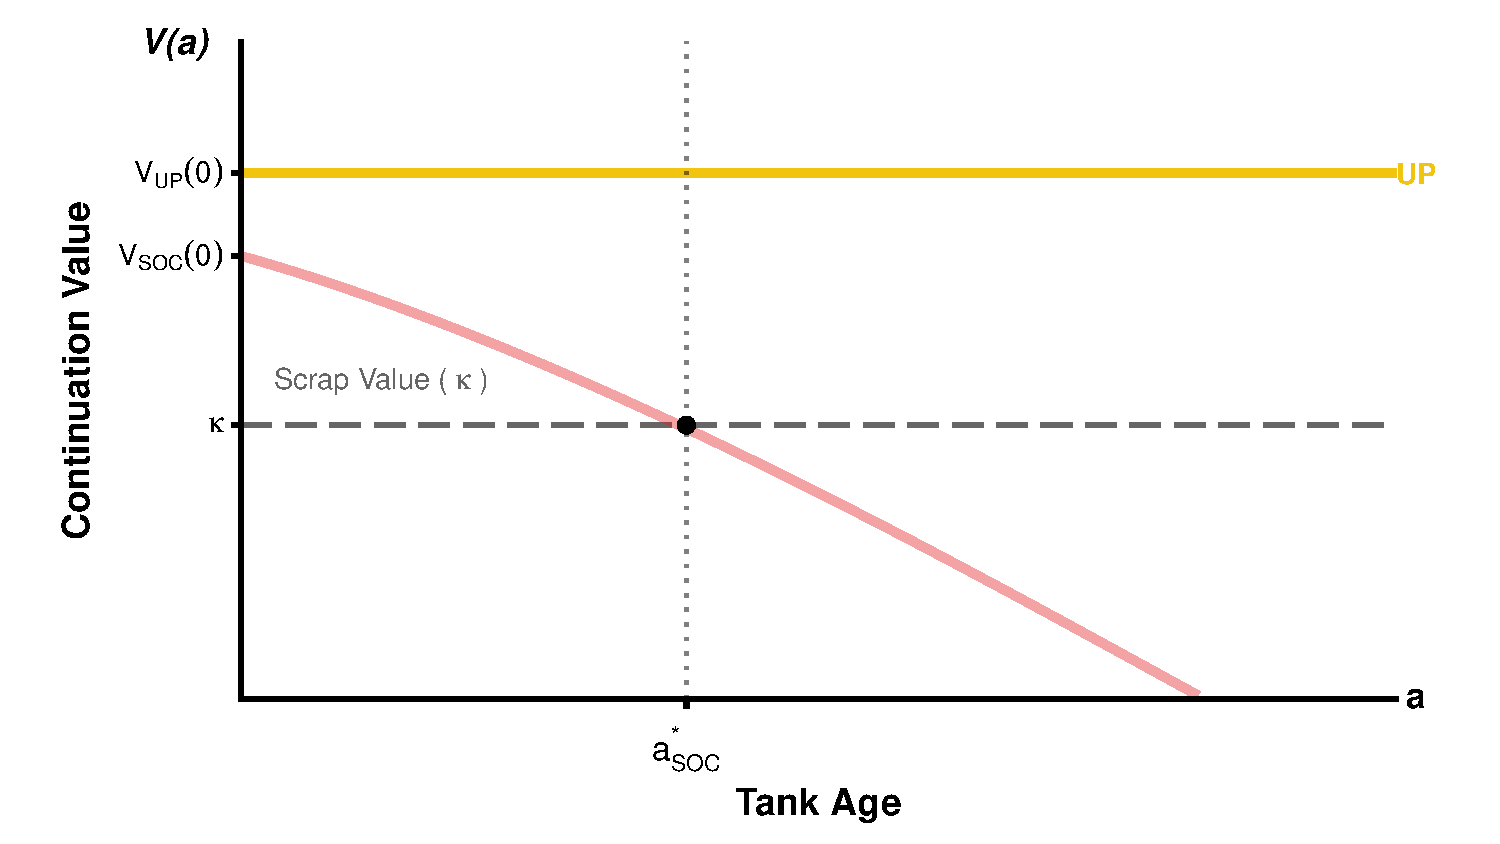
\includegraphics[width=0.92\textwidth,height=0.78\textheight,keepaspectratio]{../../Output/Figures/Slide_Fig_5_SOC_FF_Comparison.pdf}
\end{center}
\end{frame}

\begin{frame}{Appendix: Deadweight Loss Across Regimes (toy model)}
\phantomsection\label{appendix-deadweight-loss-across-regimes-toy-model}
\BerkeleyLightMode

\hypertarget{toy-dwl}{}

\vspace{0.2cm}
\begin{center}
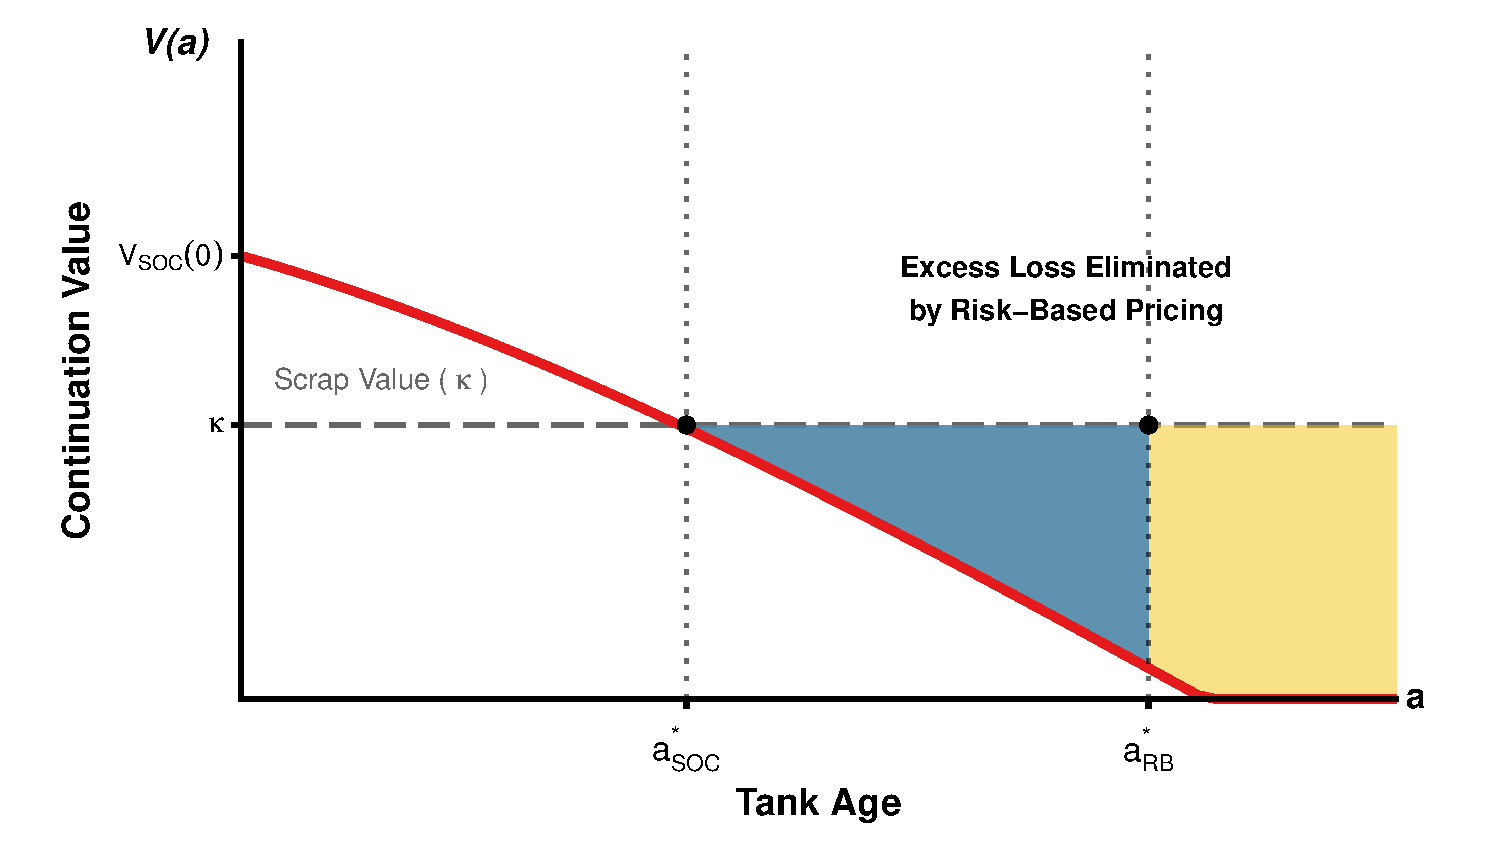
\includegraphics[width=0.92\textwidth,height=0.78\textheight,keepaspectratio]{../../Output/Figures/Slide_Fig_7_Combined_DWL.pdf}
\end{center}
\end{frame}

\begin{frame}{Appendix: FR Compliance: TX is a Private-Insurance Market}
\phantomsection\label{appendix-fr-compliance-tx-is-a-private-insurance-market}
\BerkeleyLightMode

\hypertarget{fr-compliance}{}

\vspace{0.2cm}
\begin{center}
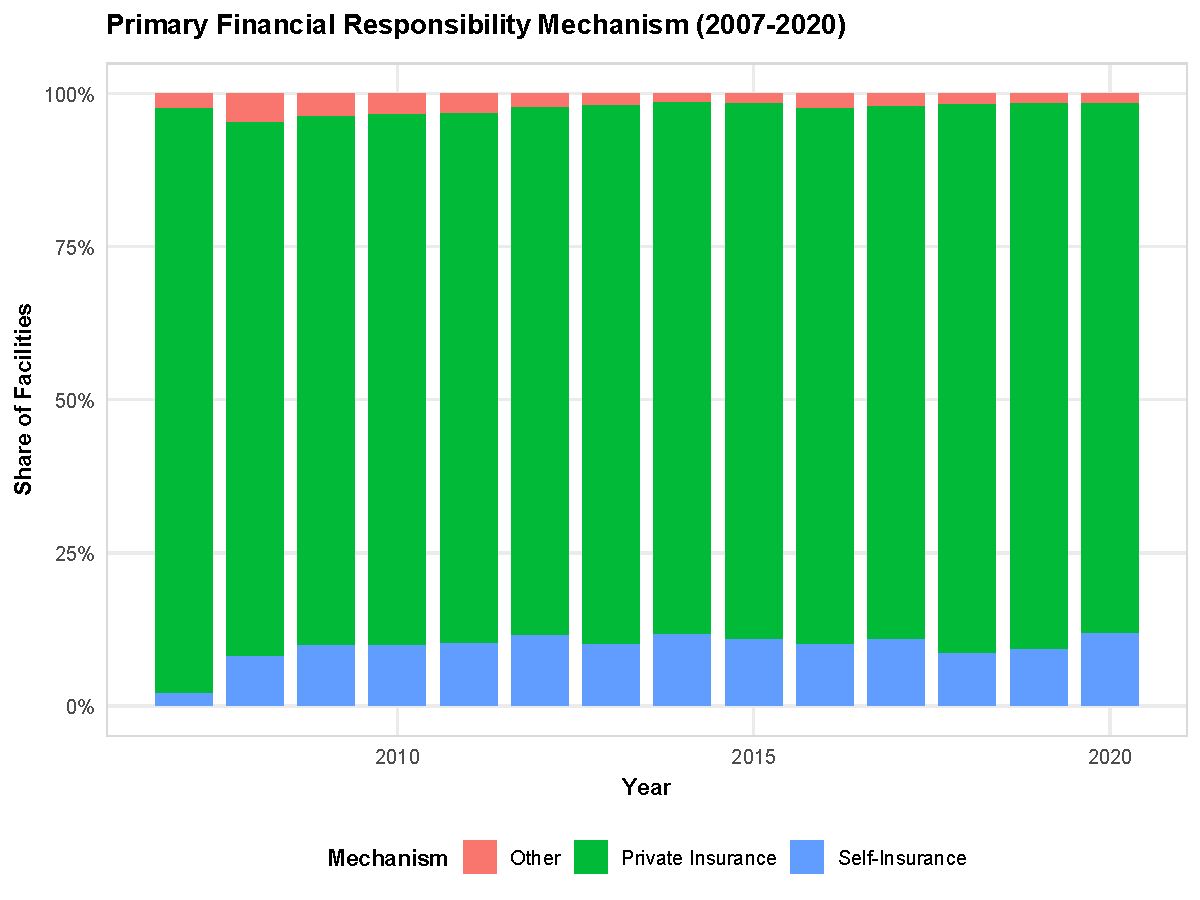
\includegraphics[width=0.92\textwidth,height=0.78\textheight,keepaspectratio]{../../Output/Figures/FigureA_TX_FR_Coverage_Composition.pdf}
\end{center}
\end{frame}

\begin{frame}{Appendix: Market Structure: Concentrated and Stable}
\phantomsection\label{appendix-market-structure-concentrated-and-stable}
\BerkeleyLightMode

\hypertarget{market-hhi}{}

\vspace{0.2cm}
\begin{center}
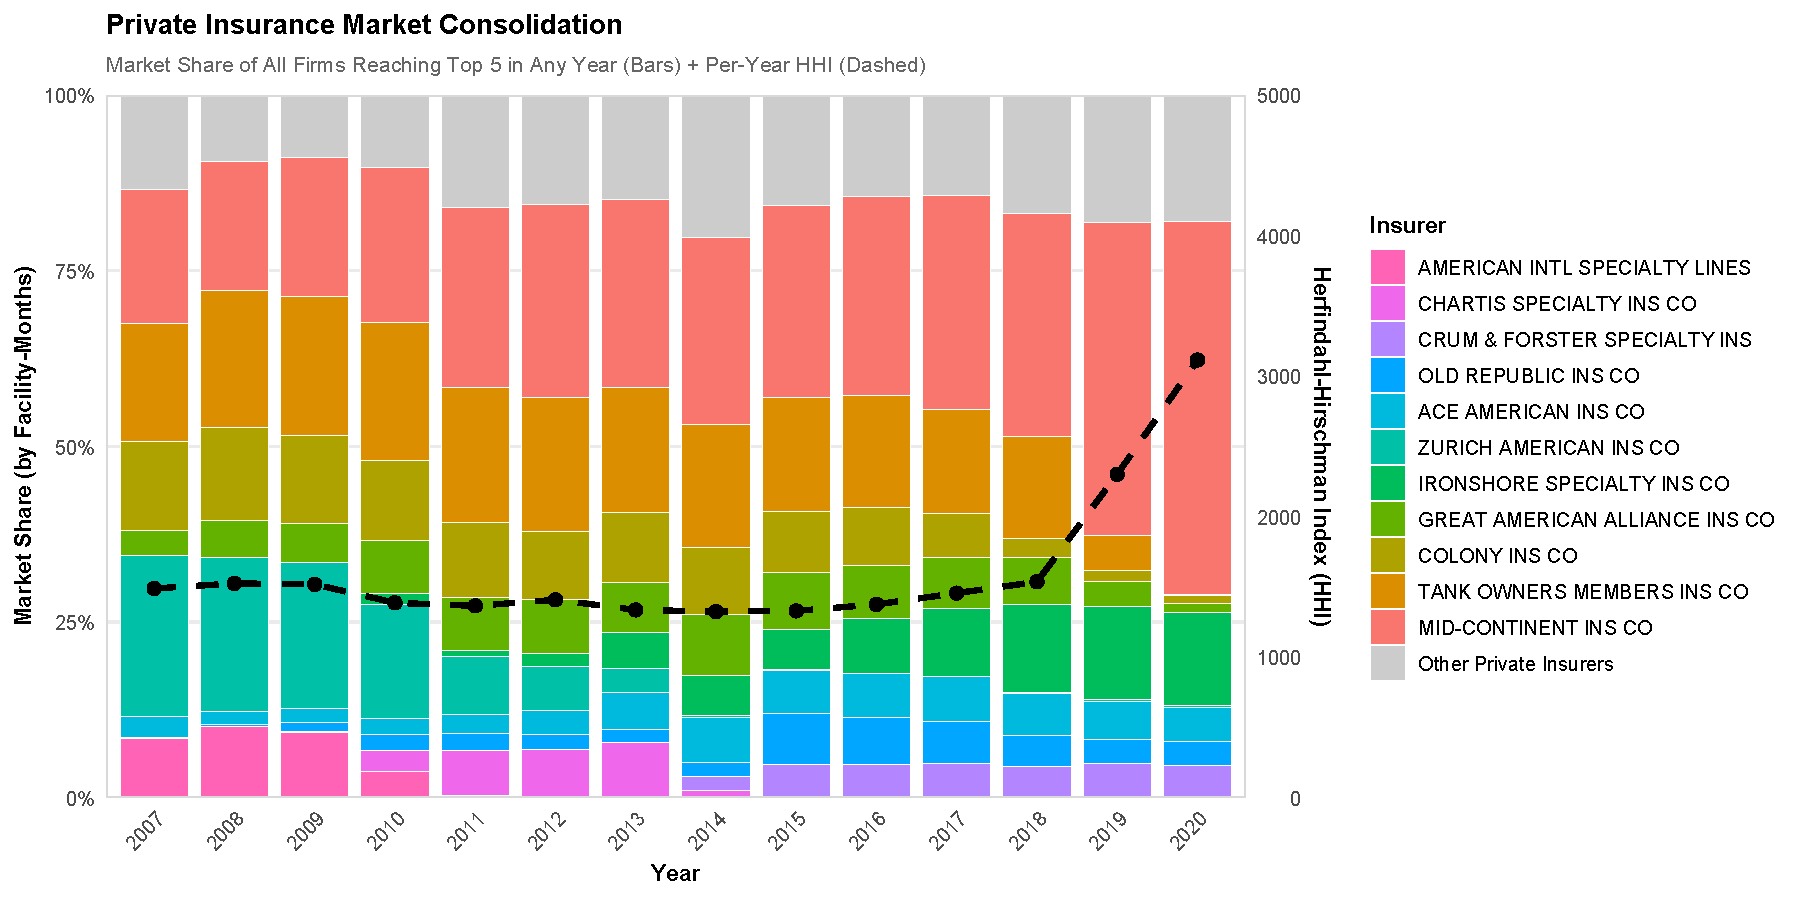
\includegraphics[width=0.92\textwidth,height=0.78\textheight,keepaspectratio]{../../Output/Figures/Figure_TX_FR_Top5_Dominance_HHI.pdf}
\end{center}
\end{frame}

\begin{frame}{Appendix: Cell-Level Goodness of Fit}
\phantomsection\label{appendix-cell-level-goodness-of-fit}
\BerkeleyLightMode

\hypertarget{cell-gof}{}

\vspace{0.2cm}
\begin{center}
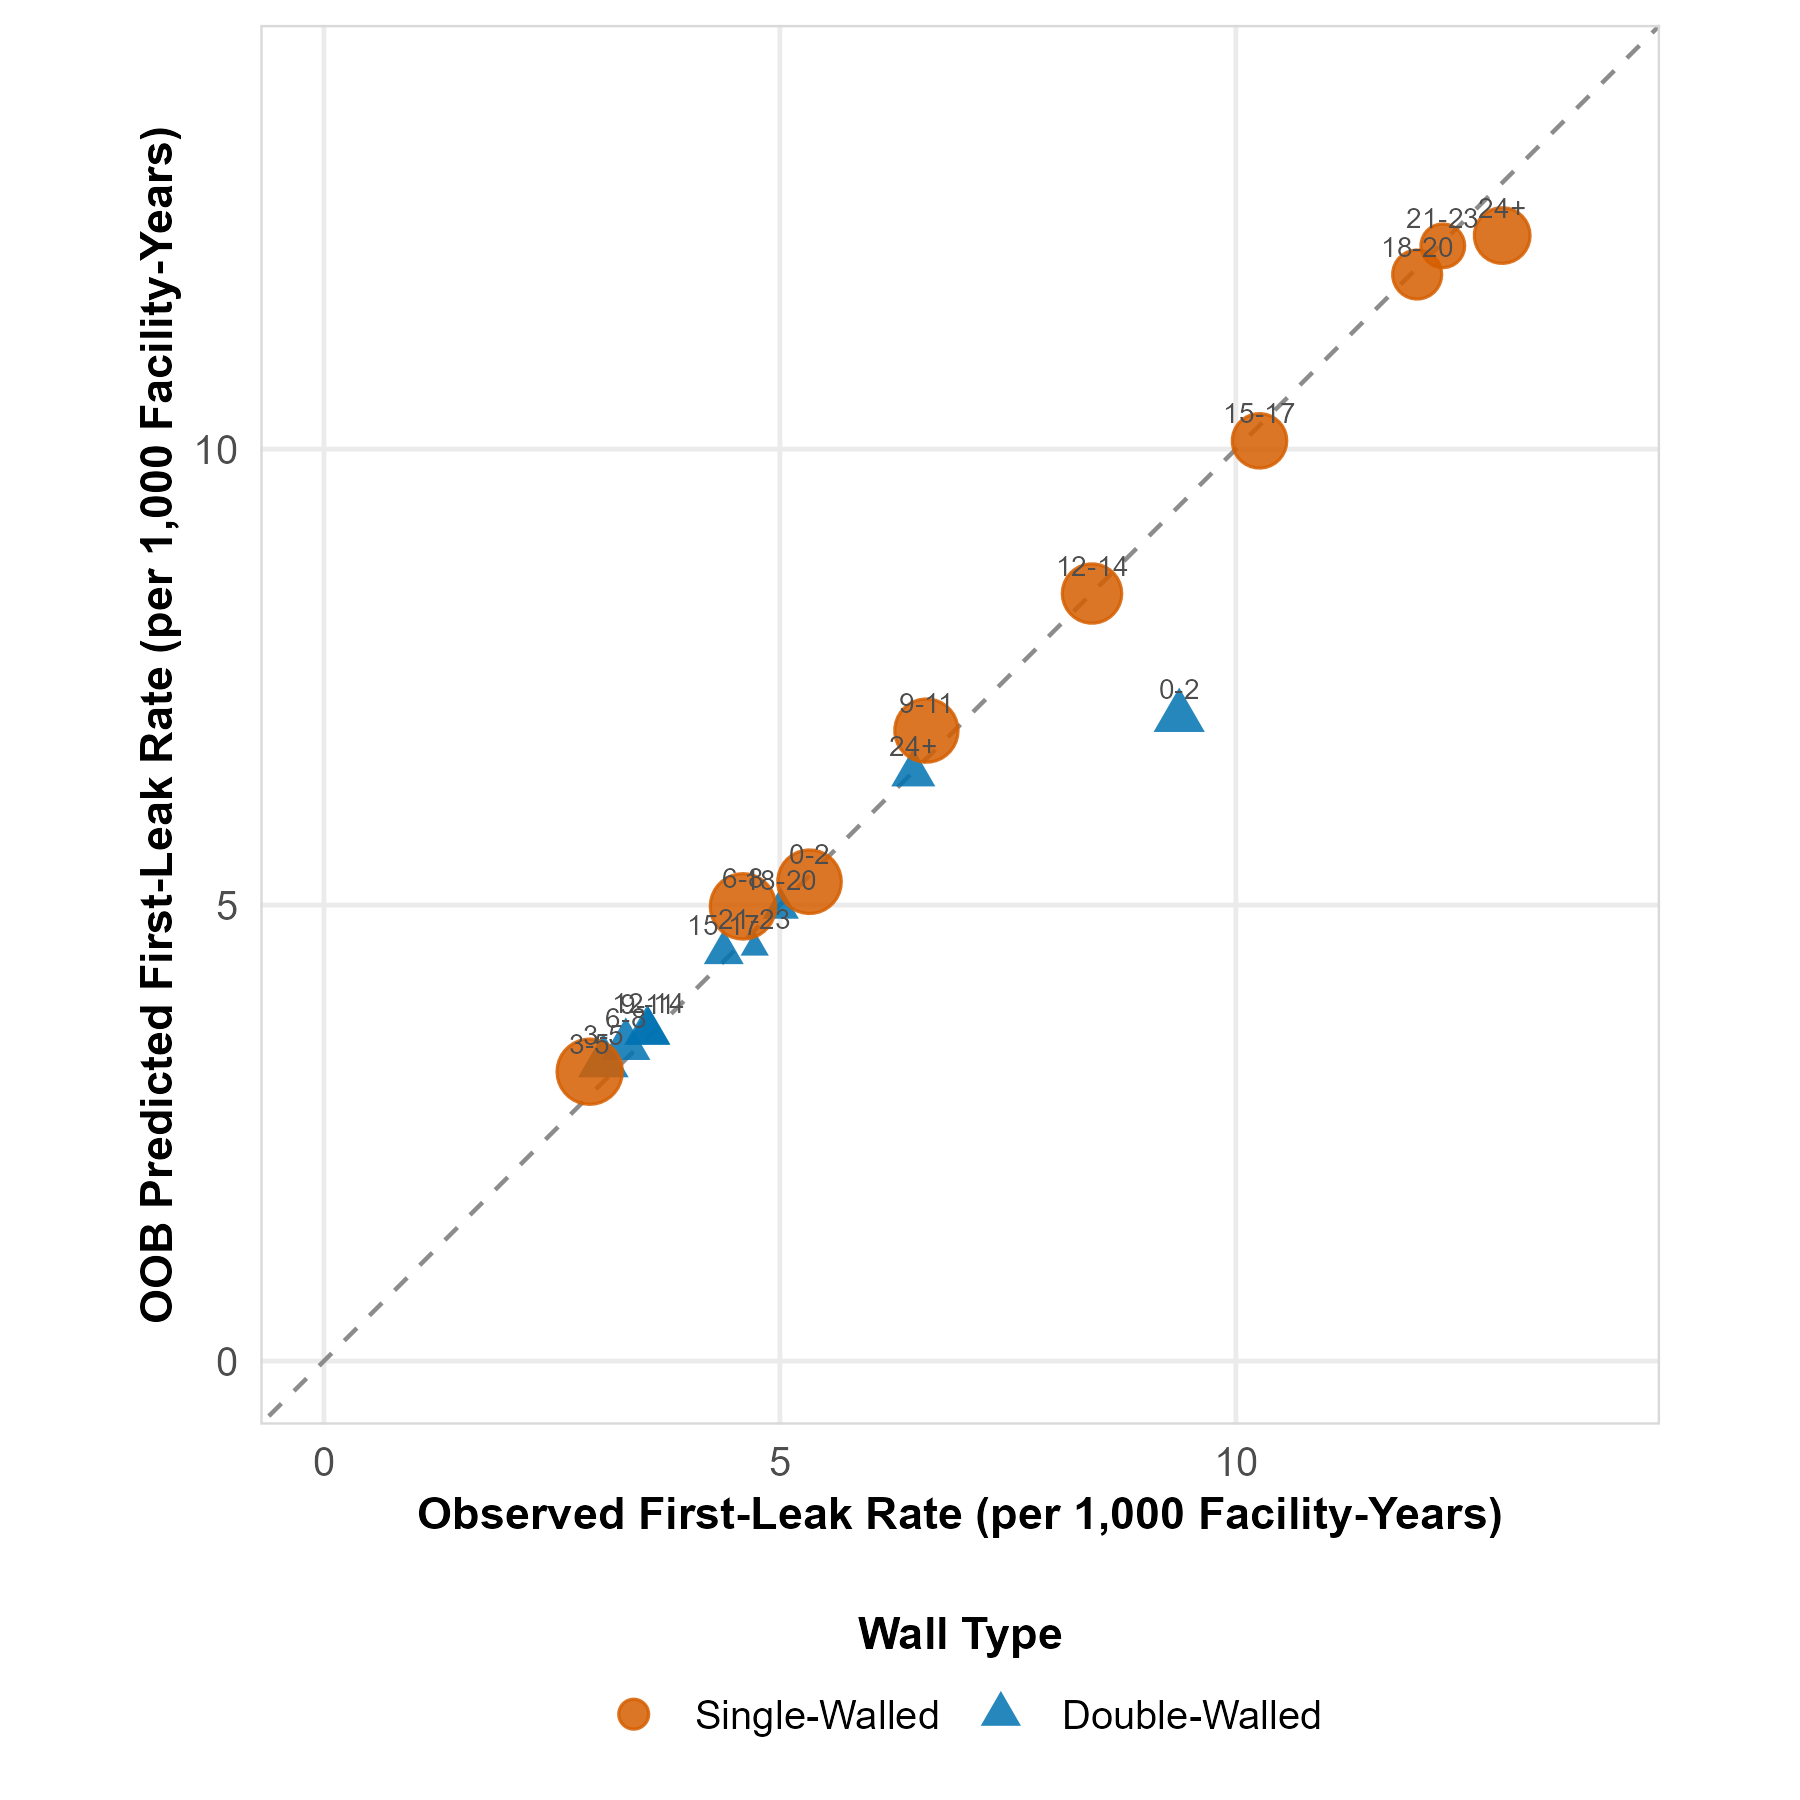
\includegraphics[width=0.92\textwidth,height=0.78\textheight,keepaspectratio]{../../Output/Figures/Figure_CV_CellRisk_GoF.png}
\end{center}
\end{frame}

\begin{frame}{Appendix: ATT by Installation Vintage}
\phantomsection\label{appendix-att-by-installation-vintage}
\BerkeleyLightMode

\hypertarget{vintage-forest}{}

\vspace{0.2cm}
\begin{center}
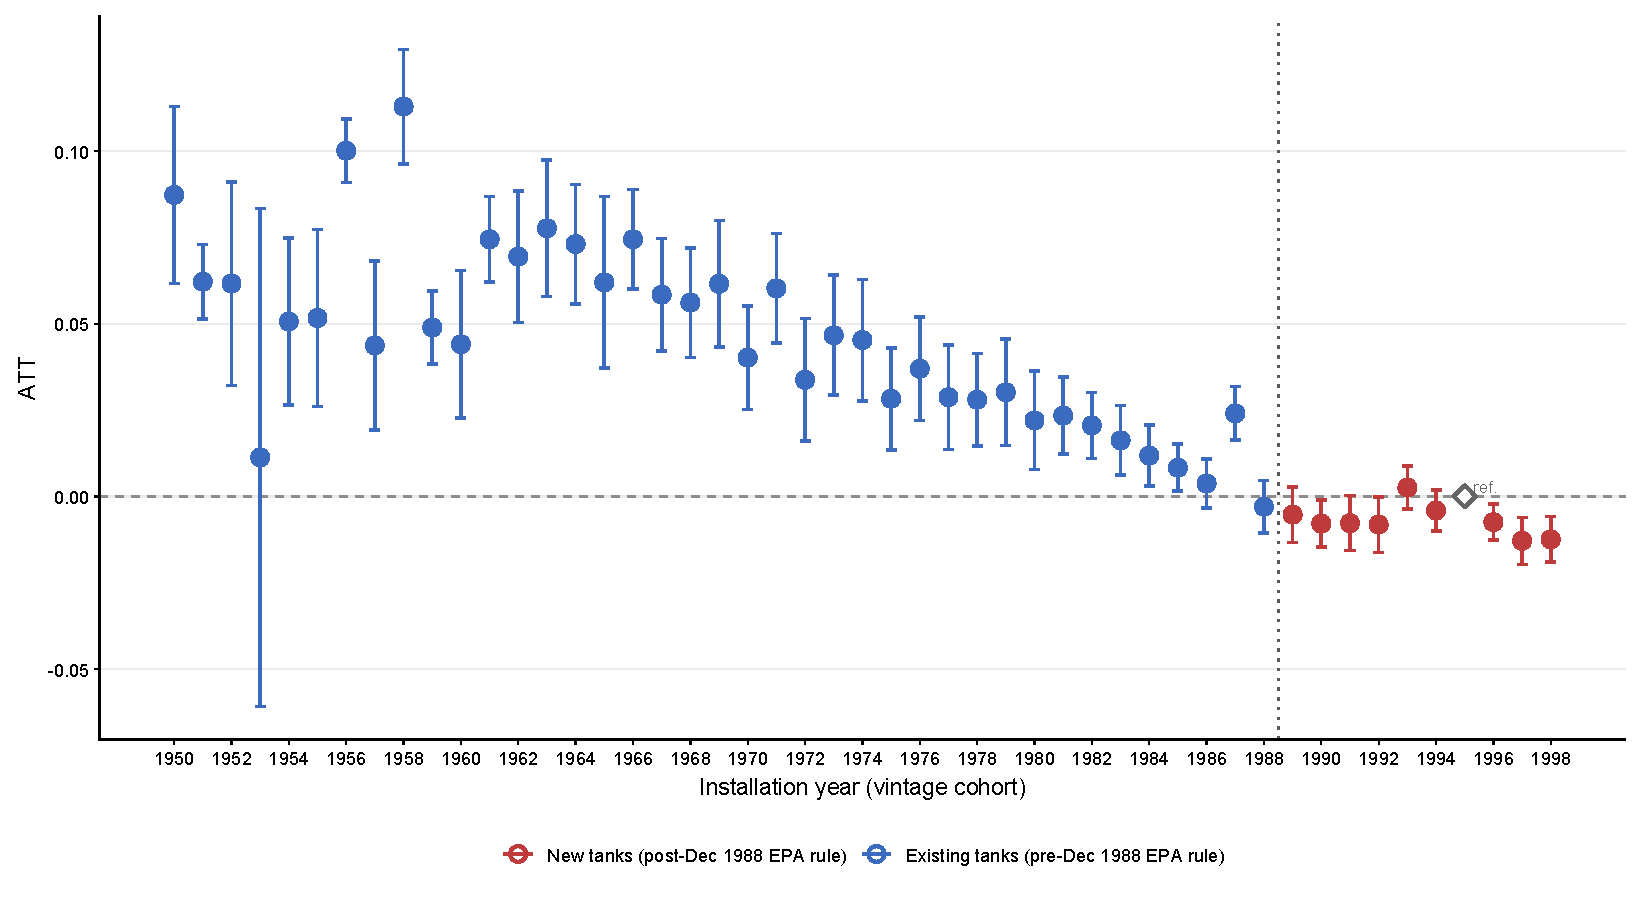
\includegraphics[width=0.92\textwidth,height=0.78\textheight,keepaspectratio]{../../Output/Figures/Fig_Vintage_Forest.pdf}
\end{center}
\end{frame}

\begin{frame}{Appendix: Premium vs.~Per-Tank Expected Loss}
\phantomsection\label{appendix-premium-vs.-per-tank-expected-loss}
\BerkeleyLightMode

\hypertarget{premium-vs-el}{}

\vspace{0.2cm}
\begin{center}
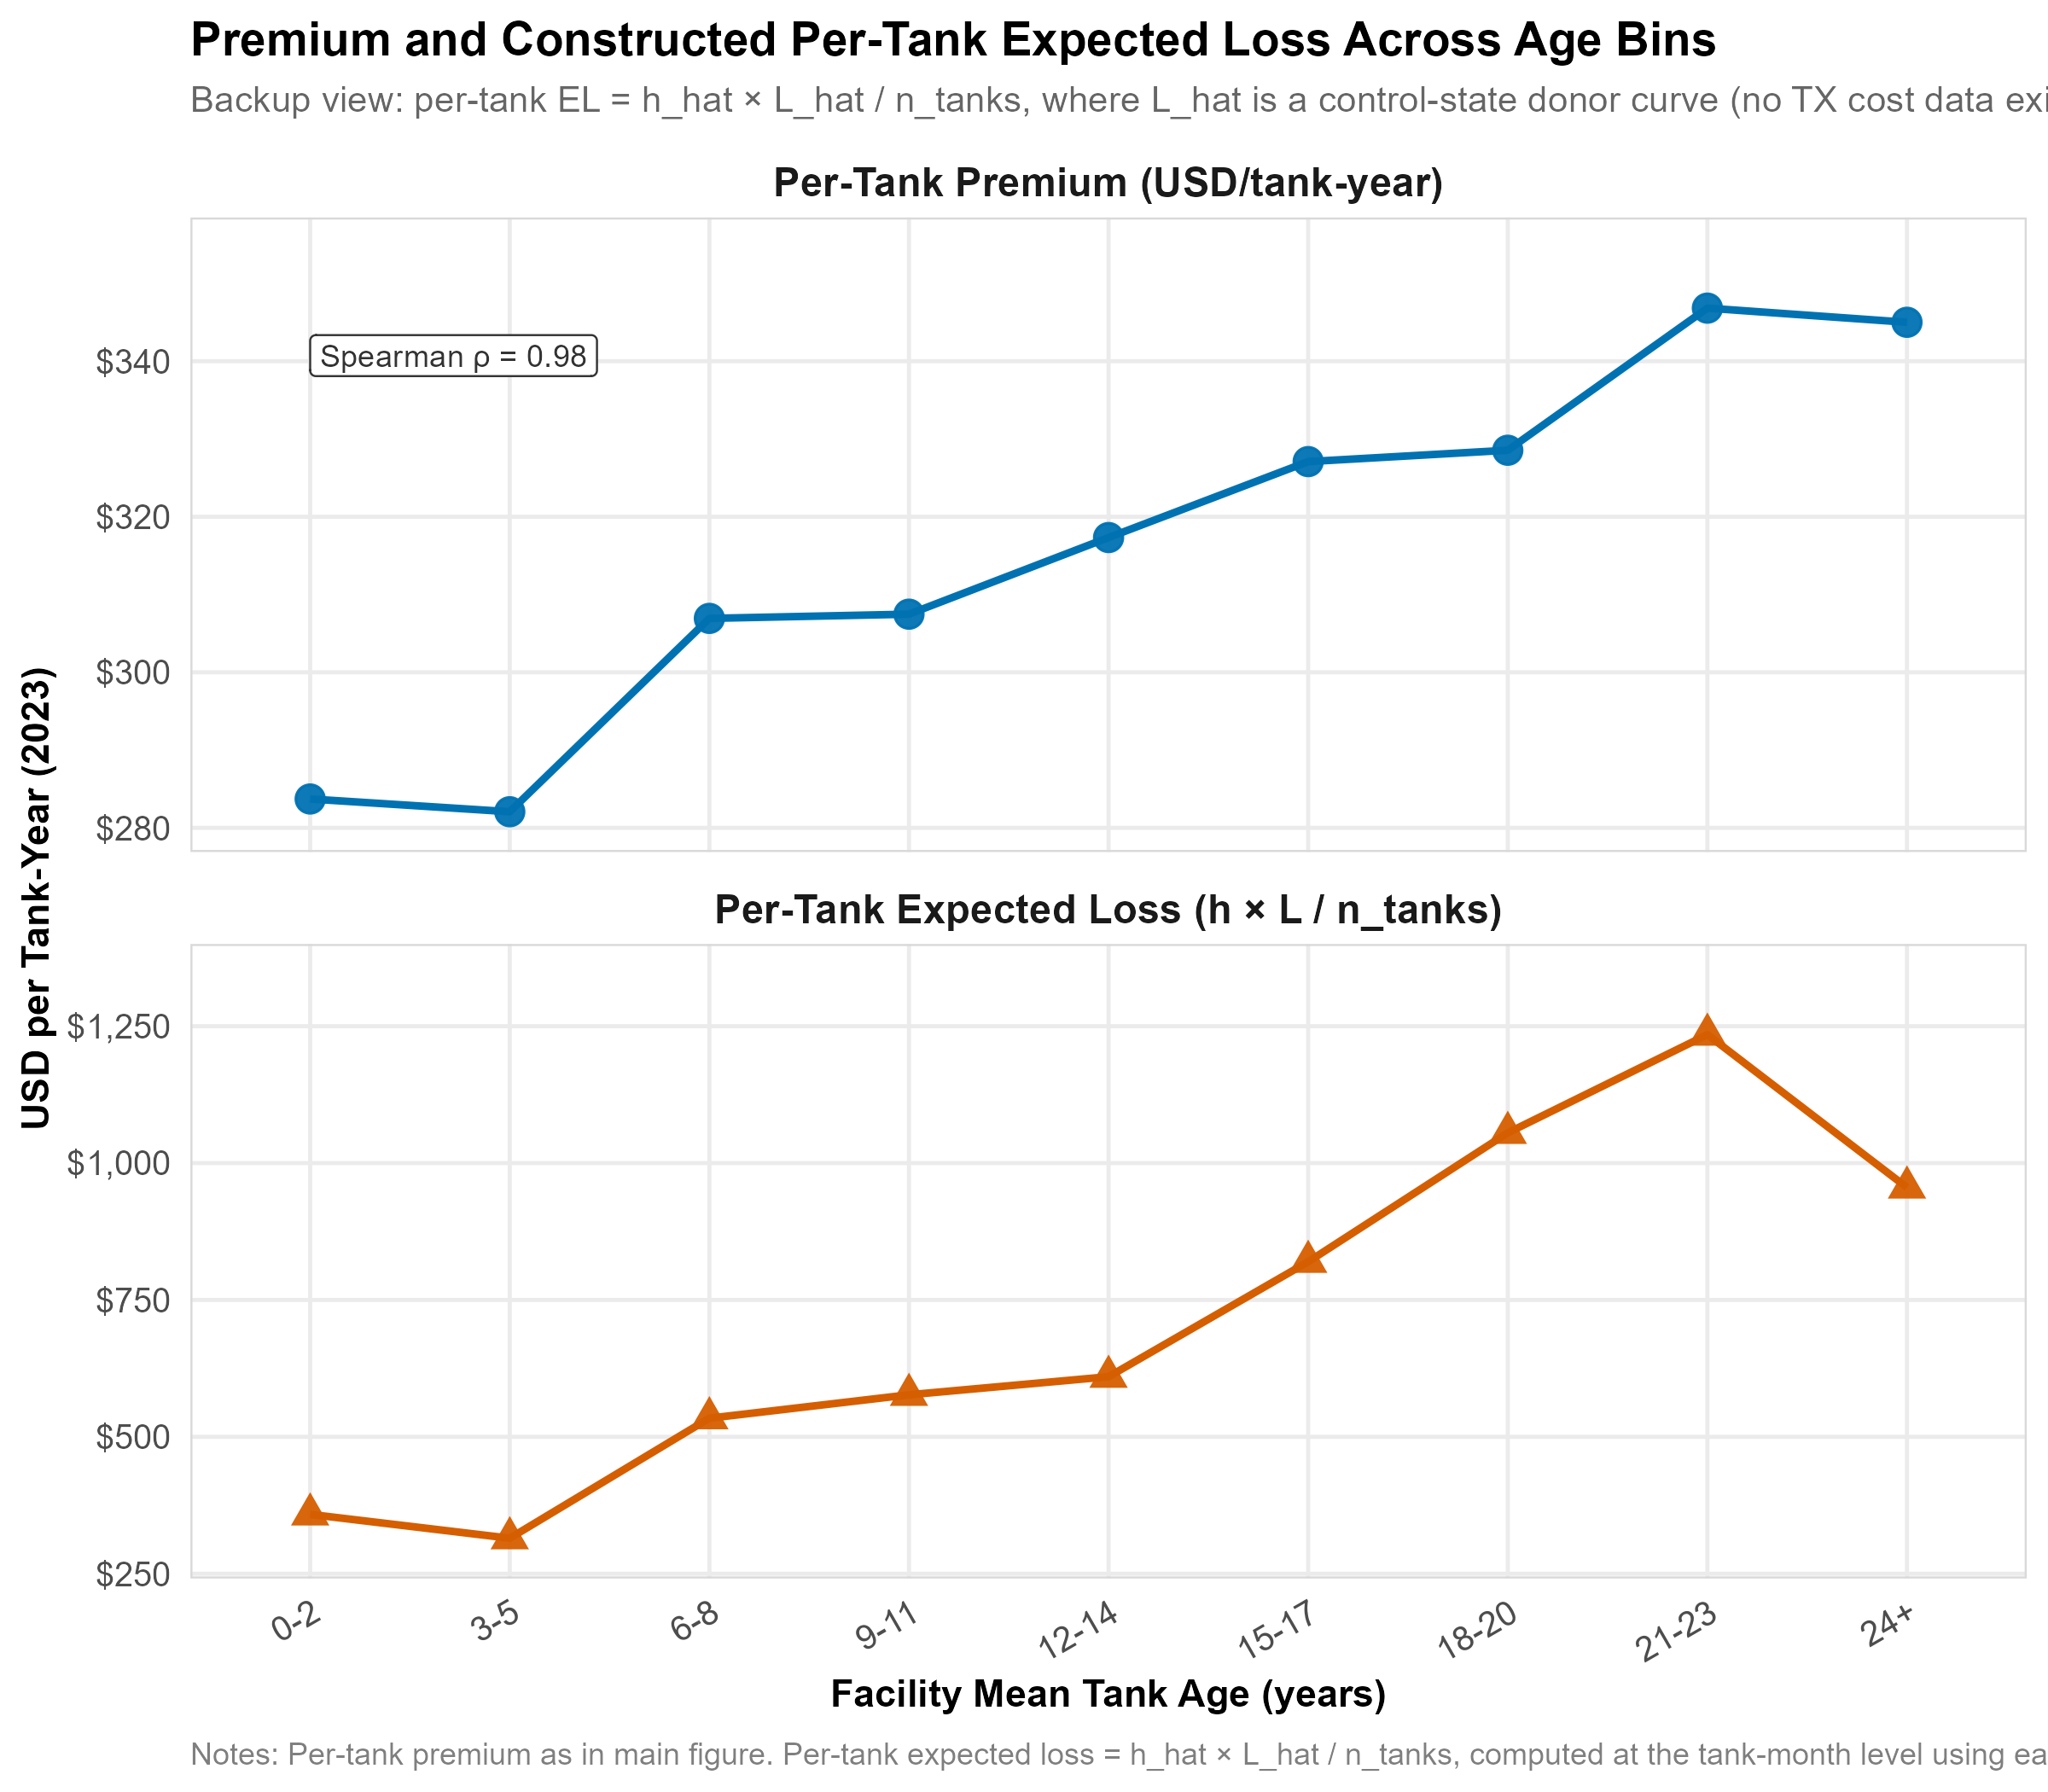
\includegraphics[width=0.92\textwidth,height=0.78\textheight,keepaspectratio]{../../Output/Figures/Figure_Premium_vs_EL_Raw.png}
\end{center}
\end{frame}

\begin{frame}{Appendix: LUST Event Study --- Total Leak Discovery}
\phantomsection\label{appendix-lust-event-study-total-leak-discovery}
\BerkeleyLightMode

\hypertarget{lust-es}{}

\vspace{0.2cm}
\begin{center}
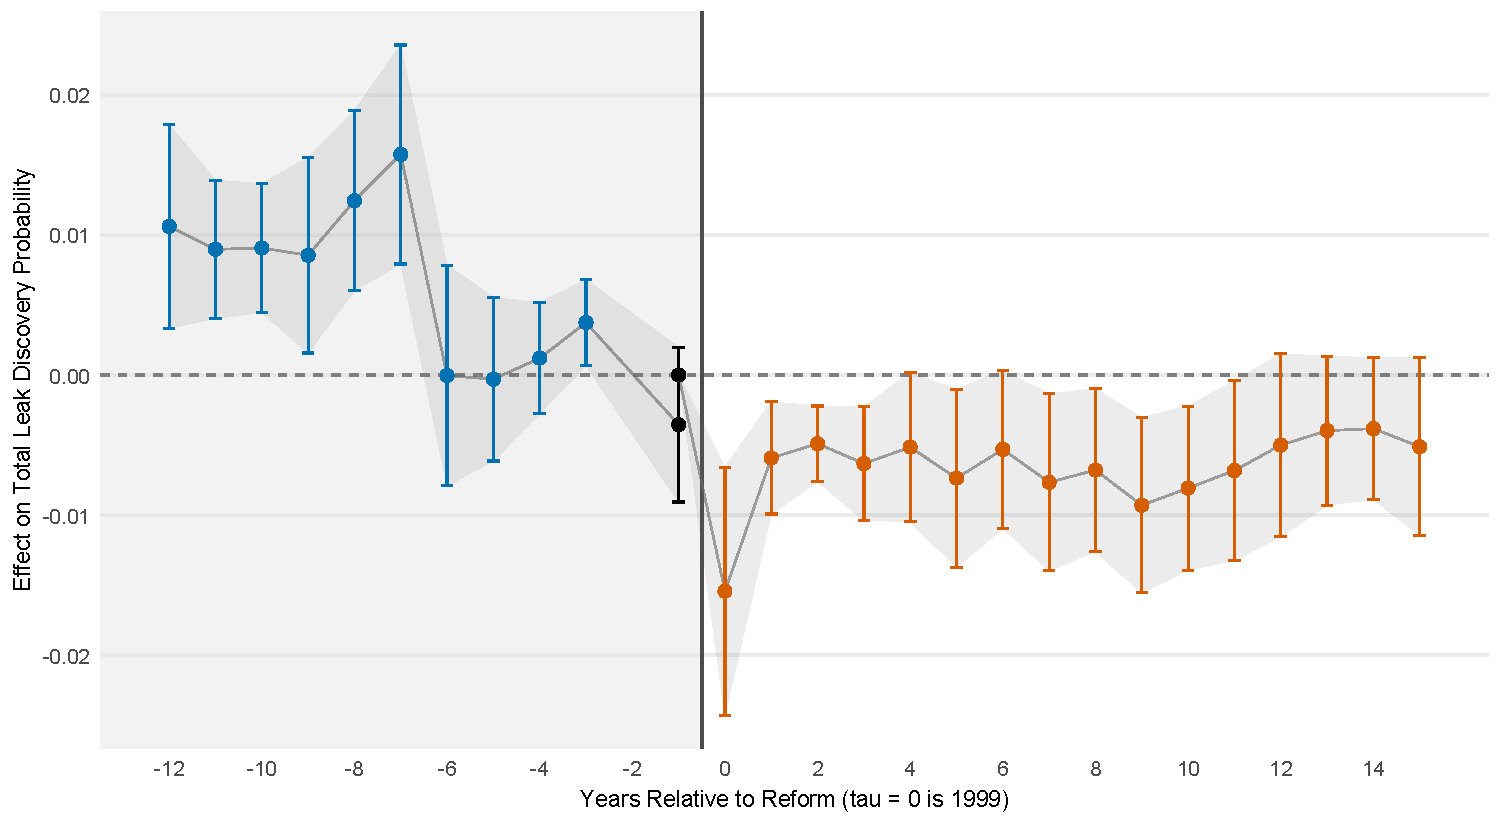
\includegraphics[width=0.92\textwidth,height=0.78\textheight,keepaspectratio]{../../Output/Figures/Figure_ES_LUSTTotal_Appendix.pdf}
\end{center}
\end{frame}

\begin{frame}{Appendix: Subsidy Curve}
\phantomsection\label{appendix-subsidy-curve}
\BerkeleyLightMode

\vspace{0.2cm}
\begin{center}
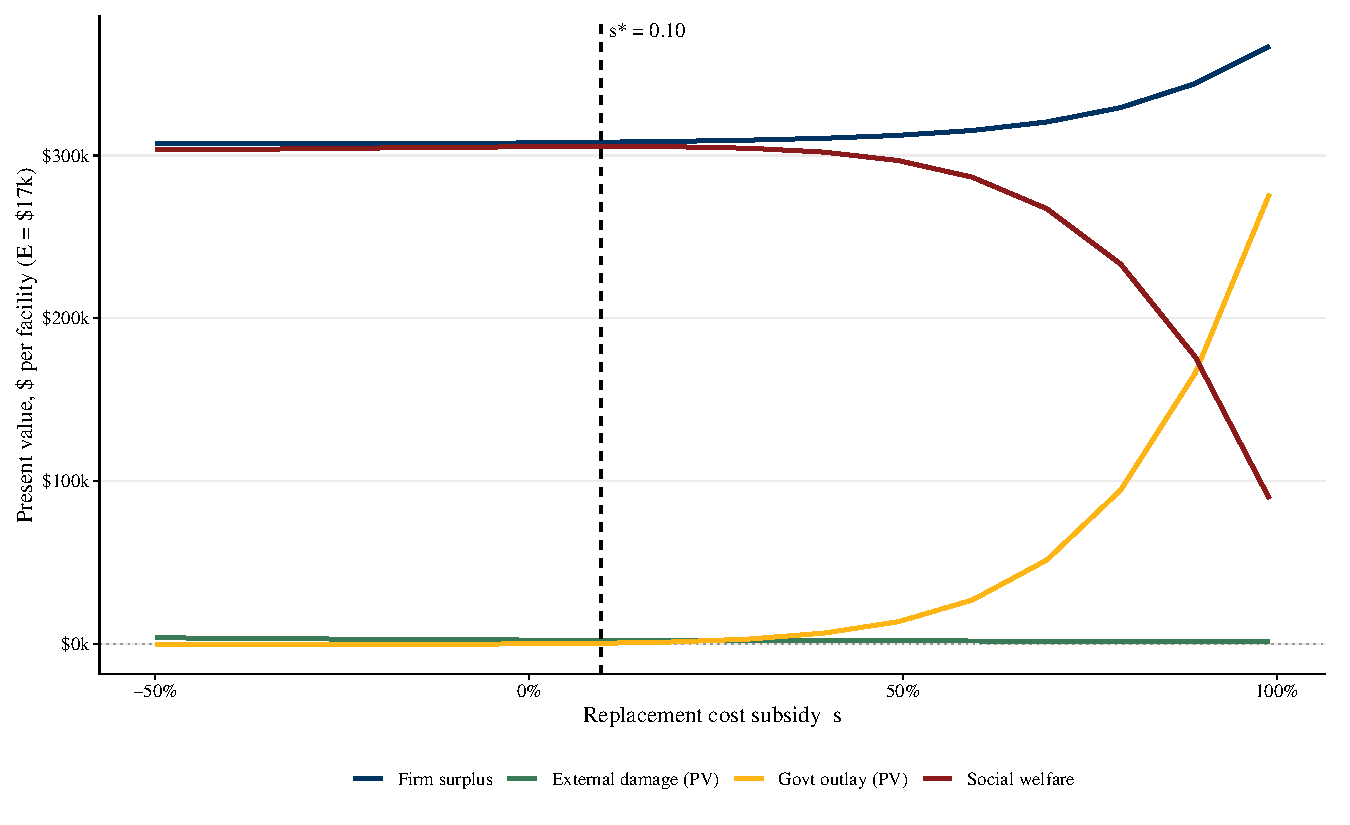
\includegraphics[width=0.92\textwidth,height=0.78\textheight,keepaspectratio]{../../Output/Figures/04j_4p_Subsidy_Curve.pdf}
\end{center}
\end{frame}

\begin{frame}{Appendix: Exit share among closures, by age and wall}
\phantomsection\label{appendix-exit-share-among-closures-by-age-and-wall}
\BerkeleyLightMode

\hypertarget{identif-exit}{}

\vspace{0.1cm}
\begin{center}
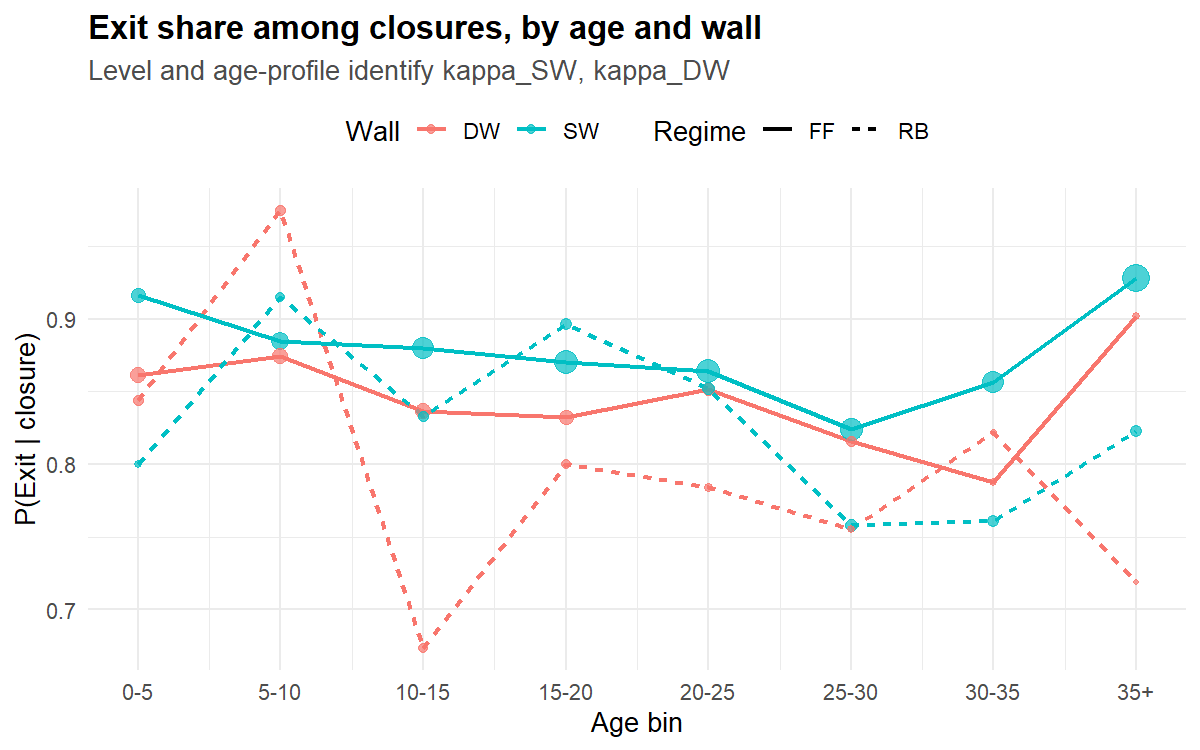
\includegraphics[width=0.9\textwidth,height=0.7\textheight,keepaspectratio]{../../Output/Figures/04q_Identif_ExitShare.png}
\end{center}

\vspace{0.05cm}

\centering\small\textit{The level and age-profile of full exit identify the scrap values $\kappa_{SW}, \kappa_{DW}$.}

\begin{tikzpicture}[remember picture, overlay]
\node[anchor=south west, inner sep=0pt] at ([xshift=10pt, yshift=10pt]current page.south west) {%
  \navbutton[identif-main][fill=BerkeleyBlue, font=\tiny, inner sep=2pt]{$\leftarrow$ back}%
};
\end{tikzpicture}
\end{frame}

\begin{frame}{Appendix: Conditional replace share among closures}
\phantomsection\label{appendix-conditional-replace-share-among-closures}
\BerkeleyLightMode

\hypertarget{identif-replace}{}

\vspace{0.1cm}
\begin{center}
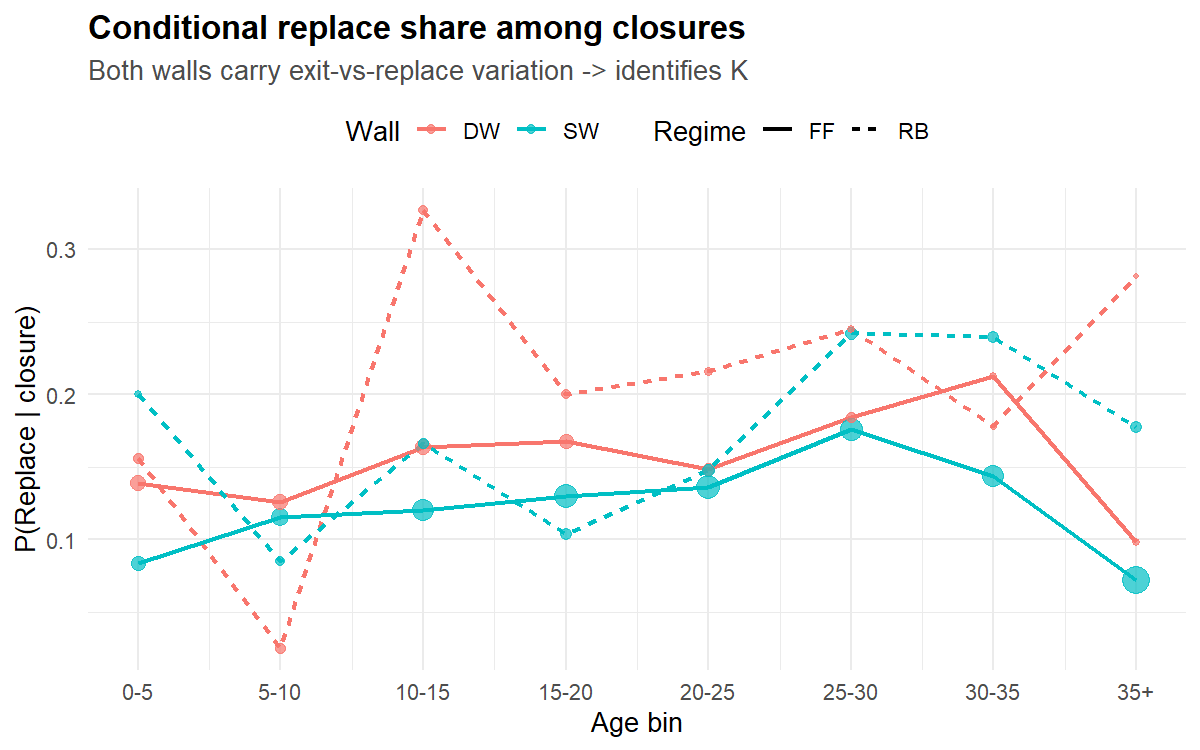
\includegraphics[width=0.9\textwidth,height=0.7\textheight,keepaspectratio]{../../Output/Figures/04q_Identif_ReplaceShare.png}
\end{center}

\vspace{0.05cm}

\centering\small\textit{Both wall types show genuine exit-vs-replace variation, which identifies $K_{SW}$ and $K_{DW}$.}

\begin{tikzpicture}[remember picture, overlay]
\node[anchor=south west, inner sep=0pt] at ([xshift=10pt, yshift=10pt]current page.south west) {%
  \navbutton[identif-main][fill=BerkeleyBlue, font=\tiny, inner sep=2pt]{$\leftarrow$ back}%
};
\end{tikzpicture}
\end{frame}

\begin{frame}{Appendix: Model fit --- SW panel}
\phantomsection\label{appendix-model-fit-sw-panel}
\BerkeleyLightMode

\hypertarget{fit-sw}{}

\vspace{0.1cm}
\begin{center}
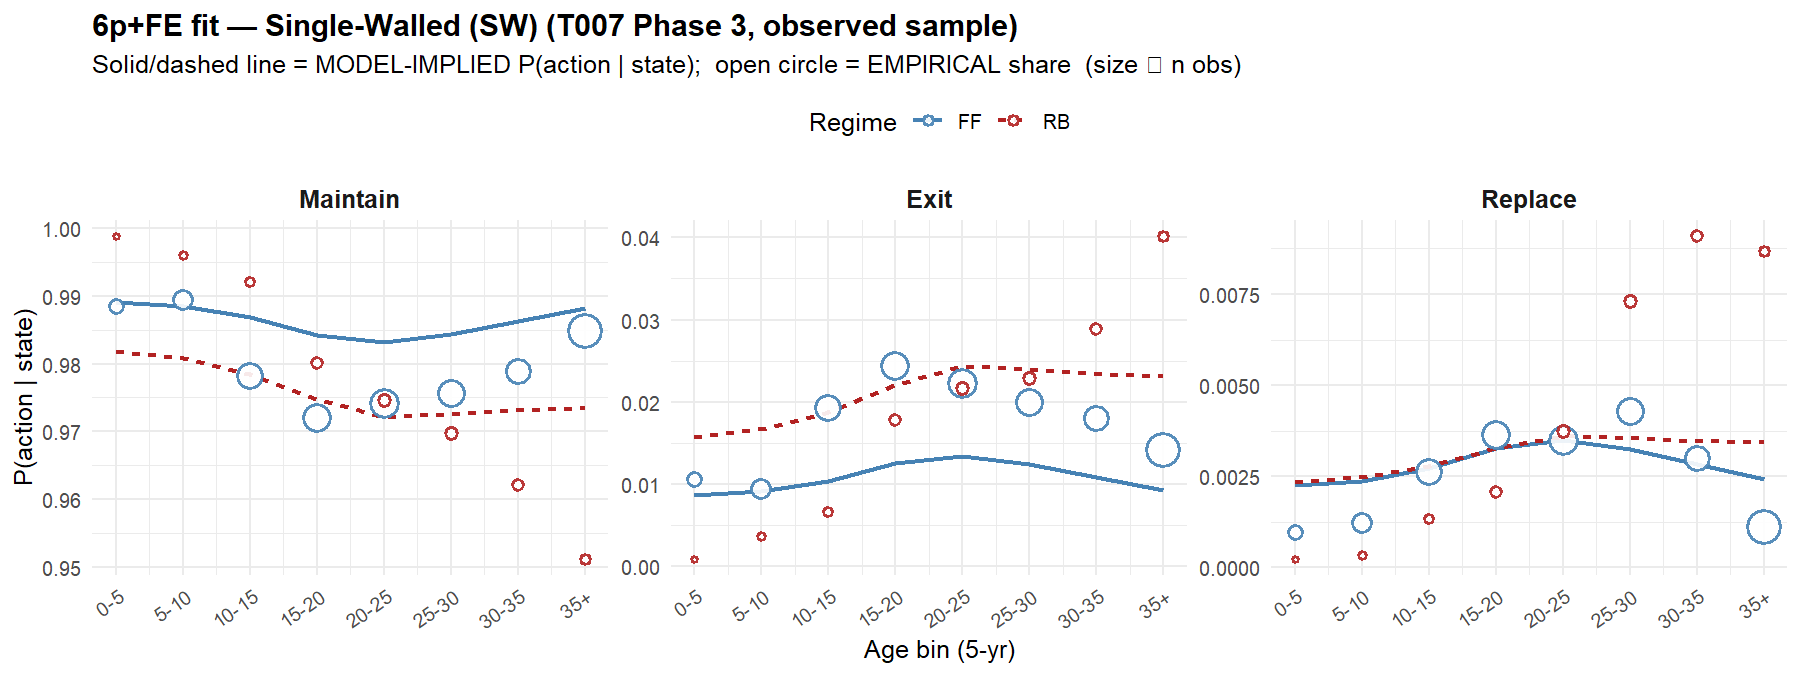
\includegraphics[width=0.92\textwidth,height=0.74\textheight,keepaspectratio]{../../Output/Figures/04o_Fit_6p_SW.png}
\end{center}

\vspace{0.05cm}

\centering\small\textit{Solid lines: model-implied CCPs; open circles: empirical cell shares. 32 cells fit simultaneously across three actions; SW panel.}

\begin{tikzpicture}[remember picture, overlay]
\node[anchor=south west, inner sep=0pt] at ([xshift=10pt, yshift=10pt]current page.south west) {%
  \navbutton[fit-dw][fill=BerkeleyBlue, font=\tiny, inner sep=2pt]{DW fit $\rightarrow$}%
  \hspace{4pt}%
  \navbutton[fit-resid][fill=BerkeleyBlue, font=\tiny, inner sep=2pt]{Per-cell residuals $\rightarrow$}%
};
\end{tikzpicture}
\end{frame}

\begin{frame}{Appendix: Model fit --- DW panel}
\phantomsection\label{appendix-model-fit-dw-panel}
\BerkeleyLightMode

\hypertarget{fit-dw}{}

\vspace{0.2cm}
\begin{center}
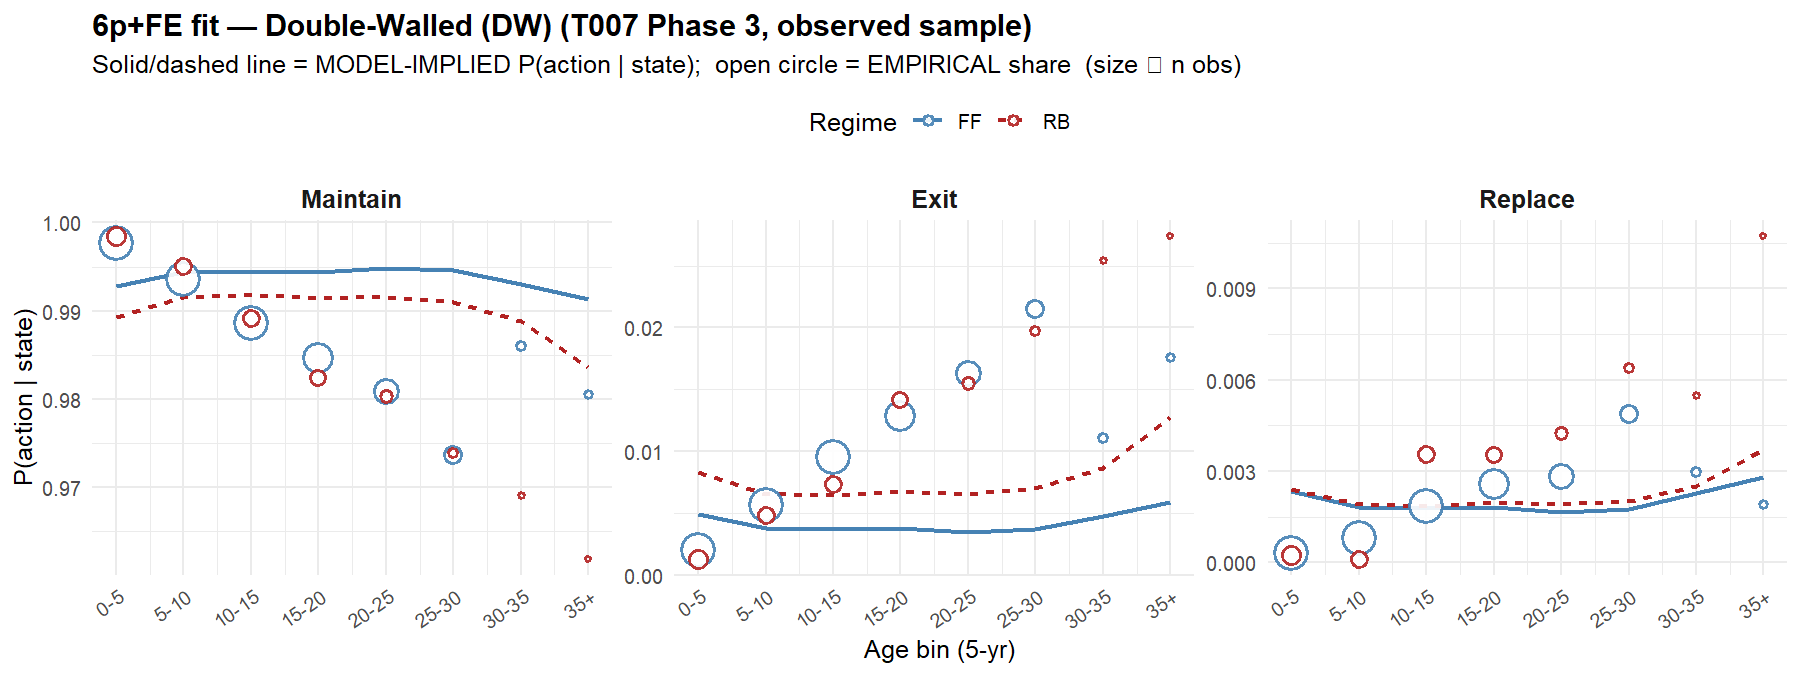
\includegraphics[width=0.92\textwidth,height=0.78\textheight,keepaspectratio]{../../Output/Figures/04o_Fit_6p_DW.png}
\end{center}
\end{frame}

\begin{frame}{Appendix: Per-cell fit residuals (6p)}
\phantomsection\label{appendix-per-cell-fit-residuals-6p}
\BerkeleyLightMode

\hypertarget{fit-resid}{}

\vspace{0.2cm}
\begin{center}
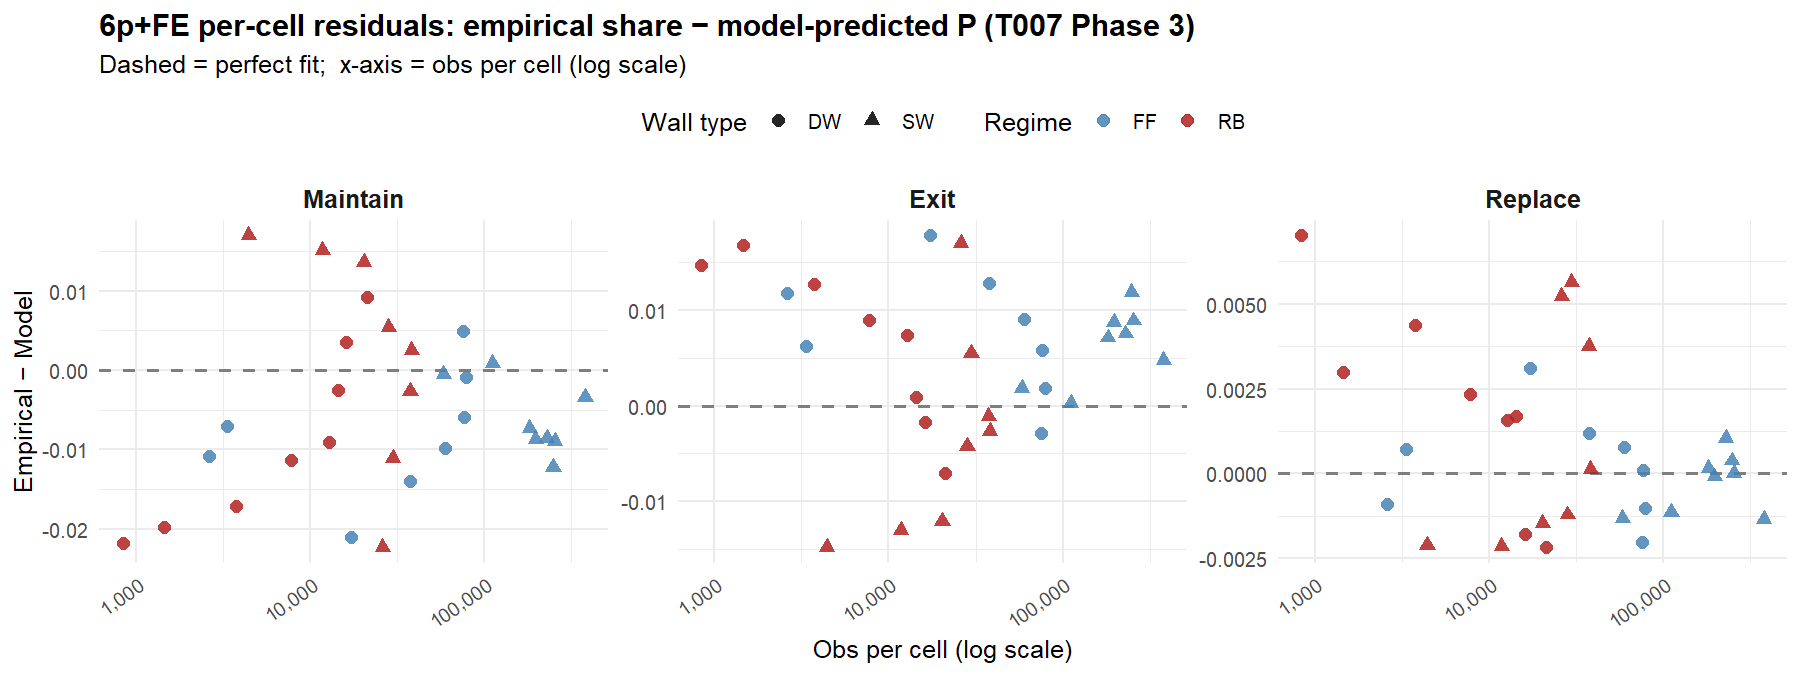
\includegraphics[width=0.92\textwidth,height=0.78\textheight,keepaspectratio]{../../Output/Figures/04o_Fit_6p_AllCells_Residuals.png}
\end{center}
\end{frame}

\begin{frame}{Appendix: Facility size at reform --- Texas vs.~controls}
\phantomsection\label{appendix-facility-size-at-reform-texas-vs.-controls}
\BerkeleyLightMode

\hypertarget{baseline-tanks}{}

\vspace{0.2cm}
\begin{center}
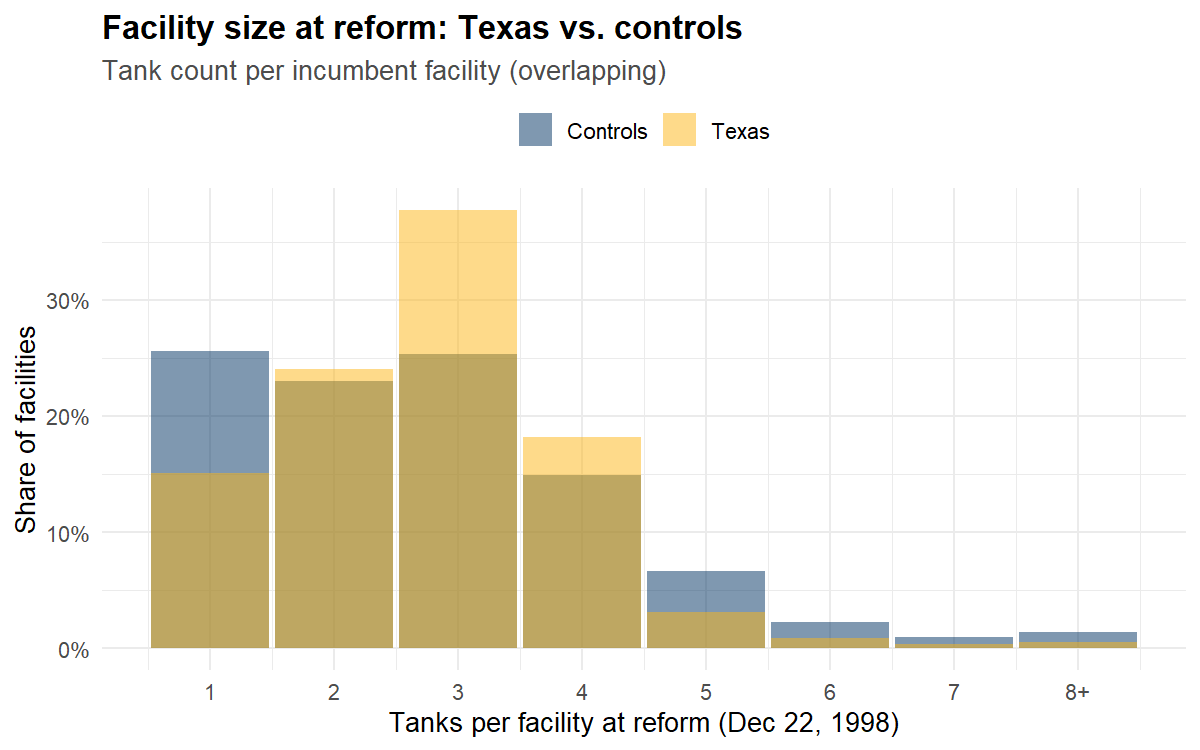
\includegraphics[width=0.72\textwidth,height=0.62\textheight,keepaspectratio]{../../Output/Figures/Fig_Baseline_TanksAtReform.png}
\end{center}

\vspace{0.05cm}

\centering\small\textit{Tank count per incumbent facility on Dec 22, 1998. Texas facilities skew larger (more 3--4 tank facilities); controls have more single-tank facilities.}

\begin{tikzpicture}[remember picture, overlay]
\node[anchor=south west, inner sep=0pt] at ([xshift=10pt, yshift=10pt]current page.south west) {%
  \navbutton[baseline-table][fill=BerkeleyBlue, font=\tiny, inner sep=2pt]{$\leftarrow$ back}%
  \hspace{3pt}%
  \navbutton[baseline-cap][fill=BerkeleyBlue, font=\tiny, inner sep=2pt]{Capacity $\rightarrow$}%
};
\end{tikzpicture}
\end{frame}

\begin{frame}{Appendix: Facility capacity at reform --- Texas
vs.~controls}
\phantomsection\label{appendix-facility-capacity-at-reform-texas-vs.-controls}
\BerkeleyLightMode

\hypertarget{baseline-cap}{}

\vspace{0.2cm}
\begin{center}
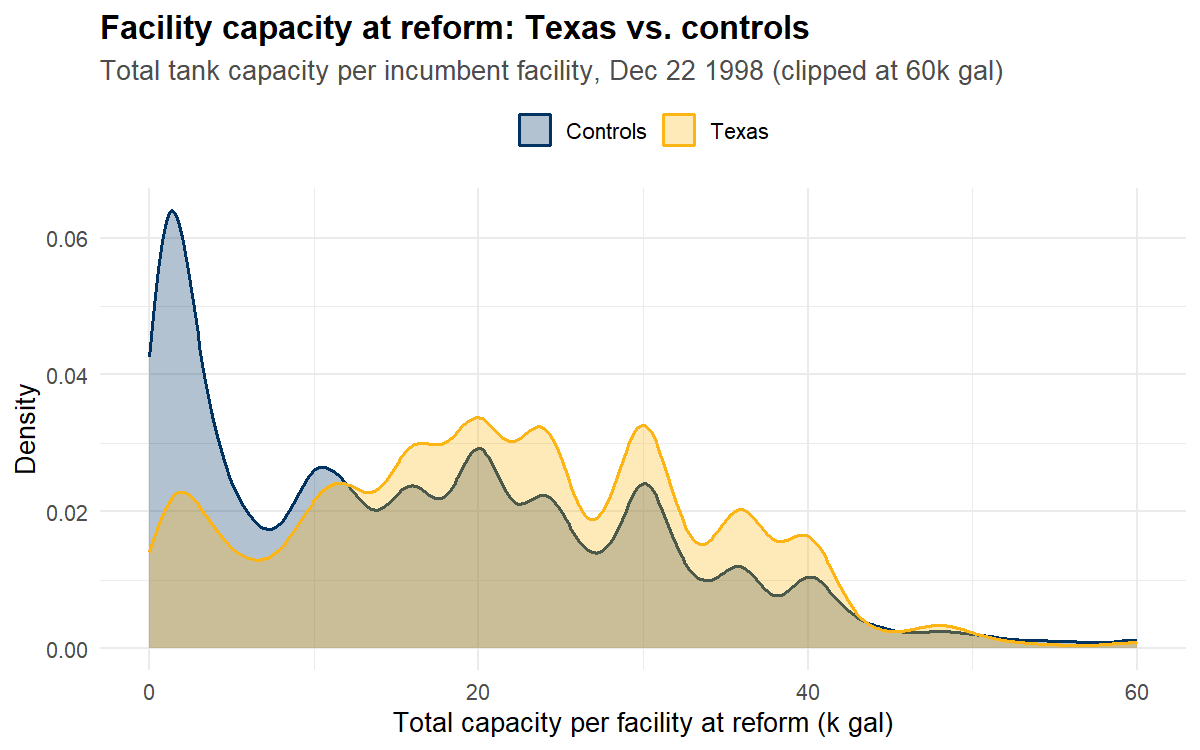
\includegraphics[width=0.72\textwidth,height=0.62\textheight,keepaspectratio]{../../Output/Figures/Fig_Baseline_CapacityAtReform.png}
\end{center}

\vspace{0.05cm}

\centering\small\textit{Total tank capacity per incumbent facility on Dec 22, 1998 (clipped at 60k gal). Controls have a large mass of small single-tank facilities; Texas capacity is shifted right.}

\begin{tikzpicture}[remember picture, overlay]
\node[anchor=south west, inner sep=0pt] at ([xshift=10pt, yshift=10pt]current page.south west) {%
  \navbutton[baseline-table][fill=BerkeleyBlue, font=\tiny, inner sep=2pt]{$\leftarrow$ back}%
};
\end{tikzpicture}
\end{frame}

\begin{frame}{Appendix: What the model captures --- and where it
strains}
\phantomsection\label{appendix-what-the-model-captures-and-where-it-strains}
\BerkeleyLightMode

\hypertarget{portfolio-summary}{}

\small
\textbf{The model.} Single-agent optimal-stopping DDC. Each \emph{facility} $=$ one representative tank on a 32-cell grid (age $\times$ wall $\times$ regime); each year it chooses \textbf{maintain / exit / replace}.
\vspace{0.1cm}
\textbf{Captures well.} The dominant margin --- \textbf{exit} as tanks age, and its response to the premium. Full exits are coded correctly; $\gamma_{\text{price}}$ and $\gamma_{\text{risk}}$ are identified off this well-measured margin.
\vspace{0.1cm}
\textbf{Strains} --- all from one assumption, \emph{a facility is a portfolio, not one tank}:
\begin{itemize}\setlength{\itemsep}{1pt}
\item \textbf{No partial-closure action} --- downsizing (close one tank, keep operating) is coded Maintain. Small overall (0.36\%), concentrated at large facilities.
\item \textbf{Mis-specified ``replace'' transition} --- real upgrades are partial, so 98\% land off the model's reset-to-one-new-tank support.
\item \textbf{Omitted state (facility size)} --- choice probabilities vary by size; the model averages over it.
\end{itemize}

\vfill
\centering\footnotesize\textit{Clean: maintain / exit / premium. Strained: the portfolio (size $+$ downsizing) margin and the replace transition.}
\end{frame}

\begin{frame}{Appendix: How rare is any non-maintain action?}
\phantomsection\label{appendix-how-rare-is-any-non-maintain-action}
\BerkeleyLightMode

\hypertarget{portfolio-freq}{}

\textbf{Movement is rare.} 98\% of facility-years are pure maintain;
only \(\sim\),2\% close anything. The model is identified off that thin
closure margin --- but with 2.28M facility-years it is still
well-measured.

\vspace{0.2cm}

\begin{center}
\small
\renewcommand{\arraystretch}{1.25}
\begin{tabular}{lrr}
\toprule
\textbf{The model's three actions} & \textbf{Facility-years} & \textbf{Share} \\
\midrule
Maintain                    & 2{,}237{,}292 & 98.07\% \\
Exit (close, no install)    & 37{,}967      & 1.66\% \\
Replace (close $+$ install) & 6{,}183       & 0.27\% \\
\bottomrule
\end{tabular}
\end{center}

\vfill

\centering\small\textit{A clean partition of every facility-year. Replacement is the rarest action, $0.27\%$ --- closures are too rare to chop into many bins, so we keep three actions.}
\end{frame}

\begin{frame}{Appendix: How the model codes each facility-year}
\phantomsection\label{appendix-how-the-model-codes-each-facility-year}
\BerkeleyLightMode

\hypertarget{model-coding}{}

\textbf{The model reads one representative tank per facility} and labels
each year by what the facility did. Let \(c_{it}=1\) if the facility
closes \(\geq 1\) tank, and \(n_{it}\) = new tanks installed that year:

\begin{align*}
\textbf{Maintain} &: \quad c_{it} = 0 \\
\textbf{Exit}     &: \quad c_{it} = 1,\quad n_{it} = 0,\quad \text{facility ends} \\
\textbf{Replace}  &: \quad c_{it} = 1,\quad n_{it} \geq 1
\end{align*}

\vspace{0.1cm}

\textbf{What these labels miss:} a facility that closes one tank of
several but keeps operating is coded \textbf{Maintain}; a pure
downsizing (close, no install) is coded \textbf{Exit} if it was
single-tank, or \textbf{Maintain} if multi-tank. There is \emph{no}
``shrink'\,' action.

\vfill

\centering\small\textit{Next: how often the labels and the underlying events disagree.}
\end{frame}

\begin{frame}{Appendix: What facilities do, and how the model bins it}
\phantomsection\label{appendix-what-facilities-do-and-how-the-model-bins-it}
\BerkeleyLightMode

\vspace{0.3cm}
\begin{center}
\small
\renewcommand{\arraystretch}{1.25}
\begin{tabular}{llr}
\toprule
\textbf{What the facility did} & \textbf{Model bin} & \textbf{\% sample} \\
\midrule
No tank closed & Maintain & 97.690\% \\
Full exit (all tanks closed) & Exit & 1.682\% \\
Downsizing (closed some, kept op.) $^{\dagger}$ & Maintain & 0.356\% \\
Replace: same wall (DW$\to$DW, SW$\to$SW) & Replace & 0.146\% \\
Replace: SW$\to$DW upgrade $^{\ddagger}$ & Replace & 0.126\% \\
\bottomrule
\end{tabular}
\end{center}
\vspace{0.1cm}
{\centering\scriptsize $^{\dagger}$ Downsizing is coded Maintain (no partial-closure action). 
$^{\ddagger}$ The model's Replace assumes every replace is an SW$\to$DW reset --- but only $\sim$46\% are.\par}


\vspace{0.1cm}

\centering\small\textit{Rows $=$ what facilities actually \emph{do}; ``Model bin'' $=$ the 3-action label the estimator assigns. The two daggered rows are where the coding loses information --- downsizing and the upgrade/same-wall distinction. \emph{Next: how the regime moves each margin.}}
\end{frame}

\begin{frame}{Appendix: Where the regime bites --- FF vs.~RB}
\phantomsection\label{appendix-where-the-regime-bites-ff-vs.-rb}
\BerkeleyLightMode

\vspace{0.3cm}
\begin{center}
\small
\renewcommand{\arraystretch}{1.25}
\begin{tabular}{lrr}
\toprule
\textbf{What the facility did} & \textbf{FF rate} & \textbf{RB rate} \\
\midrule
No tank closed & 97.699\% & 97.619\% \\
Full exit (all tanks closed) & 1.667\% & 1.793\% \\
Downsizing (closed some, kept op.) $^{\dagger}$ & 0.383\% & 0.158\% \\
Replace: same wall (DW$\to$DW, SW$\to$SW) & 0.143\% & 0.174\% \\
Replace: SW$\to$DW upgrade $^{\ddagger}$ & 0.108\% & 0.256\% \\
\bottomrule
\end{tabular}
\end{center}
\vspace{0.1cm}
{\centering\scriptsize FF/RB rate $=$ share of that regime's facility-years. 
The RB response concentrates in \textbf{full exit} and \textbf{SW$\to$DW upgrade} (both rise); downsizing \emph{falls} under RB.\par}


\vspace{0.1cm}

\centering\small\textit{The same rows, split by regime --- this is the identifying variation the structural premium and risk coefficients are estimated from.}
\end{frame}

\begin{frame}{Appendix: Why one tank is not one facility}
\phantomsection\label{appendix-why-one-tank-is-not-one-facility}
\BerkeleyLightMode

\hypertarget{portfolio-limit}{}

\textbf{The model is a single tank.} Each facility is collapsed to one
tank on a 32-cell grid (age \(\times\) wall \(\times\) regime), choosing
keep / exit / replace --- where ``replace'\,' means
\emph{reset to one brand-new tank}.

\vspace{0.15cm}

\textbf{But a facility is a portfolio of tanks}, acted on one at a time.
Three things follow that a single tank cannot represent:

\begin{enumerate}
  \item \textbf{No partial closure.} Big facilities close one tank of several --- the model only has ``keep all'' or ``close all.''
  \item \textbf{A facility can ``get younger.''} Scrap its oldest tank and its average age \emph{falls} --- impossible for one aging tank.
  \item \textbf{``Replace'' rarely resets anything.} Replace one tank and the rest remain, so the facility almost never becomes ``one new tank.''
\end{enumerate}

\vspace{0.1cm}

\centering\small\textit{Size is a real, fixed dimension the model leaves out --- 98--99\% of facilities keep the same tank count year to year. Next: the data behind each problem, and how the model could be fixed.}

\begin{tikzpicture}[remember picture, overlay]
\node[anchor=south west, inner sep=0pt] at ([xshift=10pt, yshift=10pt]current page.south west) {%
  \navbutton[portfolio-size][fill=BerkeleyBlue, font=\tiny, inner sep=2pt]{Varies by size $\rightarrow$}%
  \hspace{3pt}%
  \navbutton[portfolio-replace][fill=BerkeleyBlue, font=\tiny, inner sep=2pt]{``Replace'' $\rightarrow$}%
  \hspace{3pt}%
  \navbutton[portfolio-offsupport][fill=BerkeleyBlue, font=\tiny, inner sep=2pt]{Ruled-out moves $\rightarrow$}%
  \hspace{3pt}%
  \navbutton[portfolio-fix][fill=BerkeleyBlue, font=\tiny, inner sep=2pt]{How to fix $\rightarrow$}%
};
\end{tikzpicture}
\end{frame}

\begin{frame}{Appendix: How the model could capture this}
\phantomsection\label{appendix-how-the-model-could-capture-this}
\BerkeleyLightMode

\hypertarget{portfolio-fix}{}

\textbf{Three ways to bring the portfolio into the model, in increasing cost:}

\begin{enumerate}
  \item \textbf{Size as a fixed state dimension.} Add facility size (1 / 2 / 3 / 4+ tanks) to the state, with premiums and hazards re-aggregated by size. Size is 98--99\% sticky, so it can enter as a fixed type --- no new transition to estimate. \emph{Captures the size-varying choice probabilities; cheapest, and the natural first step.}
  \item \textbf{A partial-closure action.} Add a fourth choice --- close some tanks, keep operating --- so downsizing is modeled directly instead of being forced into exit or replace. \emph{Captures the downsizing margin itself.}
  \item \textbf{A full portfolio model.} Track the facility as a collection of tanks with a joint state. \emph{Most faithful, most complex.}
\end{enumerate}

\vfill

\centering\small\textit{Planned path: size-as-state first, then the partial-closure action. Both leave the premium/hazard channels --- the clean part of the current estimates --- intact.}

\begin{tikzpicture}[remember picture, overlay]
\node[anchor=south west, inner sep=0pt] at ([xshift=10pt, yshift=10pt]current page.south west) {%
  \navbutton[portfolio-limit][fill=BerkeleyBlue, font=\tiny, inner sep=2pt]{$\leftarrow$ back}%
};
\end{tikzpicture}
\end{frame}

\begin{frame}{Appendix: Facility size is a near-fixed attribute}
\phantomsection\label{appendix-facility-size-is-a-near-fixed-attribute}
\BerkeleyLightMode

\vspace{0.2cm}
\begin{center}
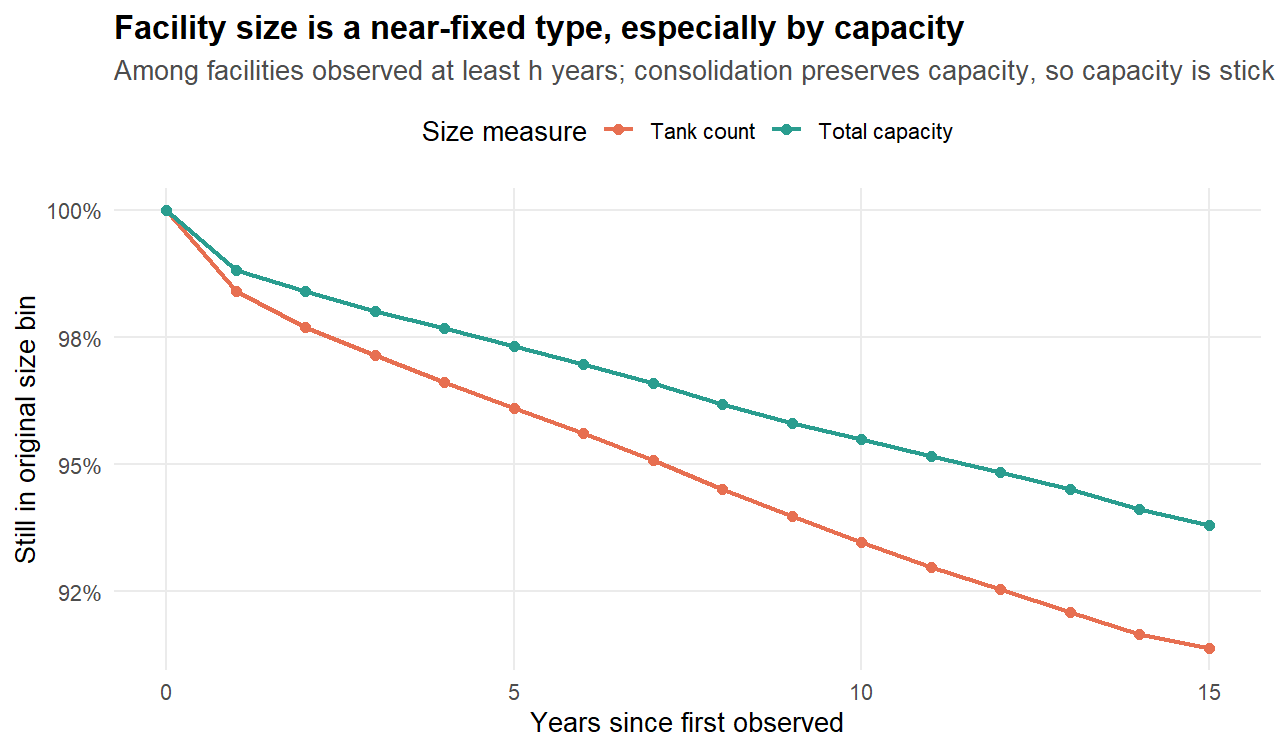
\includegraphics[width=0.78\textwidth,height=0.6\textheight,keepaspectratio]{../../Output/Figures/04ag_FixedType_Survival.png}
\end{center}

\vspace{0.05cm}

\centering\small\textit{The fixed-type test is not the one-year stay rate ($99\%$) --- size must stay put over a facility's whole spell (mean 16 yrs). It does: $\sim$\,92\% of facilities never change their \textbf{tank-count} bin and $\sim$\,94\% never change their \textbf{capacity} bin. Capacity is stickier (consolidation drops a tank but holds capacity), so it is the natural fixed-type size state --- entered with no transition to estimate.}

\begin{tikzpicture}[remember picture, overlay]
\node[anchor=south west, inner sep=0pt] at ([xshift=10pt, yshift=10pt]current page.south west) {%
  \navbutton[portfolio-limit][fill=BerkeleyBlue, font=\tiny, inner sep=2pt]{$\leftarrow$ back}%
};
\end{tikzpicture}
\end{frame}

\begin{frame}{Appendix: Within-facility homogeneity --- one tank
summarizes the rest}
\phantomsection\label{appendix-within-facility-homogeneity-one-tank-summarizes-the-rest}
\BerkeleyLightMode

\vspace{0.2cm}
\begin{center}
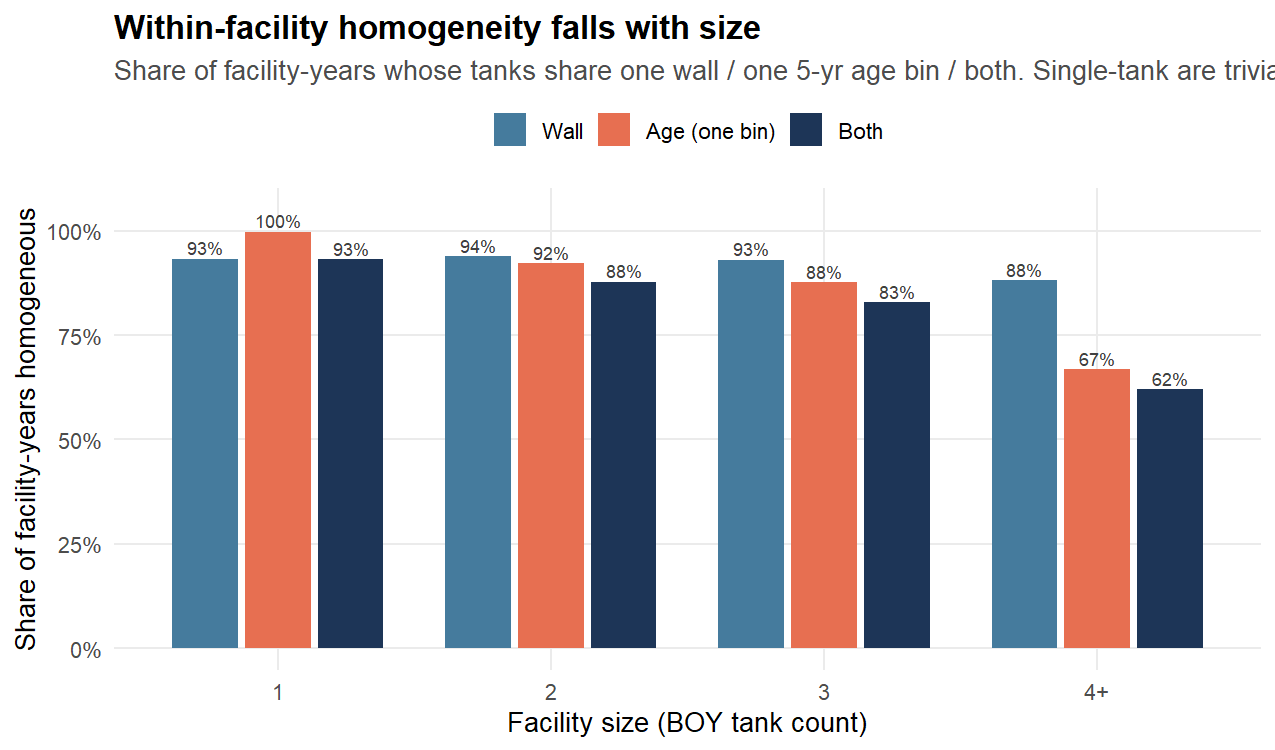
\includegraphics[width=0.82\textwidth,height=0.56\textheight,keepaspectratio]{../../Output/Figures/04ah_Homogeneity_bySize.png}
\end{center}

\vspace{0.05cm}

\centering\small\textit{The other half of ``size as a fixed type'': is one representative tank a faithful summary? Across facility-years, $81.5\%$ have all tanks in one wall type \emph{and} one 5-year age bin --- the exact support of the state. The median facility at every size has \emph{zero} age spread (tanks installed together); heterogeneity is an age-spread phenomenon that emerges only at \textbf{4+}-tank facilities ($62\%$ homogeneous). So the single representative tank is exact for the bulk of facility-years --- the histogram earns its keep only in the large-facility tail.}

\begin{tikzpicture}[remember picture, overlay]
\node[anchor=south west, inner sep=0pt] at ([xshift=10pt, yshift=10pt]current page.south west) {%
  \navbutton[portfolio-limit][fill=BerkeleyBlue, font=\tiny, inner sep=2pt]{$\leftarrow$ back}%
};
\end{tikzpicture}
\end{frame}

\begin{frame}{Appendix: Which tank do they shed? The margin is
predictable}
\phantomsection\label{appendix-which-tank-do-they-shed-the-margin-is-predictable}
\BerkeleyLightMode

\vspace{0.2cm}
\begin{center}
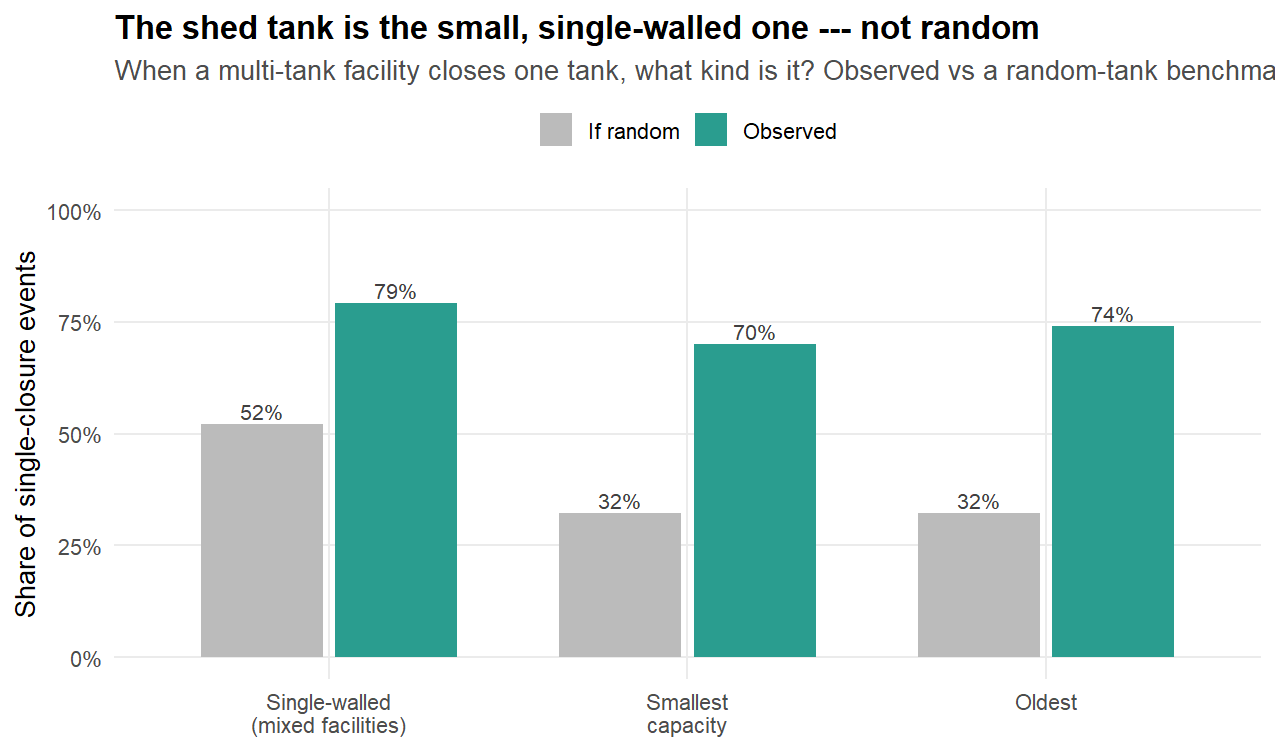
\includegraphics[width=0.82\textwidth,height=0.56\textheight,keepaspectratio]{../../Output/Figures/04ai_WhichTank_Shed.png}
\end{center}

\vspace{0.05cm}

\centering\small\textit{When a multi-tank facility closes \emph{one} tank, it is not random: it is the \textbf{single-walled} tank ($79\%$ in mixed facilities vs.\ $52\%$ by chance), the \textbf{smallest} ($70\%$ vs.\ $32\%$), and more weakly the oldest. So even at large heterogeneous facilities the acted-on tank is predictable --- the model can carry the portfolio with a \emph{marginal-tank} state (the small SW tank) and a capacity-preserving step-down transition, no full histogram needed.}

\begin{tikzpicture}[remember picture, overlay]
\node[anchor=south west, inner sep=0pt] at ([xshift=10pt, yshift=10pt]current page.south west) {%
  \navbutton[portfolio-limit][fill=BerkeleyBlue, font=\tiny, inner sep=2pt]{$\leftarrow$ back}%
};
\end{tikzpicture}
\end{frame}

\begin{frame}{Appendix: Choice probabilities fan out by facility size}
\phantomsection\label{appendix-choice-probabilities-fan-out-by-facility-size}
\BerkeleyLightMode

\hypertarget{portfolio-size}{}

\vspace{0.2cm}
\begin{center}
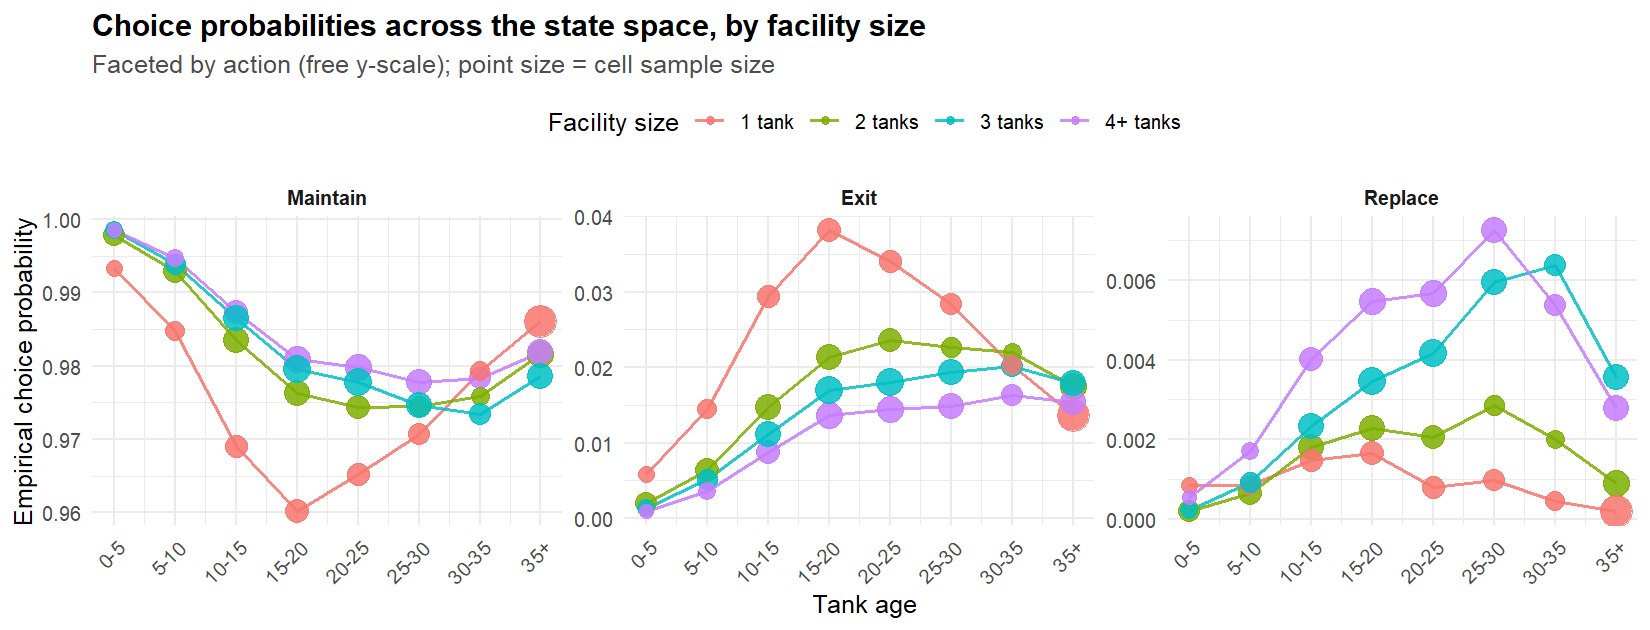
\includegraphics[width=0.82\textwidth,height=0.5\textheight,keepaspectratio]{../../Output/Figures/04u_CCP_by_Size.png}
\end{center}

\vspace{0.05cm}

\centering\small\textit{Empirical choice probabilities by facility size (point size $=$ cell sample size). \textbf{Exit} concentrates at single-tank facilities; \textbf{``replace''} concentrates at large facilities and \emph{young} tanks --- portfolio churn, not tanks wearing out. The single-tank model has one probability per cell and cannot represent this spread.}

\begin{tikzpicture}[remember picture, overlay]
\node[anchor=south west, inner sep=0pt] at ([xshift=10pt, yshift=10pt]current page.south west) {%
  \navbutton[portfolio-limit][fill=BerkeleyBlue, font=\tiny, inner sep=2pt]{$\leftarrow$ back}%
};
\end{tikzpicture}
\end{frame}

\begin{frame}{Appendix: Single-walled CCPs across regimes}
\phantomsection\label{appendix-single-walled-ccps-across-regimes}
\BerkeleyLightMode

\hypertarget{portfolio-ccp-sw}{}

\vspace{0.2cm}
\begin{center}
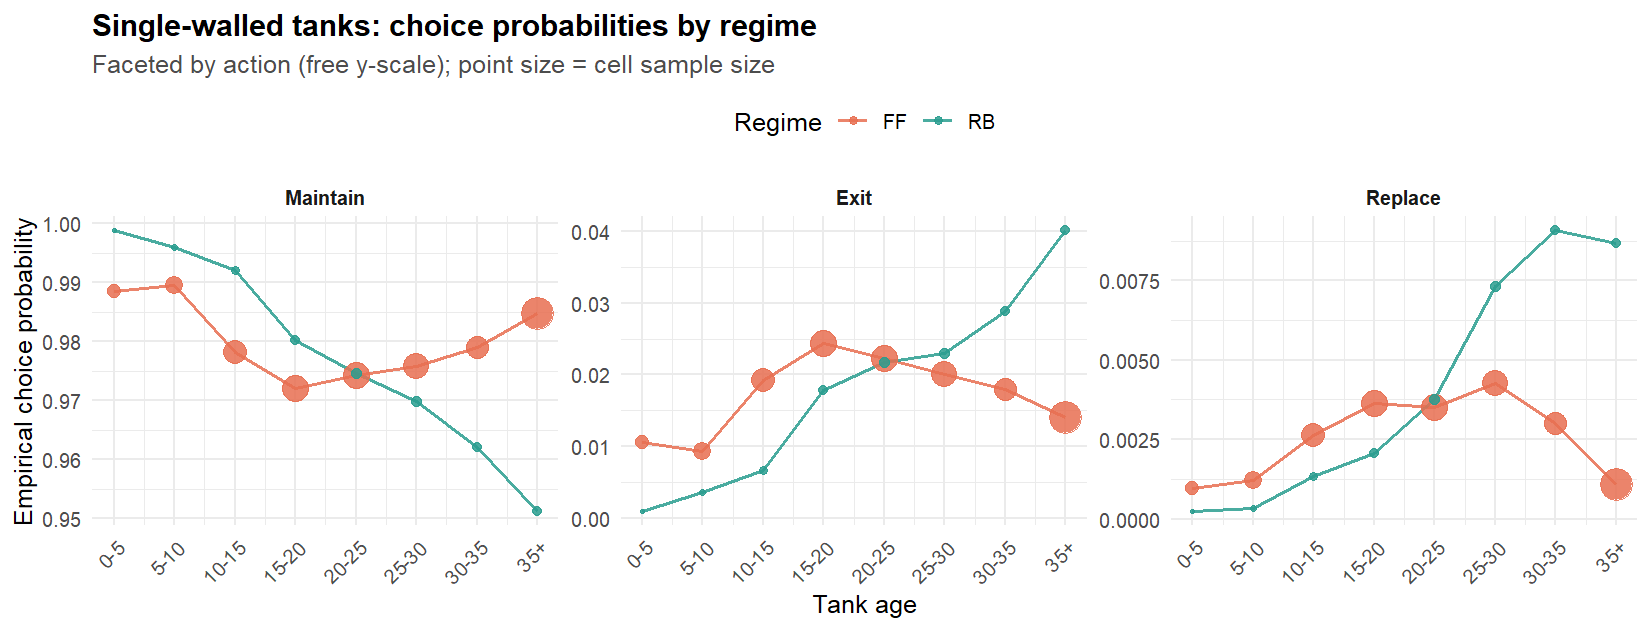
\includegraphics[width=0.82\textwidth,height=0.5\textheight,keepaspectratio]{../../Output/Figures/04u_CCP_SW_byRegime.png}
\end{center}

\vspace{0.05cm}

\centering\small\textit{Single-walled tanks, flat-fee vs.\ risk-based. Under risk-based pricing, exit rises steeply at old ages (middle panel) --- the premium channel the structural model captures cleanly.}

\begin{tikzpicture}[remember picture, overlay]
\node[anchor=south west, inner sep=0pt] at ([xshift=10pt, yshift=10pt]current page.south west) {%
  \navbutton[portfolio-limit][fill=BerkeleyBlue, font=\tiny, inner sep=2pt]{$\leftarrow$ back}%
};
\end{tikzpicture}
\end{frame}

\begin{frame}{Appendix: Double-walled CCPs across regimes}
\phantomsection\label{appendix-double-walled-ccps-across-regimes}
\BerkeleyLightMode

\hypertarget{portfolio-ccp-dw}{}

\vspace{0.2cm}
\begin{center}
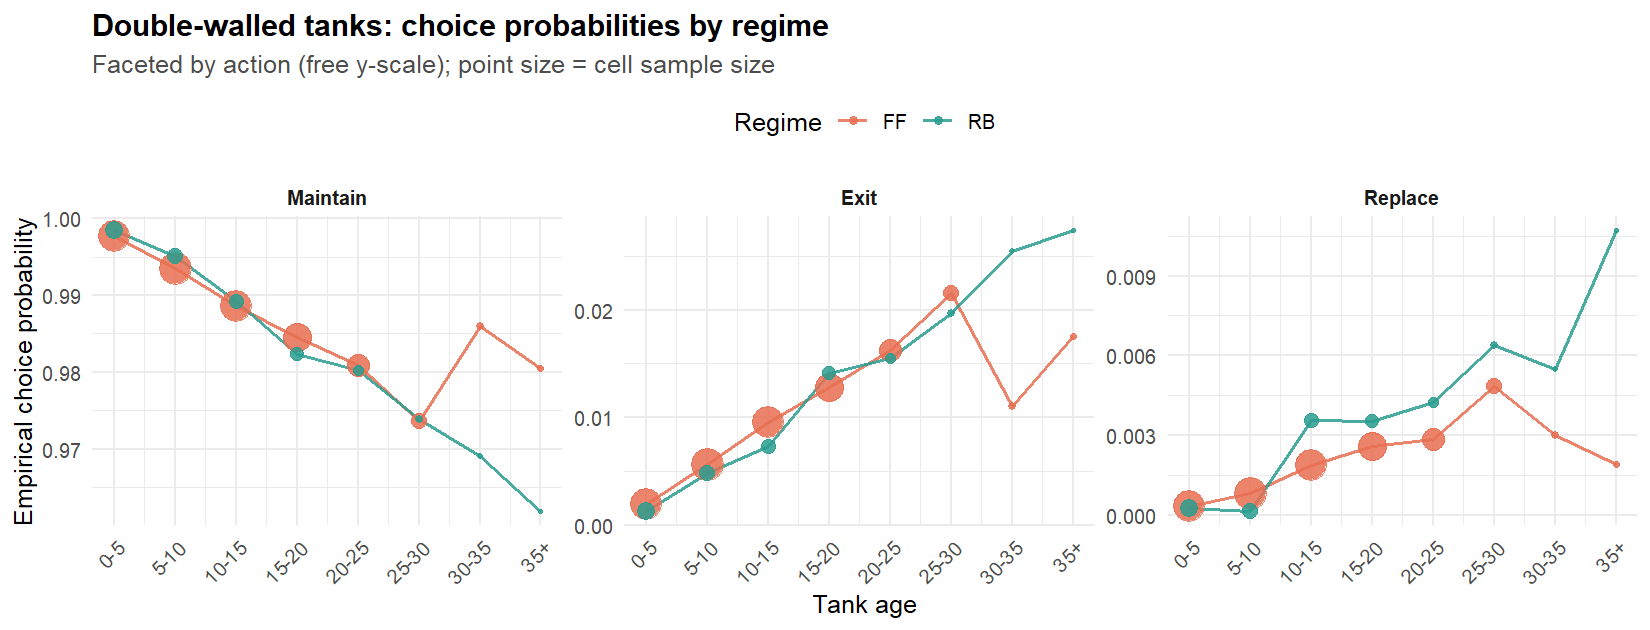
\includegraphics[width=0.82\textwidth,height=0.5\textheight,keepaspectratio]{../../Output/Figures/04u_CCP_DW_byRegime.png}
\end{center}

\vspace{0.05cm}

\centering\small\textit{Double-walled tanks, flat-fee vs.\ risk-based (canonical estimation-panel coding). Both exit and replacement rise with tank age; risk-based pricing steepens the old-age response.}

\begin{tikzpicture}[remember picture, overlay]
\node[anchor=south west, inner sep=0pt] at ([xshift=10pt, yshift=10pt]current page.south west) {%
  \navbutton[portfolio-limit][fill=BerkeleyBlue, font=\tiny, inner sep=2pt]{$\leftarrow$ back}%
};
\end{tikzpicture}
\end{frame}

\begin{frame}{Appendix: Where closures go, by facility size}
\phantomsection\label{appendix-where-closures-go-by-facility-size}
\BerkeleyLightMode

\hypertarget{portfolio-replace}{}

\vspace{0.2cm}
\begin{center}
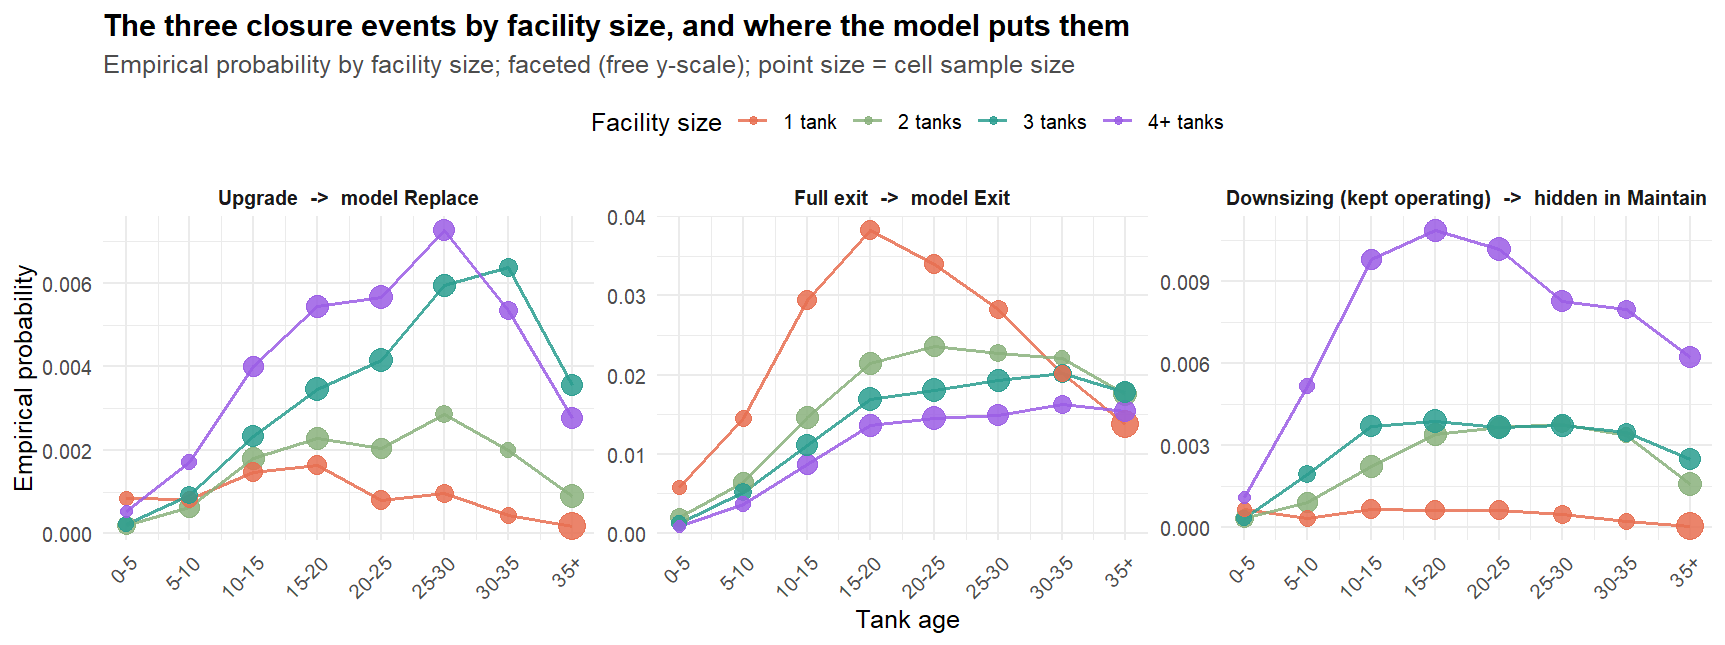
\includegraphics[width=0.86\textwidth,height=0.52\textheight,keepaspectratio]{../../Output/Figures/04w_Replace_Decomp.png}
\end{center}

\vspace{0.05cm}

\centering\small\textit{The three closure events by facility size. Upgrades $\to$ Replace (left) and full exits $\to$ Exit (middle) are coded correctly. \textbf{Downsizing} (right; closed a tank but kept operating) is hidden in Maintain --- and it rises sharply with facility size, the omitted-state (portfolio) problem. \emph{Note the differing $y$-scales.}}

\begin{tikzpicture}[remember picture, overlay]
\node[anchor=south west, inner sep=0pt] at ([xshift=10pt, yshift=10pt]current page.south west) {%
  \navbutton[portfolio-limit][fill=BerkeleyBlue, font=\tiny, inner sep=2pt]{$\leftarrow$ back}%
  \hspace{3pt}%
  \navbutton[portfolio-maintain][fill=BerkeleyBlue, font=\tiny, inner sep=2pt]{Maintain decomp $\rightarrow$}%
};
\end{tikzpicture}
\end{frame}

\begin{frame}{Appendix: Where closures go, by regime (FF vs.~RB)}
\phantomsection\label{appendix-where-closures-go-by-regime-ff-vs.-rb}
\BerkeleyLightMode

\hypertarget{portfolio-replace-regime}{}

\vspace{0.2cm}
\begin{center}
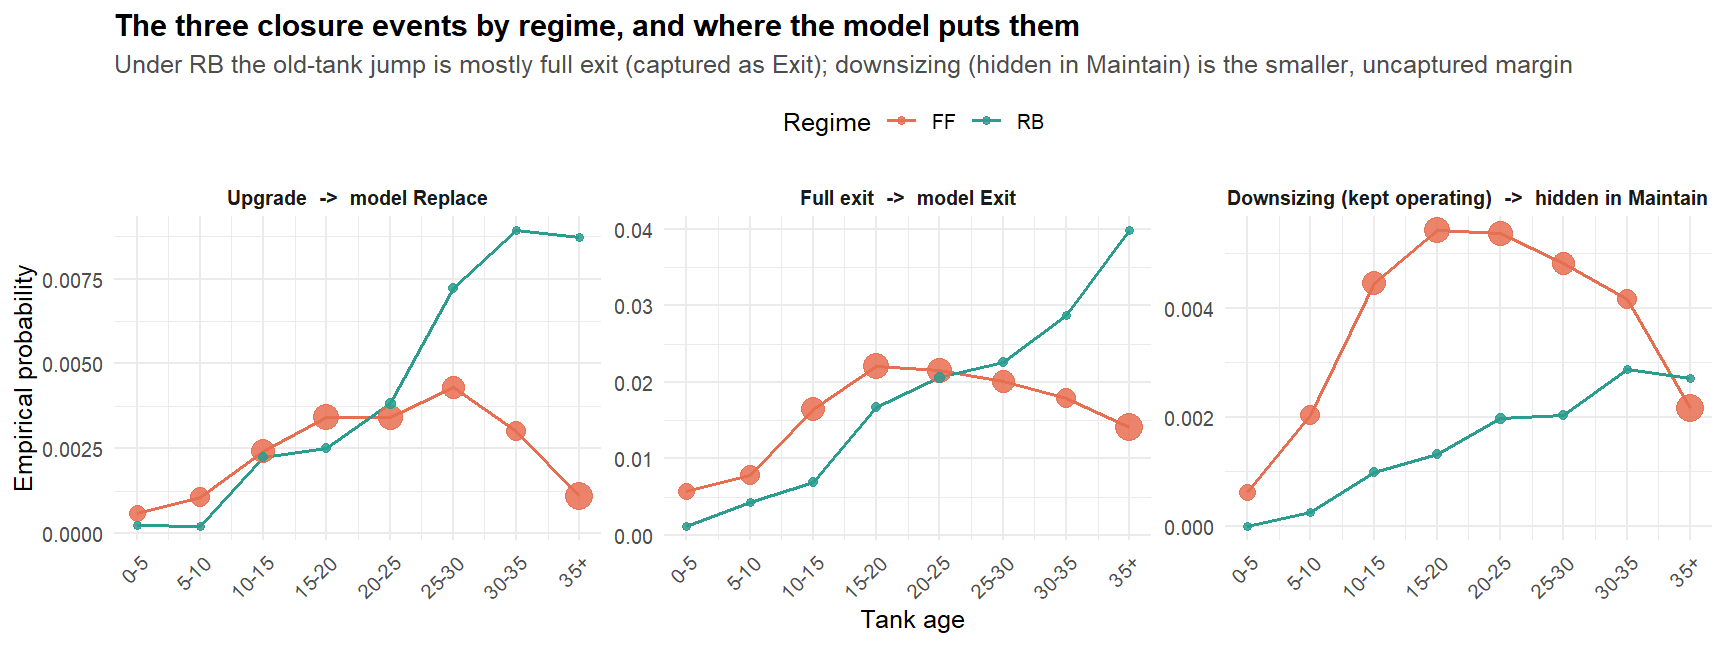
\includegraphics[width=0.86\textwidth,height=0.52\textheight,keepaspectratio]{../../Output/Figures/04y_Replace_Decomp_byRegime.png}
\end{center}

\vspace{0.05cm}

\centering\small\textit{The same three events, split by regime. Under risk-based pricing the old-tank jump is mostly \textbf{full exit} (middle; coded Exit --- captured cleanly). \textbf{Downsizing} (right; hidden in Maintain) is the smaller, uncaptured margin --- and is not even RB-driven. The model captures the dominant RB response; the gap is the partial-downsizing margin.}

\begin{tikzpicture}[remember picture, overlay]
\node[anchor=south west, inner sep=0pt] at ([xshift=10pt, yshift=10pt]current page.south west) {%
  \navbutton[portfolio-limit][fill=BerkeleyBlue, font=\tiny, inner sep=2pt]{$\leftarrow$ back}%
  \hspace{3pt}%
  \navbutton[portfolio-replace-fit][fill=BerkeleyBlue, font=\tiny, inner sep=2pt]{Model fit $\rightarrow$}%
};
\end{tikzpicture}
\end{frame}

\begin{frame}{Appendix: Model fit --- Exit (the margin that matters)}
\phantomsection\label{appendix-model-fit-exit-the-margin-that-matters}
\BerkeleyLightMode

\vspace{0.1cm}
\begin{center}
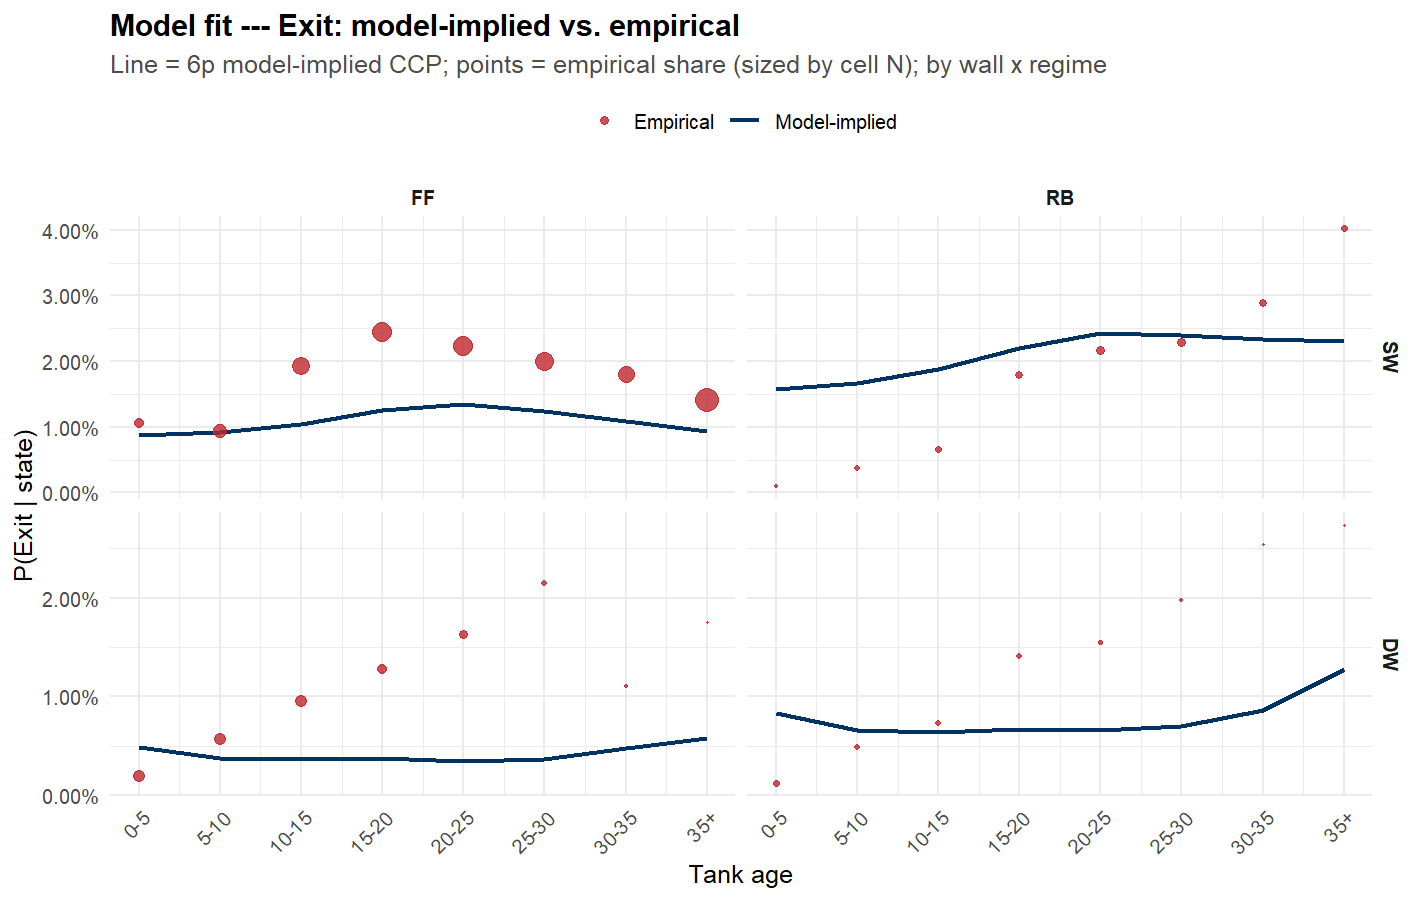
\includegraphics[width=0.78\textwidth,height=0.62\textheight,keepaspectratio]{../../Output/Figures/04ad_ModelFit_Exit.png}
\end{center}

\vspace{0.05cm}

\centering\small\textit{Exit is the dominant non-maintain action (1.7\% of years) and the channel the welfare results run through. The model captures its shape --- rising with age, higher under RB at old tanks --- though it undershoots single-walled flat-fee exit at mid-ages.}

\begin{tikzpicture}[remember picture, overlay]
\node[anchor=south west, inner sep=0pt] at ([xshift=10pt, yshift=10pt]current page.south west) {%
  \navbutton[portfolio-limit][fill=BerkeleyBlue, font=\tiny, inner sep=2pt]{$\leftarrow$ back}%
};
\end{tikzpicture}
\end{frame}

\begin{frame}{Appendix: Model fit --- Maintain}
\phantomsection\label{appendix-model-fit-maintain}
\BerkeleyLightMode

\vspace{0.1cm}
\begin{center}
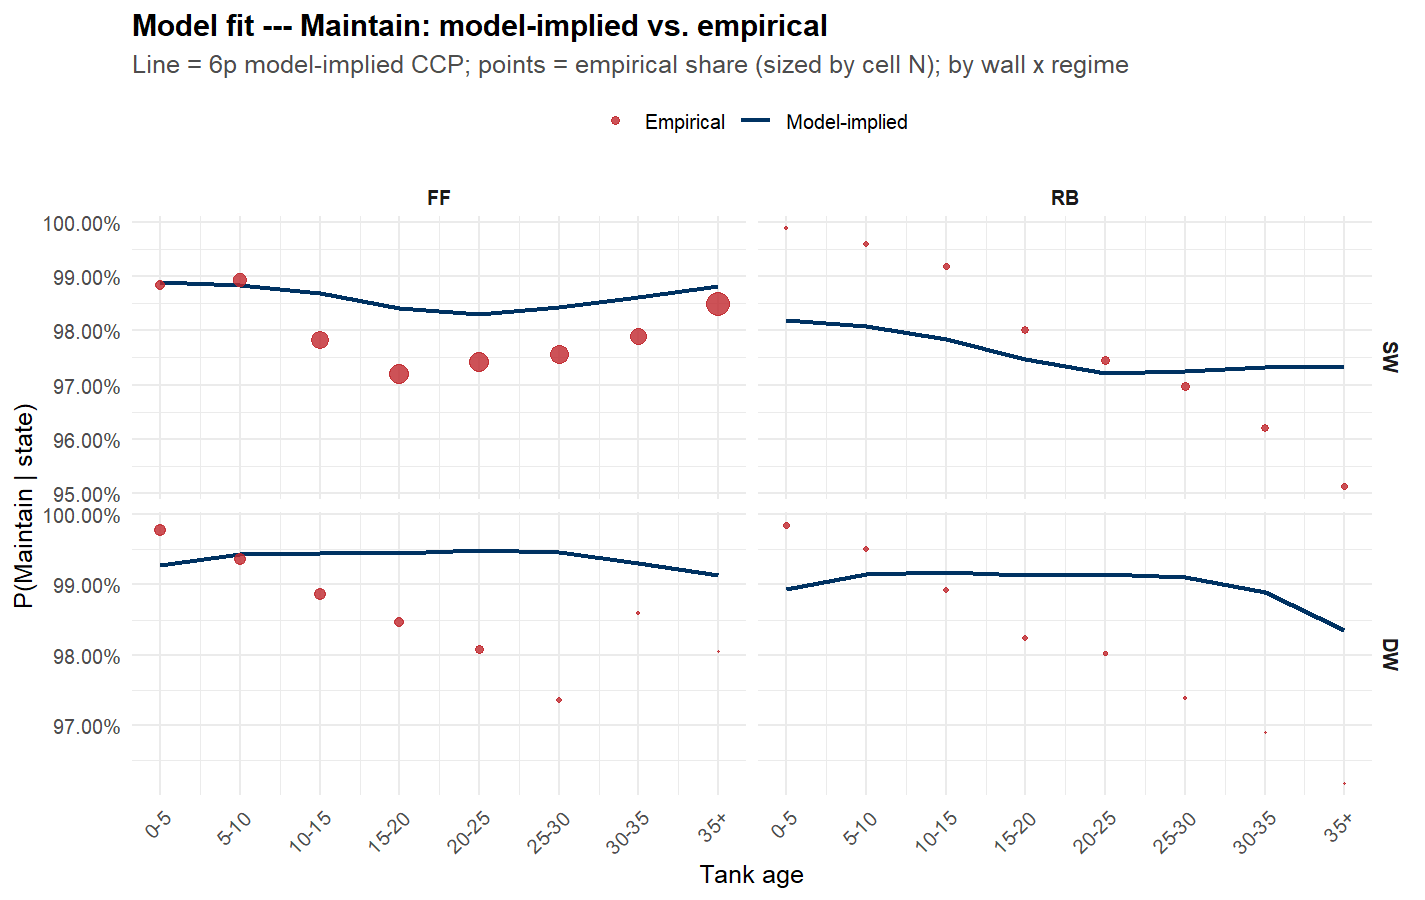
\includegraphics[width=0.78\textwidth,height=0.62\textheight,keepaspectratio]{../../Output/Figures/04ad_ModelFit_Maintain.png}
\end{center}

\begin{tikzpicture}[remember picture, overlay]
\node[anchor=south west, inner sep=0pt] at ([xshift=10pt, yshift=10pt]current page.south west) {%
  \navbutton[portfolio-limit][fill=BerkeleyBlue, font=\tiny, inner sep=2pt]{$\leftarrow$ back}%
};
\end{tikzpicture}
\end{frame}

\begin{frame}{Appendix: Model fit --- Replace (rare, low-stakes)}
\phantomsection\label{appendix-model-fit-replace-rare-low-stakes}
\BerkeleyLightMode

\hypertarget{portfolio-replace-fit}{}

\vspace{0.1cm}
\begin{center}
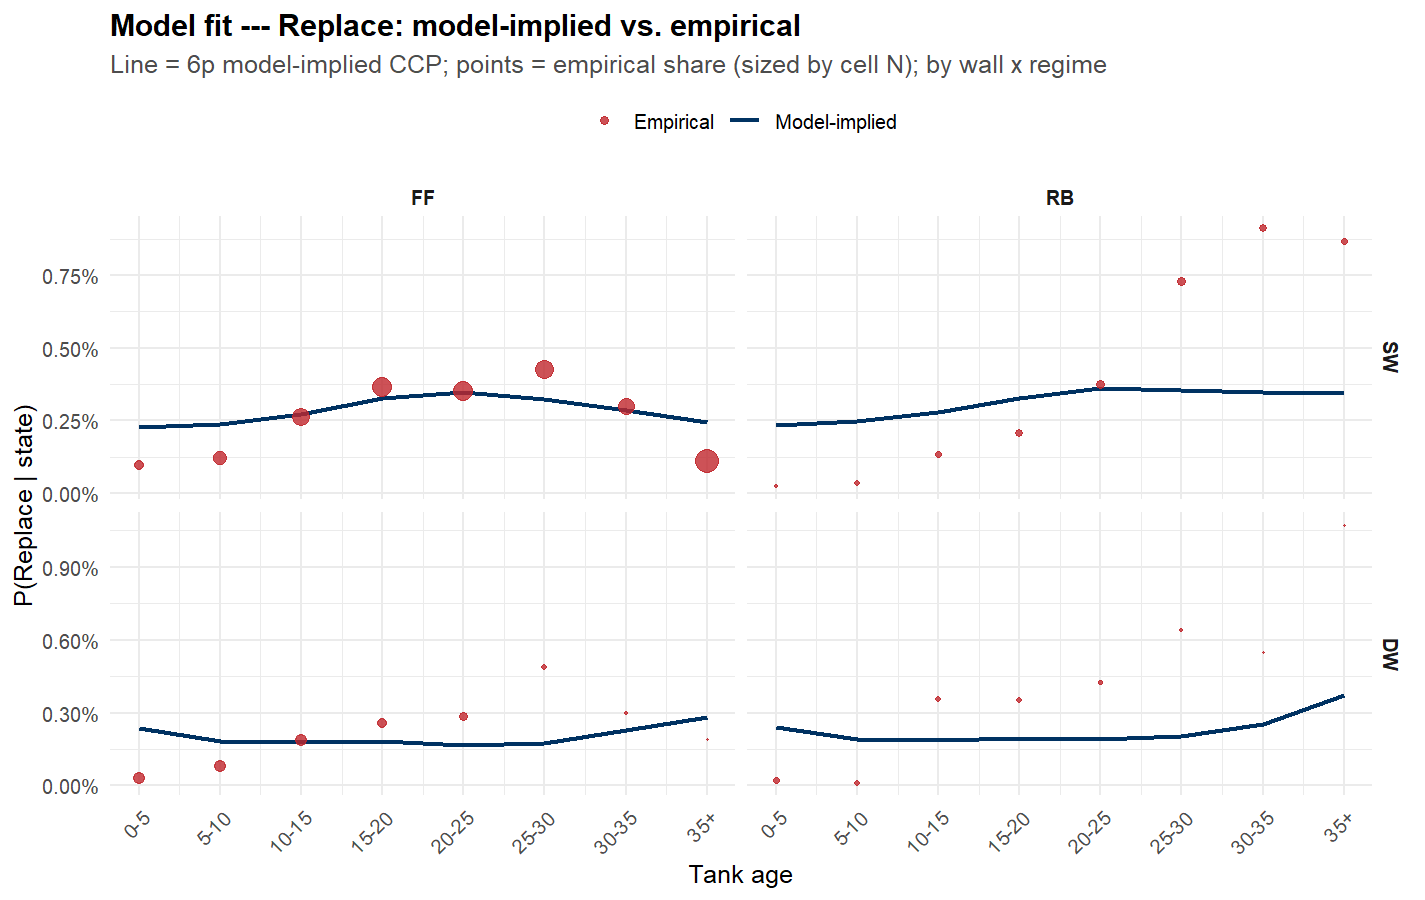
\includegraphics[width=0.78\textwidth,height=0.62\textheight,keepaspectratio]{../../Output/Figures/04ad_ModelFit_Replace.png}
\end{center}

\vspace{0.05cm}

\centering\small\textit{Replace is only $0.27\%$ of years. The model smooths the empirical old-RB bump (e.g.\ SW-RB reaches $\sim$\,0.9\% at 35+ vs a model line near $0.35\%$), but because the action is so rare this has little leverage on the estimates --- \textbf{exit is the margin that matters, and it is captured.}}

\begin{tikzpicture}[remember picture, overlay]
\node[anchor=south west, inner sep=0pt] at ([xshift=10pt, yshift=10pt]current page.south west) {%
  \navbutton[portfolio-limit][fill=BerkeleyBlue, font=\tiny, inner sep=2pt]{$\leftarrow$ back}%
};
\end{tikzpicture}
\end{frame}

\begin{frame}{Appendix: What the model calls ``maintain'\,' --- hidden
partial closures}
\phantomsection\label{appendix-what-the-model-calls-maintain-hidden-partial-closures}
\BerkeleyLightMode

\hypertarget{portfolio-maintain}{}

\vspace{0.2cm}
\begin{center}
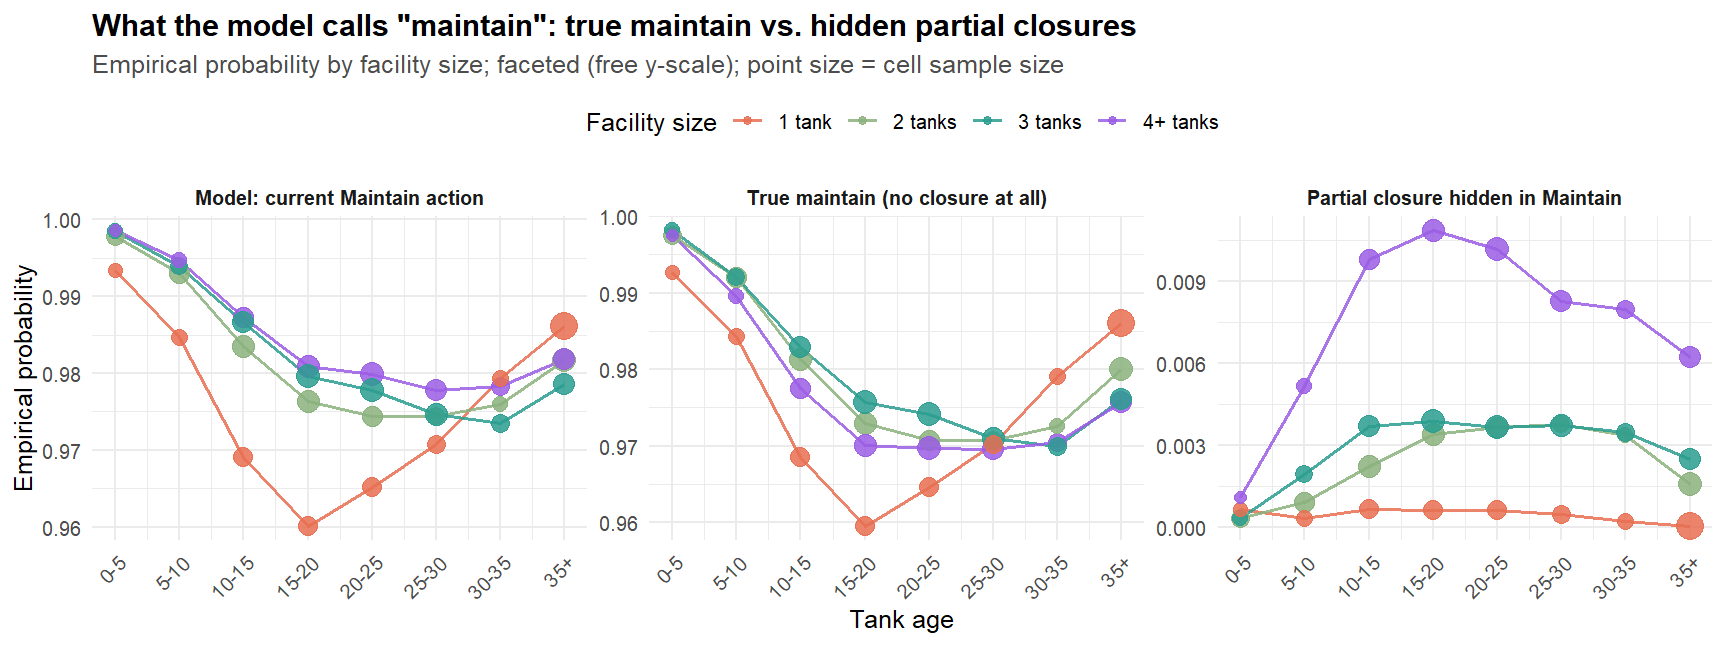
\includegraphics[width=0.86\textwidth,height=0.52\textheight,keepaspectratio]{../../Output/Figures/04w_Maintain_Decomp.png}
\end{center}

\vspace{0.05cm}

\centering\small\textit{Almost all of ``maintain'' is genuine (left $\approx$ middle). The sliver that is not is \textbf{partial closures} --- a facility dropped a tank but kept operating, so it is coded maintain (right). That sliver \emph{scales with facility size}: $\sim$\,1.1\% per year at 4+-tank facilities vs.\ $\sim$\,0.05\% at single-tank facilities. The margin the model misses is, mechanically, a \textbf{size} dimension.}

\begin{tikzpicture}[remember picture, overlay]
\node[anchor=south west, inner sep=0pt] at ([xshift=10pt, yshift=10pt]current page.south west) {%
  \navbutton[portfolio-limit][fill=BerkeleyBlue, font=\tiny, inner sep=2pt]{$\leftarrow$ back}%
};
\end{tikzpicture}
\end{frame}

\begin{frame}{Appendix: At ``replace'\,' events, facilities shed tanks}
\phantomsection\label{appendix-at-replace-events-facilities-shed-tanks}
\BerkeleyLightMode

\hypertarget{portfolio-hist}{}

\vspace{0.05cm}
\begin{center}
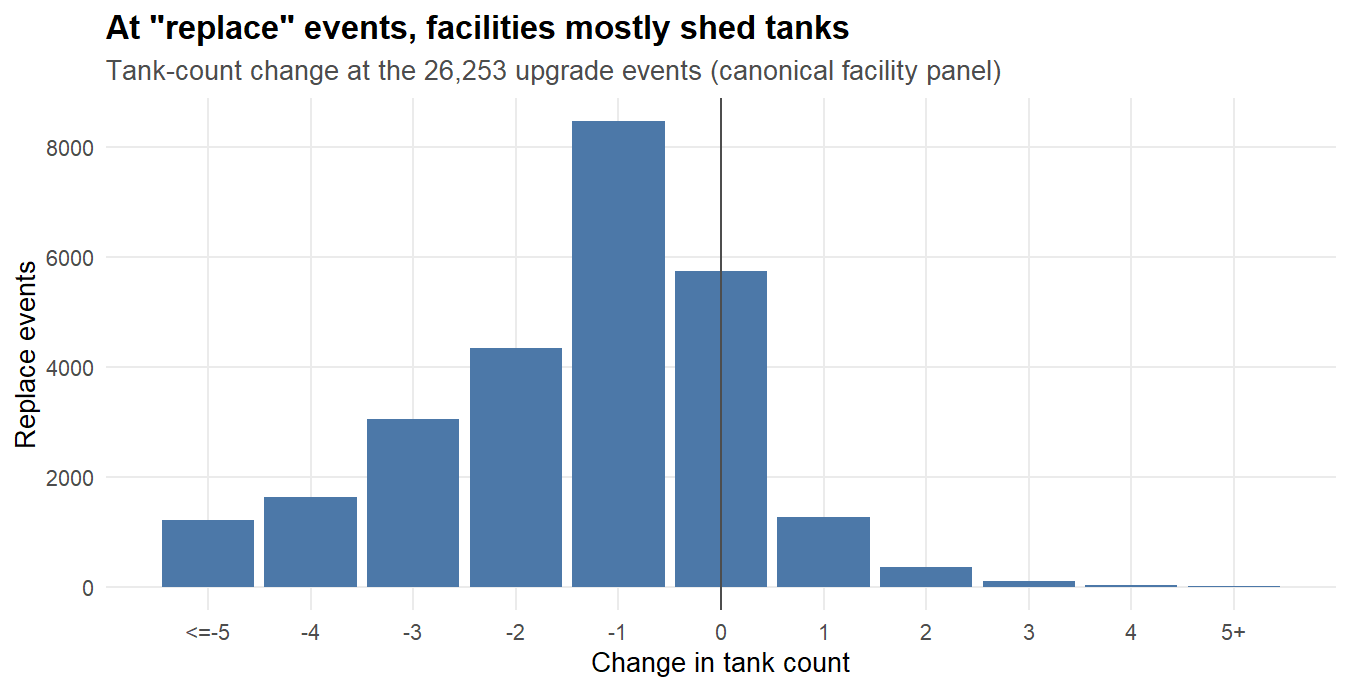
\includegraphics[width=0.66\textwidth,height=0.37\textheight,keepaspectratio]{../../Output/Figures/04ac_ReplaceTankChange_Hist.png}

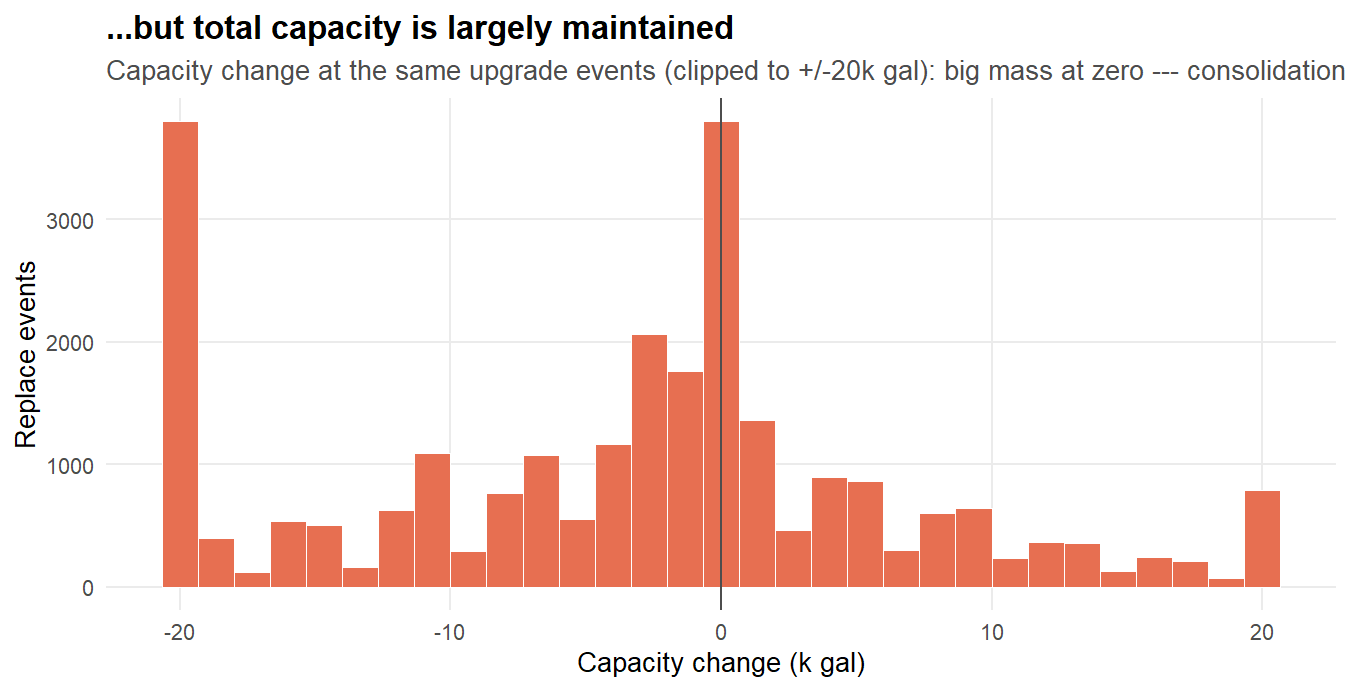
\includegraphics[width=0.66\textwidth,height=0.37\textheight,keepaspectratio]{../../Output/Figures/04ac_ReplaceCapChange_Hist.png}
\end{center}

\vspace{0.05cm}

\centering\small\textit{At the 26{,}253 ``replace'' events: tank count mostly \emph{falls} (top), yet total capacity is largely \emph{maintained} (bottom). So the common changes ($0$ and $-1$ tanks) are \textbf{consolidations} --- fewer, larger tanks --- not the single-tank reset the model assumes.}

\begin{tikzpicture}[remember picture, overlay]
\node[anchor=south west, inner sep=0pt] at ([xshift=10pt, yshift=10pt]current page.south west) {%
  \navbutton[portfolio-limit][fill=BerkeleyBlue, font=\tiny, inner sep=2pt]{$\leftarrow$ back}%
};
\end{tikzpicture}
\end{frame}

\begin{frame}{Appendix: Tank loss and capacity loss move together}
\phantomsection\label{appendix-tank-loss-and-capacity-loss-move-together}
\BerkeleyLightMode

\hypertarget{portfolio-cov}{}

\vspace{0.1cm}
\begin{center}
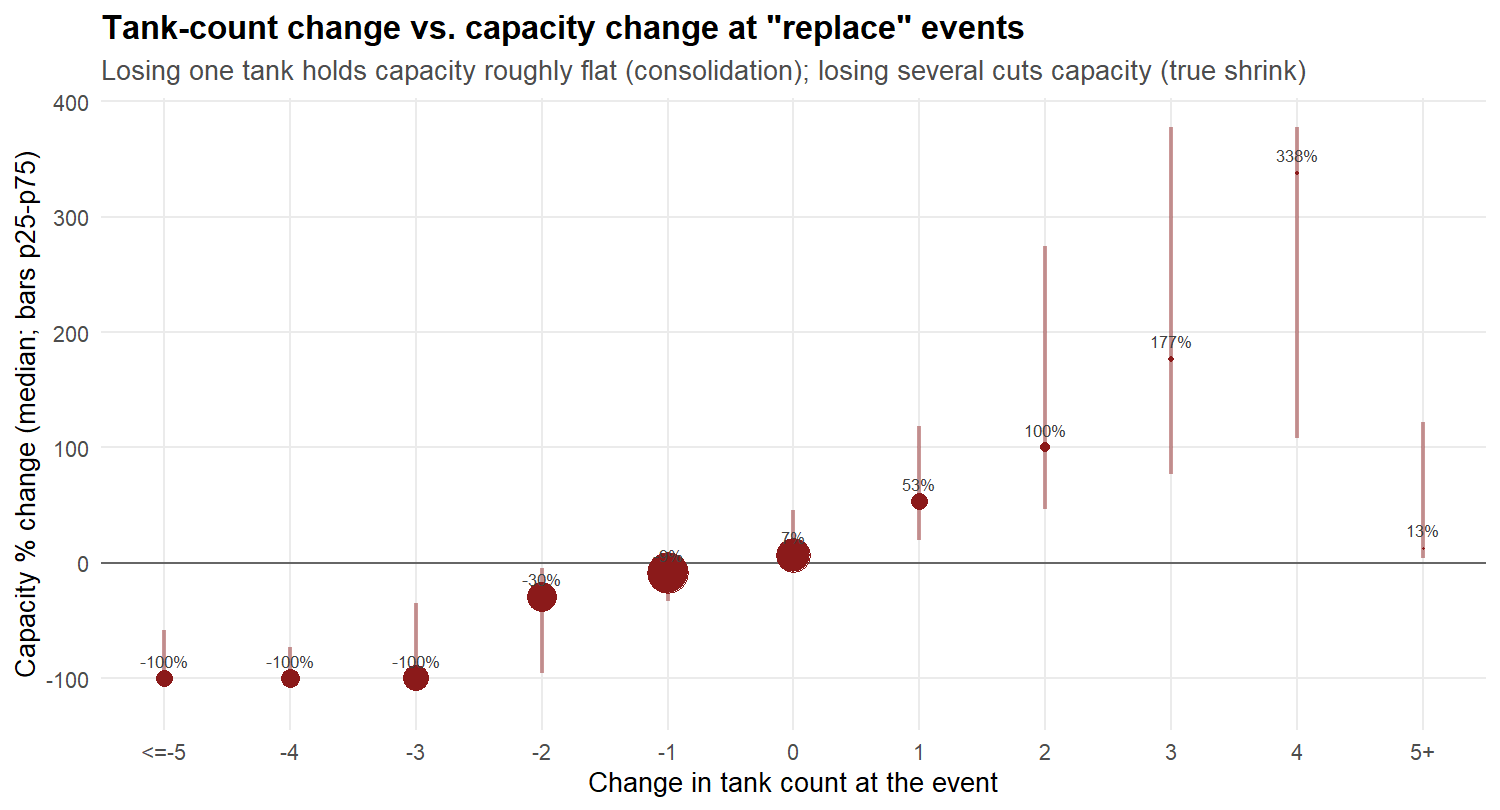
\includegraphics[width=0.9\textwidth,height=0.6\textheight,keepaspectratio]{../../Output/Figures/04ac_ReplaceTankVsCapacity_BinScatter.png}
\end{center}

\vspace{0.05cm}

\centering\small\textit{Capacity change vs.\ tank-count change at ``replace'' events. Losing one tank holds capacity roughly flat (consolidation --- fewer, larger tanks); losing several cuts capacity sharply (true shrinking). Either way the facility is \emph{resized}, not reset to one new tank.}

\begin{tikzpicture}[remember picture, overlay]
\node[anchor=south west, inner sep=0pt] at ([xshift=10pt, yshift=10pt]current page.south west) {%
  \navbutton[portfolio-limit][fill=BerkeleyBlue, font=\tiny, inner sep=2pt]{$\leftarrow$ back}%
};
\end{tikzpicture}
\end{frame}

\begin{frame}{Appendix: Downsizing corrupts the state, not just the
action}
\phantomsection\label{appendix-downsizing-corrupts-the-state-not-just-the-action}
\BerkeleyLightMode

\hypertarget{portfolio-offsupport}{}

\vspace{0.15cm}
\begin{center}
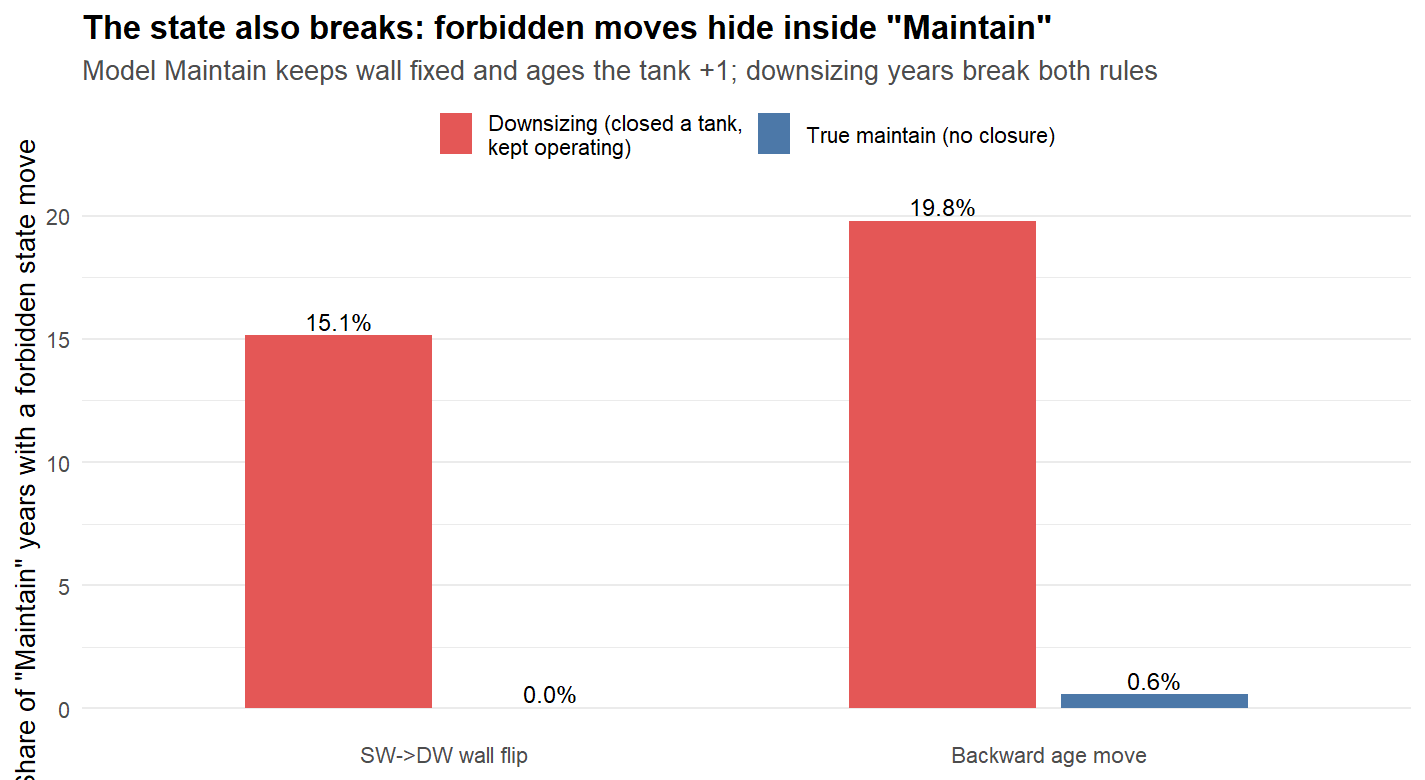
\includegraphics[width=0.85\textwidth,height=0.6\textheight,keepaspectratio]{../../Output/Figures/04ab_StateViolations_inMaintain.png}
\end{center}

\vspace{0.05cm}

\centering\small\textit{Model Maintain holds wall fixed and ages the tank $+1$. The downsizing years coded Maintain break both: $\sim$\,15\% flip \textbf{SW$\to$DW} (drop the SW tank, only DW remains --- 65\% of these flips closed an SW tank) and $\sim$\,20\% jump \emph{backward} in age (drop the oldest tank). True maintains do neither. The off-support transitions are not just a mislabeled action --- the state itself moves where Maintain forbids.}

\begin{tikzpicture}[remember picture, overlay]
\node[anchor=south west, inner sep=0pt] at ([xshift=10pt, yshift=10pt]current page.south west) {%
  \navbutton[portfolio-limit][fill=BerkeleyBlue, font=\tiny, inner sep=2pt]{$\leftarrow$ back}%
};
\end{tikzpicture}
\end{frame}

\begin{frame}{Appendix: Does the reduced form share this problem?}
\phantomsection\label{appendix-does-the-reduced-form-share-this-problem}
\BerkeleyLightMode

\textbf{No --- the reduced form is facility-level and portfolio-aware.}
It splits closures into three separate, well-defined facility outcomes:

\begin{itemize}
  \item \textbf{Full exit} --- the facility disappears; all tanks gone.
  \item \textbf{Upgrade} --- a tank closed \emph{and} a new tank installed the same year.
  \item \textbf{Shrink} --- a tank removed with \emph{no} install; the facility keeps operating, smaller.
\end{itemize}

A facility can be coded as \emph{both} upgrade and shrink in one year.
None of these impose a single-tank reset.

\vfill

\centering\small\textit{So the reduced-form ``composition shifts toward replacement'' result is sound. The single-tank reset that misses 98\% of replacements is specific to the structural model.}

\begin{tikzpicture}[remember picture, overlay]
\node[anchor=south west, inner sep=0pt] at ([xshift=10pt, yshift=10pt]current page.south west) {%
  \navbutton[portfolio-limit][fill=BerkeleyBlue, font=\tiny, inner sep=2pt]{$\leftarrow$ back}%
};
\end{tikzpicture}
\end{frame}

\begin{frame}{Appendix: TX-on-FF counterfactual --- SW action shares}
\phantomsection\label{appendix-tx-on-ff-counterfactual-sw-action-shares}
\BerkeleyLightMode

\hypertarget{cf-overlay-sw}{}

\vspace{0.2cm}
\begin{center}
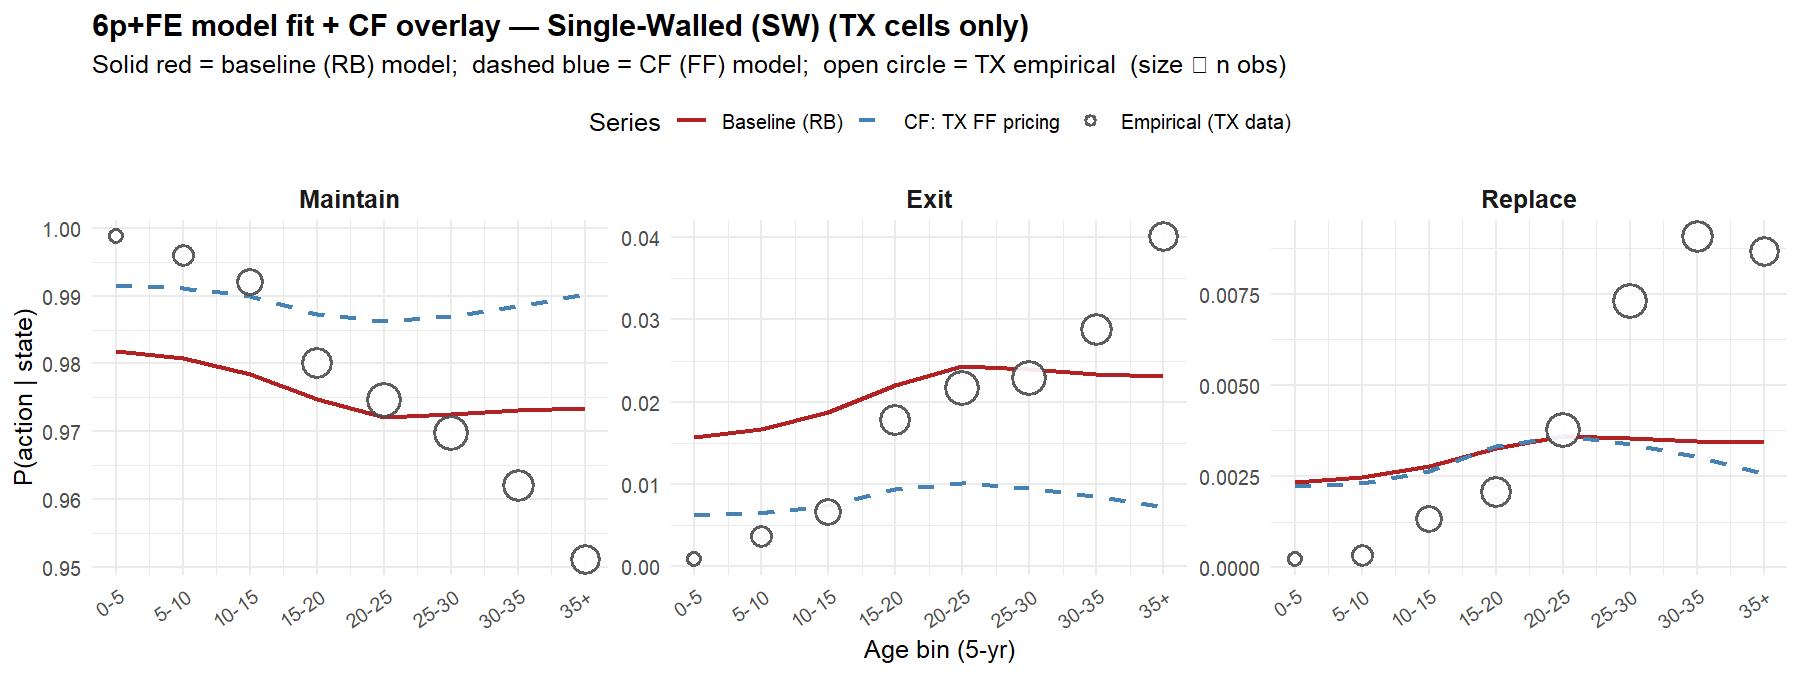
\includegraphics[width=0.92\textwidth,height=0.78\textheight,keepaspectratio]{../../Output/Figures/04o_Fit_6p_CF_Overlay_SW.png}
\end{center}
\end{frame}

\begin{frame}{Appendix: TX-on-FF counterfactual --- DW action shares}
\phantomsection\label{appendix-tx-on-ff-counterfactual-dw-action-shares}
\BerkeleyLightMode

\hypertarget{cf-overlay-dw}{}

\vspace{0.2cm}
\begin{center}
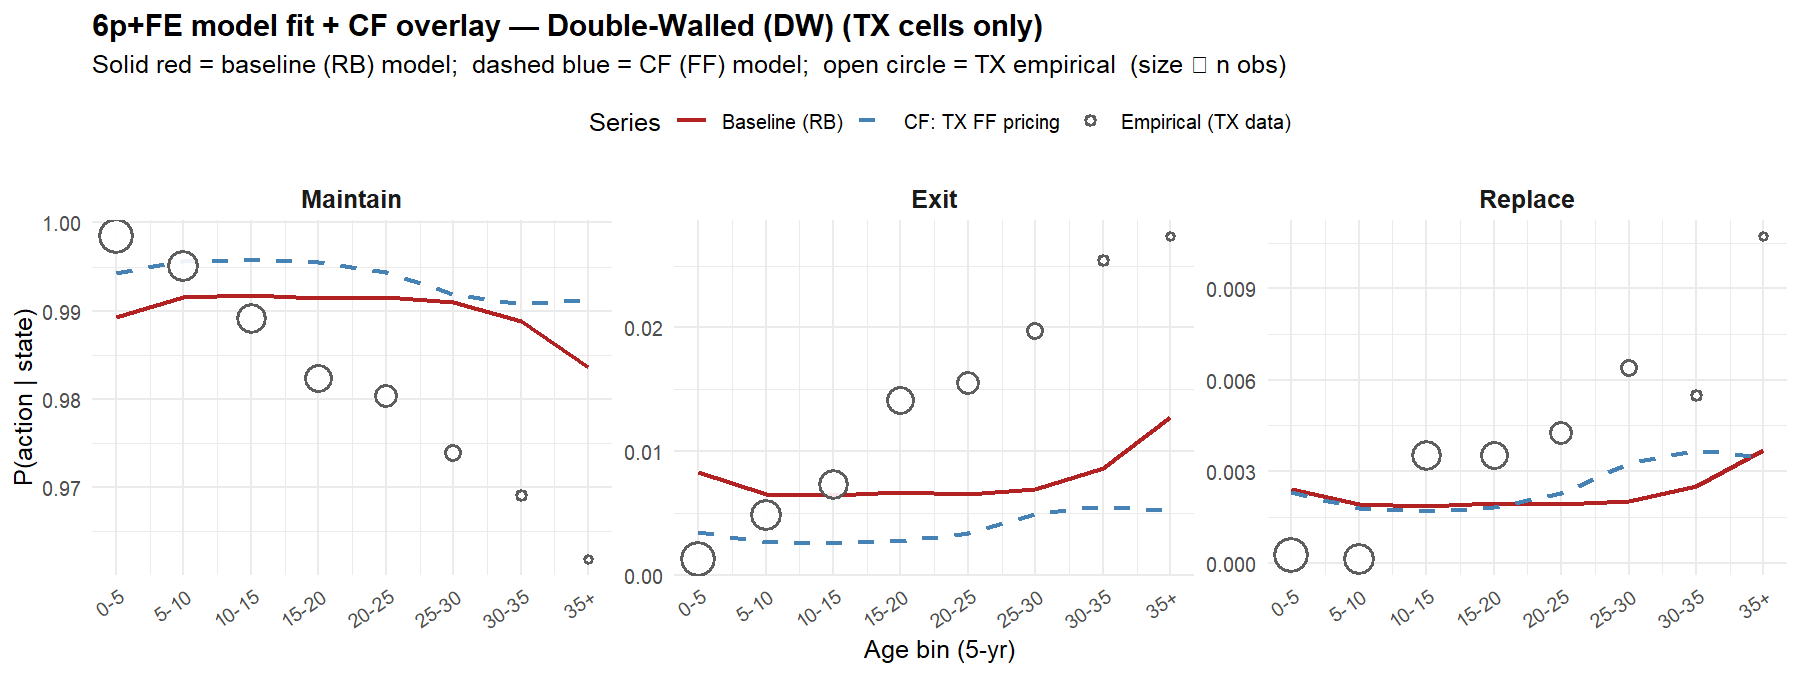
\includegraphics[width=0.92\textwidth,height=0.78\textheight,keepaspectratio]{../../Output/Figures/04o_Fit_6p_CF_Overlay_DW.png}
\end{center}
\end{frame}

\begin{frame}{Appendix: TX-on-FF counterfactual --- removal-age
distribution}
\phantomsection\label{appendix-tx-on-ff-counterfactual-removal-age-distribution}
\BerkeleyLightMode

\hypertarget{cf-removal-age}{}

\vspace{0.2cm}
\begin{center}
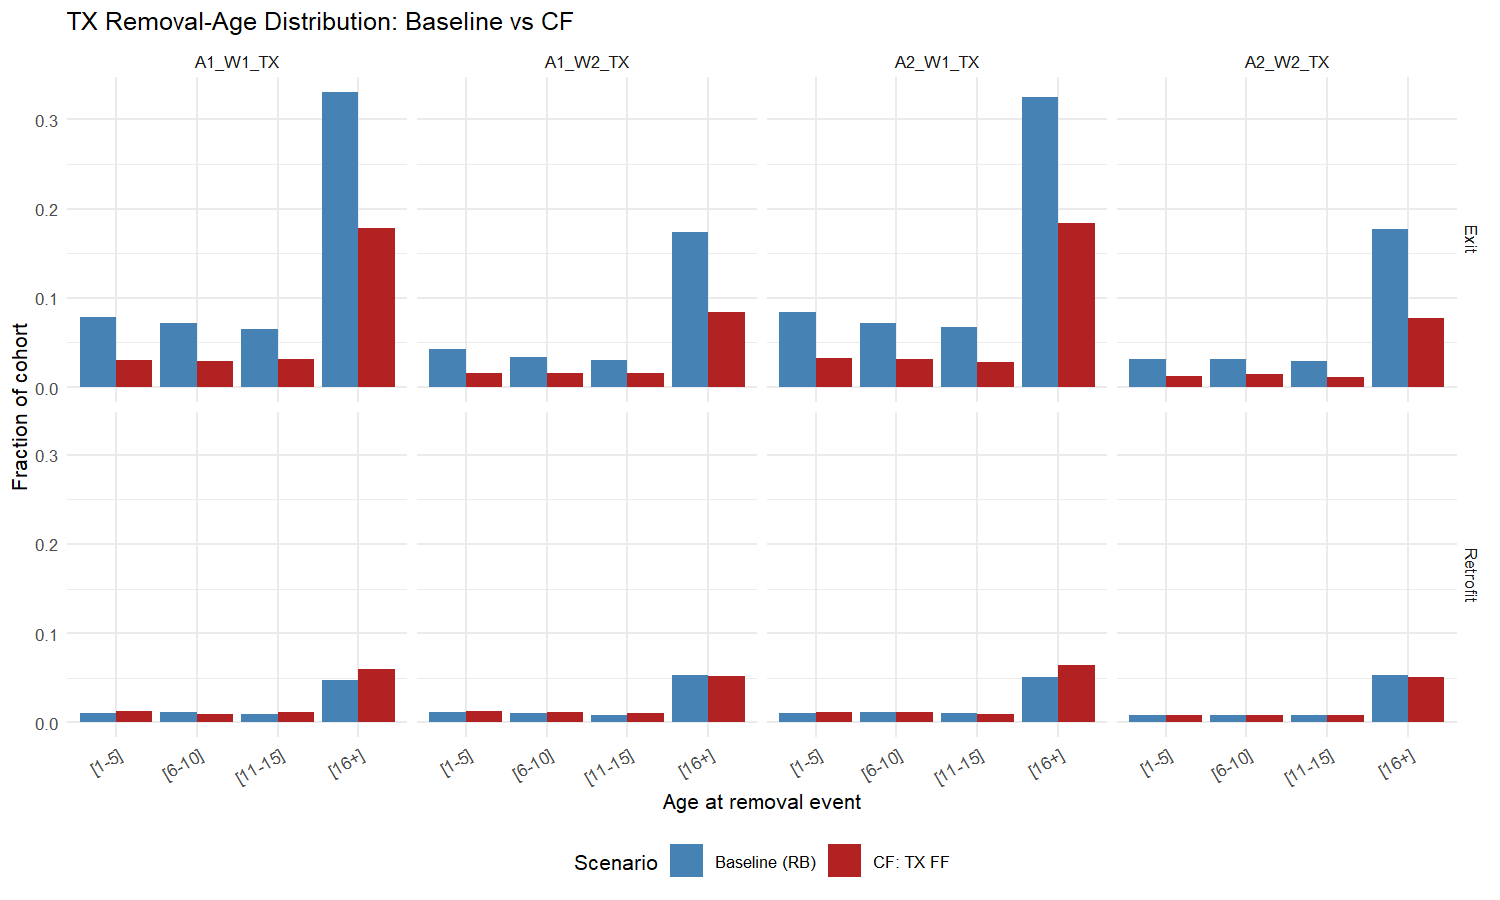
\includegraphics[width=0.92\textwidth,height=0.78\textheight,keepaspectratio]{../../Output/Figures/04o_CF_RemovalAge_Distribution_TX.png}
\end{center}
\end{frame}

\begin{frame}{A dynamic discrete-choice model of tank operations}
\phantomsection\label{a-dynamic-discrete-choice-model-of-tank-operations-1}
\BerkeleyLightMode

\textbf{Scale-incorporation model.} A facility is a \emph{portfolio} of
tanks, not one representative tank.

\begin{itemize}
\tightlist
\item
  \textbf{State} \(s=(n,\,G,\,\rho)\): tank counts \(n\) over 16
  categories (wall \(\times\) 8 age bins), capacity quartile \(G\),
  fixed regime \(\rho\)
\item
  Each period, choose from the menu \((k,m)\) --- remove \(k\) tanks
  (where \(0 \le k \le n\)), install \(m\) new ones:

  \begin{itemize}
  \tightlist
  \item
    \((0,0)\) \textbf{maintain} (keep all tanks)
  \item
    \((k,0)\) \textbf{downsize} (remove some tanks, \(0 < k < n\))
  \item
    \((k,m\ge 1)\) \textbf{replace/consolidate} (remove \(k\), install
    \(m\) newer ones)
  \item
    \(k=n\) \textbf{full exit} (exit the portfolio entirely)
  \end{itemize}
\item
  The choice trades the current flow payoff against the continuation
  value of the \emph{portfolio}
\end{itemize}

\vfill

\centering\small\textit{The single-tank model's keep / exit / replace becomes a per-unit-priced menu over the whole portfolio --- recovering the downsizing margin and the size-dependent regime response.}
\end{frame}

\begin{frame}{Flow utilities: one payoff per action}
\phantomsection\label{flow-utilities-one-payoff-per-action-1}
\BerkeleyLightMode

\begin{align*}
u_{(k,m)}(s) &= \estc{\varphi_G} + \alpha_g - \estc{\gamma_{\text{price}}}\,P(n',\rho) - \estc{\gamma_{\text{risk}}}\,\mathrm{OOP}(n') - \estc{c^{\text{rem}}}\,k - \estc{c^{\text{inst}}}\,m &&\text{\small(operate)}\\[3pt]
u_X(s) &= \estc{\kappa_1}\,N(n) &&\text{\small(full exit)}
\end{align*}

\vspace{0.1cm}

\begin{itemize}
\tightlist
\item
  \(P(n,\rho)=\sum_c n_c\,\bar p_c\) (risk-based, empirical cell prices)
  or \(\tau_s\,N(n)\) (flat fee);
  \(\;\mathrm{OOP}(n)=H(n)\,\min\{D,L\}=H(n)\,D\)
\item
  \textbf{Estimated} (in \estc{green}): \(\estc{\varphi_G}\) operating
  payoff by size, \(\estc{\gamma_{\text{price}}}\) price /
  \(\estc{\gamma_{\text{risk}}}\) risk sensitivity,
  \(\estc{c^{\text{rem}}},\,\estc{c^{\text{inst}}}\) per-tank removal /
  install costs, \(\estc{\kappa_1}\) exit-size gradient,
  \(\estc{\lambda}\) nest
\item
  \(\alpha_g\) state FE --- enters the operating payoff only
\end{itemize}

\vfill

\centering\small\textit{Two per-unit costs price the whole $(k,m)$ menu --- the owner chooses $k$ and $m$; the model never predicts them. One model unit $=\$10$k/yr/facility.}
\end{frame}

\begin{frame}{Keep, scrap, or replace: the dynamic stopping problem}
\phantomsection\label{keep-scrap-or-replace-the-dynamic-stopping-problem-1}
\BerkeleyLightMode

\[
v_a(s) = u_a(s) + \beta\sum_{s'} F_a(s'\mid s)\,V(s'), \qquad \beta = 0.9957
\]

\begin{align*}
\text{tank-work nest:}\quad IV(s) &= \estc{\lambda}\,\log\!\!\sum_{(k,m)\ne(0,0)}\!\! e^{\,v_{(k,m)}(s)/\estc{\lambda}}\\[2pt]
V(s) &= \log\!\Big( e^{\,v_{(0,0)}(s)} \;+\; e^{\,IV(s)} \;+\; e^{\,v_X(s)} \Big)
\end{align*}

\begin{itemize}
\tightlist
\item
  \textbf{Maintain} \((0,0)\) --- flow payoff today, keep the portfolio
  and its option value
\item
  \textbf{Tank-work} --- the \((k,m)\) menu (downsize / replace /
  consolidate), bundled by a shared draw \(\estc{\lambda}\): captures
  theunobserved factors the facility owners knows that effects the tank
  work decision
\item
  \textbf{Exit} \(X\) --- take \(\kappa_1 N(n)\) and leave (absorbing)
\end{itemize}
\end{frame}

\begin{frame}{\textbf{From facility-year to $(k,m)$.} How the model
codes each action}
\phantomsection\label{how-the-model-codes-each-action}
\BerkeleyLightMode

\hypertarget{model-coding-pm}{}

Let \(k_{it}\) = tanks closed and \(m_{it}\) = tanks installed in year
\(t\). Each facility-year gets exactly one action, by precedence:

\begin{align*}
\textbf{Exit } X         &: \quad \text{every tank closed} \\
\textbf{Replace } (k,m\ge 1) &: \quad k_{it}\ge 1,\;\; m_{it}\ge 1,\;\; \text{still operating} \\
\textbf{Downsize } (k,0) &: \quad k_{it}\ge 1,\;\; m_{it}=0,\;\; \text{still operating} \\
\textbf{Maintain } (0,0) &: \quad k_{it}=0
\end{align*}

(Expansion, install without closing(0,m) is not allowed in the action
set.)

\vspace{0.1cm}

\begin{itemize}
\tightlist
\item
  \textbf{State} coded from the beginning-of-year portfolio: counts
  \(n\) over 16 (wall \(\times\) age) cells, capacity bin \(G\), regime
  \(\rho\)
\item
  \textbf{Which tanks leave} is the rule \(r(n,k)\) --- oldest
  single-walled first --- \emph{not} a choice; only the counts \(k,\,m\)
  are chosen
\item
  The new tank enters double-walled at age bin 1 (regulation)
\end{itemize}

\vfill

\centering\small\textit{Downsizing --- coded ``maintain'' or ``exit'' in the single-tank model --- is now its own action; the same panel, re-binned onto the four-action menu.}
\end{frame}

\begin{frame}{Laws of motion}
\phantomsection\label{laws-of-motion}
\BerkeleyLightMode

Removal rule \(r(n,k)\): the \(k\) oldest single-walled tanks leave
first; installs enter double-walled at age bin 1; survivors age via
\(\Lambda\); capacity moves via \(\Gamma_G(\cdot\mid G,\,m{-}k)\).

\vfill

\centering\small\textit{Risk-based pricing raises the cost of carrying old single-walled tanks $\Rightarrow$ the owner downsizes or upgrades the risky tank sooner --- the margin the single-tank reset could not represent.}
\end{frame}

\begin{frame}{\textbf{A thought experiment.} The same tank in two
worlds}
\phantomsection\label{the-same-tank-in-two-worlds-1}
\BerkeleyLightMode

Take one identical facility same leak hazard \(H\) and drop it into each
regime's contract (premium \emph{and} deductible): {[}WANT THIS TO BE A
VERY SIMPLE MATH EXAMPLE WITH THE TABLE?{]}
\end{frame}

\begin{frame}{Premium \(\times\) age: the variation that identifies
\(\gamma_{\text{price}}\)}
\phantomsection\label{premium-times-age-the-variation-that-identifies-gamma_textprice}
\BerkeleyLightMode

\vspace{0.1cm}
\begin{center}
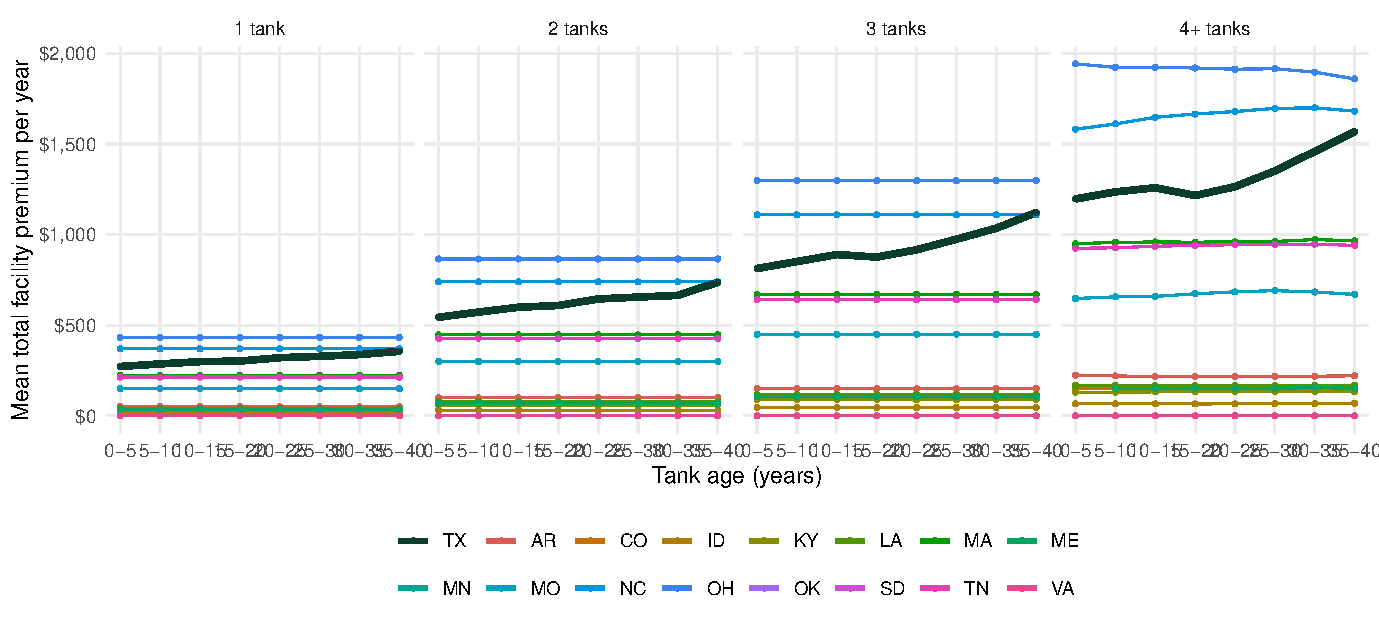
\includegraphics[width=0.97\textwidth,height=0.72\textheight,keepaspectratio]{../../Output/Figures/AE09_Premium_by_Age_State.pdf}
\end{center}

\vspace{0.05cm}

\centering\small\textit{Mean total facility premium by representative age band, one line per state, faceted by size (count held fixed, walls pooled). Texas (risk-based, bold) rises with age; every flat-fee state is flat in age ($P=\tau_s N$). The cross-state slope contrast at a given age and size is what pins $\gamma_{\text{price}}$.}
\end{frame}

\begin{frame}{Deductible \(\times\) hazard: the variation that
identifies \(\gamma_{\text{risk}}\)}
\phantomsection\label{deductible-times-hazard-the-variation-that-identifies-gamma_textrisk}
\BerkeleyLightMode

\vspace{0.1cm}
\begin{center}
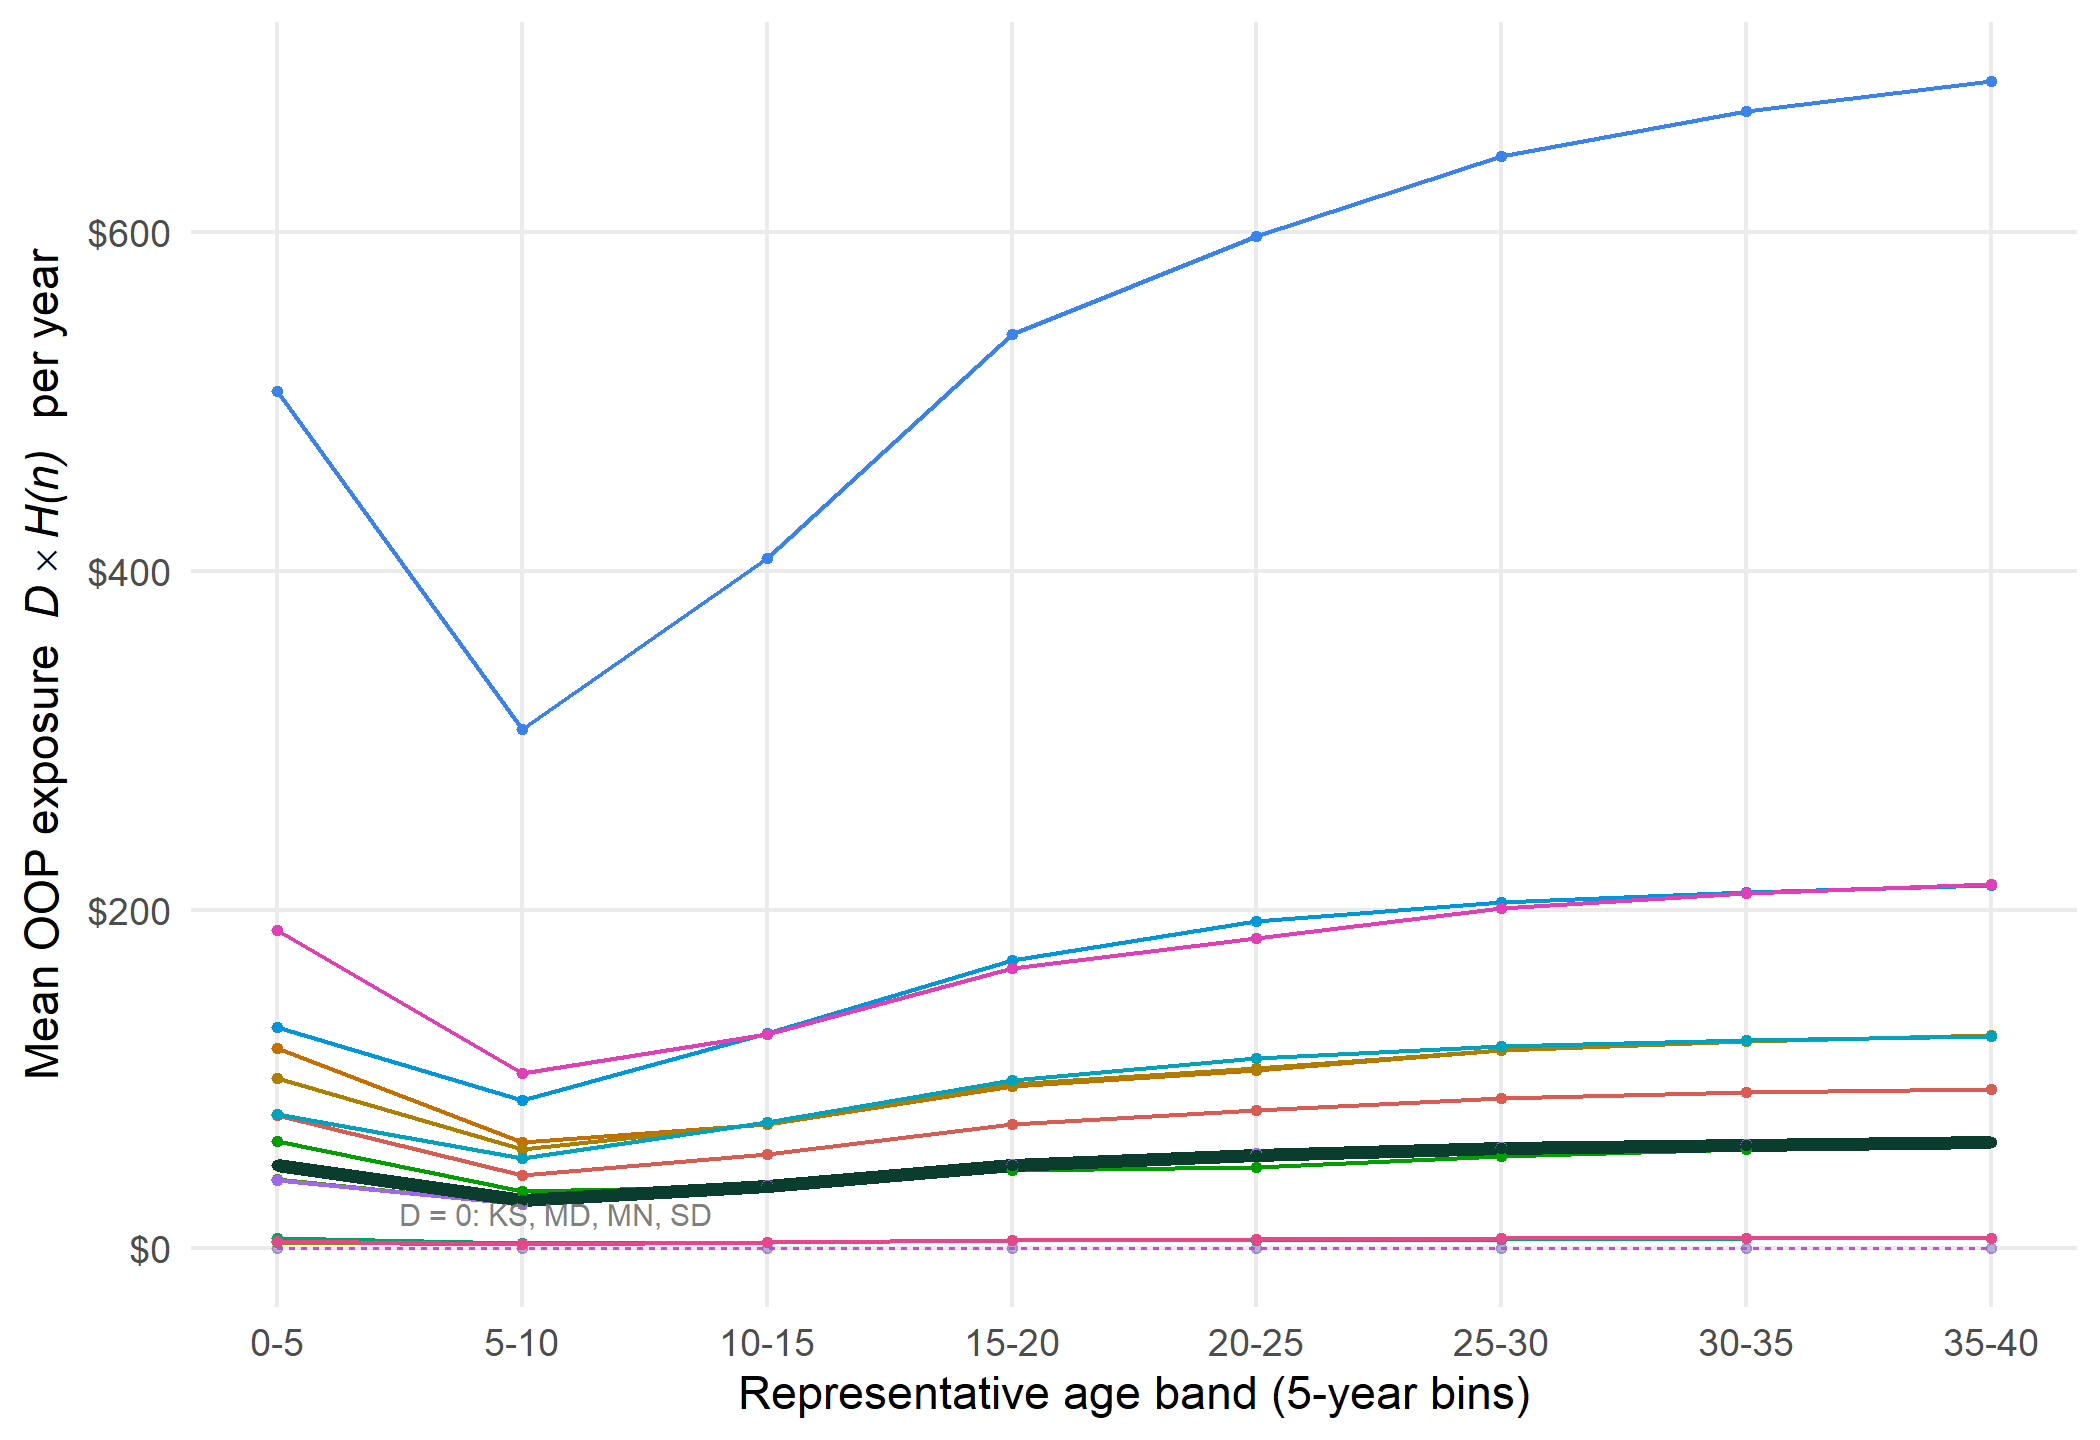
\includegraphics[width=0.92\textwidth,height=0.74\textheight,keepaspectratio]{../../Output/Figures/AE09_OOP_by_Age_Pooled.png}
\end{center}

\vspace{0.05cm}

\centering\small\textit{One point per state: deductible $D_s$ (vertical) against mean facility hazard (horizontal); whiskers span the within-state 10--90\% hazard range. Since $\mathrm{OOP}=\gamma_{\text{risk}}\,H(n)\,D_s$, the across-state deductible spread $\times$ the within-state hazard spread identifies $\gamma_{\text{risk}}$. Zero-deductible states (MN, SD, OK, VA) sit on the floor and contribute nothing.}
\end{frame}

\begin{frame}
\end{frame}

\end{document}
